\documentclass{configurations/polimi3i_thesis}

%------------------------------------------------------------------------------
%	REQUIRED PACKAGES AND  CONFIGURATIONS
%------------------------------------------------------------------------------

% CONFIGURATIONS
\usepackage{parskip} % For paragraph layout
\usepackage{setspace} % For using single or double spacing
\usepackage{emptypage} % To insert empty pages
\usepackage{multicol} % To write in multiple columns (executive summary)
\setlength\columnsep{15pt} % Column separation in executive summary
\setlength\parindent{0pt} % Indentation
\raggedbottom

% PACKAGES FOR TITLES
\usepackage{titlesec}
% \titlespacing{\section}{left spacing}{before spacing}{after spacing}
\titlespacing{\section}{0pt}{2.4ex}{1.4ex}
\titlespacing{\subsection}{0pt}{2.2ex}{1.1ex}
\titlespacing{\subsubsection}{0pt}{2.2ex}{0.8ex}
\usepackage{color}

% PACKAGES FOR LANGUAGE AND FONT
\usepackage[english]{babel} % The document is in English
\usepackage[utf8]{inputenc} % UTF8 encoding
\usepackage{lmodern} % Scalable fonts incl. bold typewriter at all sizes (fixes T1/cmtt/bx size warnings)
\usepackage[T1]{fontenc} % Font encoding
\usepackage[11pt]{moresize} % Big fonts

% PACKAGES FOR IMAGES
\usepackage{graphicx}
\usepackage{transparent} % Enables transparent images
\usepackage{eso-pic} % For the background picture on the title page
\usepackage{subfig} % Numbered and caption subfigures using \subfloat.
\usepackage{tikz} % A package for high-quality hand-made figures.
\usetikzlibrary{}
\graphicspath{{./images/}} % Directory of the images
\usepackage{caption} % Coloured captions
\usepackage{xcolor} % Coloured captions
\usepackage{amsthm,thmtools,xcolor} % Coloured "Theorem"
\usepackage{float}

% STANDARD MATH PACKAGES
\usepackage{amsmath}
\usepackage{amsthm}
\usepackage{amssymb}
\usepackage{amsfonts}
\usepackage{bm}
\usepackage[overload]{empheq} % For braced-style systems of equations.
\usepackage{fix-cm} % To override original LaTeX restrictions on sizes

% PACKAGES FOR TABLES
\usepackage{tabularx}
\usepackage{longtable} % Tables that can span several pages
\usepackage{xltabular} % longtable + tabularx X columns (page-breakable, width-distributing)
\usepackage{colortbl}

% PACKAGES FOR ALGORITHMS (PSEUDO-CODE)
\usepackage{algorithm}
\usepackage{algorithmic}

% PACKAGES FOR REFERENCES & BIBLIOGRAPHY
\usepackage[colorlinks=true,linkcolor=black,anchorcolor=black,citecolor=black,filecolor=black,menucolor=black,runcolor=black,urlcolor=black]{hyperref} % Adds clickable links at references
\usepackage{cleveref}
\usepackage[square, numbers, sort&compress]{natbib} % Square brackets, citing references with numbers, citations sorted by appearance in the text and compressed
\bibliographystyle{abbrvnat} % You may use a different style adapted to your field

% OTHER PACKAGES
\usepackage{pdfpages} % To include a pdf file
\usepackage{afterpage}
\usepackage{lipsum} % DUMMY PACKAGE
\usepackage{fancyhdr} % For the headers
\fancyhf{}

% Input of configuration file. Do not change config.tex file unless you really know what you are doing.
% Define blue color typical of polimi
\definecolor{bluepoli}{cmyk}{0.4,0.1,0,0.4}

% Custom theorem environments
\declaretheoremstyle[
  headfont=\color{bluepoli}\normalfont\bfseries,
  bodyfont=\color{black}\normalfont\itshape,
]{colored}

% Set-up caption colors
\captionsetup[figure]{labelfont={color=bluepoli}} % Set colour of the captions
\captionsetup[table]{labelfont={color=bluepoli}} % Set colour of the captions
\captionsetup[algorithm]{labelfont={color=bluepoli}} % Set colour of the captions

\theoremstyle{colored}
\newtheorem{theorem}{Theorem}[chapter]
\newtheorem{proposition}{Proposition}[chapter]

% Enhances the features of the standard "table" and "tabular" environments.
\newcommand\T{\rule{0pt}{2.6ex}}
\newcommand\B{\rule[-1.2ex]{0pt}{0pt}}

% Pseudo-code algorithm descriptions.
\newcounter{algsubstate}
\renewcommand{\thealgsubstate}{\alph{algsubstate}}
\newenvironment{algsubstates}
  {\setcounter{algsubstate}{0}%
   \renewcommand{\STATE}{%
     \stepcounter{algsubstate}%
     \Statex {\small\thealgsubstate:}\space}}
  {}

% New font size
\newcommand\numfontsize{\@setfontsize\Huge{200}{60}}

% Title format: chapter
\titleformat{\chapter}[hang]{
\fontsize{50}{20}\selectfont\bfseries\filright}{\textcolor{bluepoli} \thechapter\hsp\hspace{2mm}\textcolor{bluepoli}{|   }\hsp}{0pt}{\huge\bfseries \textcolor{bluepoli}
}

% Title format: section
\titleformat{\section}
{\color{bluepoli}\normalfont\Large\bfseries}
{\color{bluepoli}\thesection.}{1em}{}

% Title format: subsection
\titleformat{\subsection}
{\color{bluepoli}\normalfont\large\bfseries}
{\color{bluepoli}\thesubsection.}{1em}{}

% Title format: subsubsection
\titleformat{\subsubsection}
{\color{bluepoli}\normalfont\large\bfseries}
{\color{bluepoli}\thesubsubsection.}{1em}{}

% Shortening for setting no horizontal-spacing
\newcommand{\hsp}{\hspace{0pt}}

\makeatletter
% Renewcommand: cleardoublepage including the background pic
\renewcommand*\cleardoublepage{%
  \clearpage\if@twoside\ifodd\c@page\else
  \null
  \AddToShipoutPicture*{\BackgroundPic}
  \thispagestyle{empty}%
  \newpage
  \if@twocolumn\hbox{}\newpage\fi\fi\fi}
\makeatother

%For correctly numbering algorithms
\numberwithin{algorithm}{chapter}

%----------------------------------------------------------------------------
%	ADD YOUR DEFINITIONS AND COMMANDS (be careful of existing commands)
%----------------------------------------------------------------------------

% Let long monospaced identifiers wrap: allow a line break after every escaped
% underscore (snake_case) and absorb the few remaining tight lines, keeping
% \texttt{} paths and identifiers inside the text margins without hyphenation.
\renewcommand{\_}{\textunderscore\allowbreak}
\setlength{\emergencystretch}{3em}

% Placeholder figure box. Renders a labelled grey frame so the document compiles
% before the diagram exports exist. Usage:
%   \placeholderfig{5cm}{Caption of the diagram to be dropped in later}
% Replace the whole \placeholderfig{...}{...} call with an \includegraphics
% pointing at images/diagrams/<name> once the exported render is committed.
\newcommand{\placeholderfig}[2]{%
  \setlength{\fboxsep}{0pt}%
  \fcolorbox{gray!60}{gray!12}{%
    \parbox[c][#1][c]{0.86\linewidth}{%
      \centering
      \textbf{[\,FIGURE PLACEHOLDER\,]}\\[4pt]%
      \small\itshape #2%
    }%
  }%
}

% Digital-submission layout: open chapters on any page and turn \cleardoublepage
% into a plain \clearpage, so the PDF has no near-empty blank verso pages before
% chapters, the table of contents, or the end-matter lists.
\makeatletter
\@openrightfalse
\makeatother
\let\cleardoublepage\clearpage

%----------------------------------------------------------------------------
%	BEGIN OF YOUR DOCUMENT
%----------------------------------------------------------------------------

\begin{document}

\fancypagestyle{plain}{%
\fancyhf{} % Clear all header and footer fields
\fancyhead[RO,RE]{\thepage} %RO=right odd, RE=right even
\renewcommand{\headrulewidth}{0pt}
\renewcommand{\footrulewidth}{0pt}}

%----------------------------------------------------------------------------
%	TITLE PAGE
%----------------------------------------------------------------------------

\pagestyle{empty} % No page numbers
\frontmatter % Use roman page numbering style (i, ii, iii, iv...) for the preamble pages

\puttitle{
	title=Campus Arena\\DIMA Design Document, % Title of the thesis
	name1=Pica Mirko, % Author Name and Surname
    name2=Prendin Christian,
    name3=Saeed Abdullah,
	academicyear={2025-26},  % Academic Year
    releasedate=14/07/2026,
    version=1.0,
} % These info will be put into your Title page

\startpreamble
\setcounter{page}{1} % Set page counter to 1

%----------------------------------------------------------------------------
%	LIST OF CONTENTS/FIGURES/TABLES/SYMBOLS
%----------------------------------------------------------------------------

% TABLE OF CONTENTS
\thispagestyle{empty}
\tableofcontents % Table of contents
\thispagestyle{empty}
\cleardoublepage

\addtocontents{toc}{\vspace{2em}} % Add a gap in the Contents, for aesthetics
\mainmatter % Begin numeric (1,2,3...) page numbering

% ============================================================
%   CHAPTER 1 — INTRODUCTION
% ============================================================

\chapter{Introduction}
\label{ch:introduction}

\section{Project Purpose}
\label{sec:project_purpose}

\textit{CampusArena} was conceived from a concrete observation: the sports tables and courts scattered across the Politecnico di Milano campus host informal, untracked competitions with no record of outcomes, rankings, or achievements. The project began as \textit{PoliPONG}, a narrow utility for logging ping-pong results at a single table, and grew into a multi-sport competitive platform inspired by online rating ladders such as Chess.com but bound to \textbf{physical} play. Its core is a per-sport \textbf{ELO rating system} anchored to physical facilities, backed by a ``Proof of Play'' check-in mechanism: every ranked result is tied to a real location through a QR scan and to a confirming opponent through an in-app confirmation step.

That generalisation — from one PoliPONG table to any campus facility — drove the central architectural decision behind the system: the shared infrastructure (authentication, leaderboards, facility mapping, the match and queue flow) is sport-agnostic, while each sport's own rules and scoring sit behind a single shared contract, so a new discipline plugs in without touching the Core (\cref{sec:design_patterns}). \textbf{Ping Pong} and \textbf{Table Football} are the two disciplines delivered in this release; \textbf{Padel} and \textbf{3v3 Basketball} are documented extensions that the same contract and data model already accommodate (\cref{sec:project_scope}).

The application is deliberately not a social network: there are no posts, feeds, or public comment boards, and every interaction is anchored to a physical location and a competitive event. Keeping the surface this narrow is what keeps the system focused and hard to game — a broader social layer was never part of the product this was meant to be.

The remainder of this document proceeds from this purpose to the concrete feature set (\cref{ch:requirements_features}), the architecture and data model that realise it (\cref{ch:app_architecture}), the implementation choices behind the running app (\cref{ch:implementation_details}), its interface (\cref{ch:user_interface}), and the verification strategy that backs it (\cref{ch:testing_quality}).

% --------------------------------------------------------
\section{Project Scope}
\label{sec:project_scope}

The initial release of \textit{CampusArena} targets the Politecnico di Milano campus. The inventory of registered facilities — tables and courts, with their coordinates and QR identifiers — is provisioned by the team through a one-off seeding step; there is no in-app administration interface, since building one would add cost with no benefit for a fixed, small set of campus facilities.

\textbf{Sports in scope for the current delivery:}
\begin{itemize}
    \item \textbf{Ping Pong} — 1v1 singles and 2v2 doubles; set-based scoring. Facilities may be indoor or outdoor.
    \item \textbf{Table Football (Foosball)} — 1v1 singles and 2v2 doubles; goal-count scoring. Facilities may be indoor or outdoor.
\end{itemize}
\textbf{Padel} and \textbf{3v3 Basketball} are documented future extensions, not implemented in the current release: the \texttt{sportId} enumeration and the squad-size-agnostic data model already accommodate both, but neither has a scoring strategy, a result-entry screen, or a facility inventory.

\textbf{Delivered in this release:} dual-axis ELO ratings and leaderboards (global, per-sport, degree-program, and friends-filtered); a real-time, colour-coded facility map; QR-based Proof of Play check-in with a soft GPS presence audit; a digital per-facility queue; single-elimination tournaments with automatic seeding and byes; player and pair profiles with rating-trend statistics and achievements; friend-only direct challenges; the \textit{Arena Assistant}, a read-only in-app chatbot answering questions from live app data; and full English/Italian localisation across phone and tablet, light and dark themes.

\textbf{Out of scope} for the current release: court reservation/booking, real-money prize systems, multi-university support, in-app scheduling for direct challenges, an administration or moderation layer, and any form of user-generated content.

% --------------------------------------------------------
\section{Technology Stack}
\label{sec:technology_stack}

The technology choices are driven by three constraints: cross-platform delivery from a single codebase, real-time data synchronisation, and genuine integration of device hardware (camera, GPS) and external services beyond basic cloud storage. The entire stack runs within Firebase's free \textbf{Spark} tier; the consequences of that choice are made explicit in \cref{sec:trust_boundary}.

\begingroup
\small
\begin{xltabular}{\textwidth}{l l X}
    \caption{CampusArena technology stack.}\label{tab:tech_stack}\\
        \textbf{Layer} & \textbf{Technology} & \textbf{Rationale} \\\hline\\[-9px]
        \endfirsthead
        \multicolumn{3}{l}{\small\itshape \tablename~\thetable\ (continued)}\\[2px]
        \textbf{Layer} & \textbf{Technology} & \textbf{Rationale} \\\hline\\[-9px]
        \endhead
        UI Framework        & Flutter (Dart)               & Single codebase for Android \& iOS; \texttt{LayoutBuilder} / \texttt{MediaQuery} enable adaptive phone/tablet layouts. \\[3px]
        Authentication      & Firebase Auth                & Email/password registration and login; secure session/token management. \\[3px]
        Cloud Database      & Cloud Firestore              & Real-time snapshot streams for facility status, queues, and live ELO updates; atomic transactions; built-in offline persistence. \\[3px]
        Push Notifications  & Firebase Cloud Messaging     & Android only (no APNs on a free Apple Developer account). On the Spark tier there is no server sender, so queue/challenge alerts are client-local (\cref{sec:trust_boundary}). \\[3px]
        Map \& Tiles        & \texttt{flutter\_map} + OpenStreetMap & Interactive campus map with colour-coded availability pins. Keyless and billing-free; \texttt{flutter\_map\_cache} provides an on-disk tile cache honouring the OSM tile-usage policy. \\[3px]
        QR Scanner          & \texttt{mobile\_scanner}     & Hardware camera integration for Proof-of-Play check-in. \\[3px]
        GPS                 & \texttt{geolocator}          & Soft, non-blocking on-site presence audit at match initiation. \\[3px]
        Weather API         & Open-Meteo (REST)            & Keyless current conditions and forecasts for outdoor-facility evaluation. \\[3px]
        Arena Assistant     & LLM API (Regolo default)     & Natural-language Q\&A over a read-only tool layer via a deterministic intent-classified, grounded single LLM call; key injected via \texttt{-{}-dart-define}; rule-based fallback when unavailable. \\[3px]
        State Management    & \texttt{flutter\_bloc} (Cubit) & Unidirectional, testable state for auth, match sessions, queue, and every feature. \\[3px]
        Dependency Provision& \texttt{RepositoryProvider}  & Manual constructor injection; repositories provided to the tree and Cubits without a separate DI dependency. \\[3px]
        Routing             & \texttt{go\_router}          & Declarative deep linking; QR payload and notification routing; \texttt{StatefulShellRoute} tabs. \\[3px]
        Charts              & \texttt{fl\_chart}           & ELO trend graphs and statistics visualisations. \\[3px]
        Local Preferences   & \texttt{shared\_preferences} & Persists the Arena Assistant provider/model/key selection. \\[3px]
        Localisation        & \texttt{flutter\_localizations}, \texttt{intl} & English/Italian internationalisation via ARB resource files. \\[3px]
\end{xltabular}
\endgroup

% --------------------------------------------------------
\section{Definitions and Acronyms}
\label{sec:definitions_acronyms}

\begin{table}[H]
    \centering
    \small
    \begin{tabularx}{\textwidth}{l X}
        \textbf{Term} & \textbf{Meaning} \\\hline\\[-9px]
        ELO & Numerical skill rating; expected-score formula with K-factor weighting (\cref{sec:elo_algorithm}). \\[2px]
        K-factor & Multiplier controlling how strongly a single result moves a rating. \\[2px]
        Provisional phase & The first 10 rated matches for a given rating, played at a higher K-factor for faster convergence. \\[2px]
        Proof of Play & Integrity mechanism: QR check-in, soft GPS audit, and opponent confirmation. \\[2px]
        King of the Table & The player with the most confirmed wins at a given facility, denormalised on the facility document. \\[2px]
        Facility & A physical, registered table or court with a fixed location and QR code. \\[2px]
        Pair & A doubles team treated as its own rated entity via a deterministic \texttt{pairId}. \\[2px]
        Cubit & A lightweight, event-less unit of the \texttt{flutter\_bloc} state-management library. \\[2px]
        Isolate & A Dart execution unit with its own memory and event loop; true parallelism. \\[2px]
        FCM & Firebase Cloud Messaging (Android only in this project). \\[2px]
        ARB & Application Resource Bundle — Flutter's localisation file format. \\[2px]
        Spark tier & Firebase's free pricing tier; it excludes Cloud Functions. \\[2px]
        LLM & Large Language Model, used by the Arena Assistant. \\[2px]
        DIMA & Design and Implementation of Mobile Applications, the course this project was built for. \\[2px]
    \end{tabularx}
    \caption{Definitions, acronyms, and abbreviations used throughout this document.}
    \label{tab:definitions}
\end{table}

% ============================================================
%   CHAPTER 2 — REQUIREMENTS AND FEATURES
% ============================================================

\chapter{Requirements and Features}
\label{ch:requirements_features}

\section{Functional Requirements}
\label{sec:functional_requirements}

The functional scope is divided between the sport-agnostic Core services and the sport-specific scoring logic. This separation is enforced structurally through a shared scoring contract, ensuring that each part is independently testable and that new sports can be added with localised changes.

\subsection{Core System Requirements}

\begin{itemize}
    \item \textbf{Authentication:} register and authenticate users via Firebase Auth (email/password), managing sessions and secure tokens. A unique, case-insensitive username is claimed atomically at registration.
    \item \textbf{Global Leaderboard Aggregator:} maintain a synchronised campus-wide ranking updated in real time after every confirmed result. Filters: global, per-sport, friends-only, and \textbf{Course Rivalry} (by degree program).
    \item \textbf{Competitive Profile:} a profile strictly limited to performance analytics — per-sport ELO and match counts, win/loss and streaks, an interactive rating-trend graph, badge achievements, and facility metrics. No social feeds, timelines, or comment boards.
    \item \textbf{Geographic Facility Mapping:} render an interactive campus map via \texttt{flutter\_map}\slash\allowbreak OpenStreetMap with real-time, colour-coded availability markers: \emph{Free} (green), \emph{Occupied} (red, with elapsed timer and active players), or \emph{Queued} (yellow).
    \item \textbf{Weather Data Integration:} for each \emph{outdoor} facility, asynchronously retrieve current conditions from Open-Meteo (temperature, precipitation, wind) and surface them in the facility detail card; for tournaments on outdoor facilities, surface a short-term forecast for the scheduled timeslot. The \texttt{isOutdoor} flag is the single source of truth for weather visibility; indoor facilities display no weather.
    \item \textbf{Notification Dispatch:} the Spark tier has no server-side push sender, so alerts are \emph{client-local} — a player's own listener detects the event and raises an in-app banner/SnackBar with haptic feedback (\cref{sec:trust_boundary}). Two classes are dispatched this way: reaching the front of a facility queue, and receiving a Direct Challenge. Tournament bracket progress carries no separate alert; it is surfaced passively through the bracket screen's own live listener.
    \item \textbf{Offline Persistence:} rely on Firestore's built-in offline persistence to keep leaderboards, profiles, and histories viewable when the network is unavailable.
    \item \textbf{Arena Assistant:} a read-only, in-app natural-language assistant answering questions about live app data and static app knowledge (\cref{sec:assistant_arch}).
\end{itemize}

\subsection{Sport-Specific Requirements}

\begin{itemize}
    \item \textbf{Contextual Matchmaking:} each module manages localised physical matchmaking, digital queue processing, and friends-only Direct Challenges for its discipline.
    \item \textbf{Proof of Play \& Hardware Verification:} to initiate a ranked match, the module activates the native camera to scan the QR code on the physical table (with a printed alphanumeric fallback code). The GPS service records the distance from the facility as a \textbf{soft, non-blocking} audit signal; check-in is \textbf{never blocked} on GPS, since indoor and covered facilities exhibit significant drift. Integrity rests on physical QR presence plus dual opponent confirmation.
    \item \textbf{Isolated Scoring Contracts:} each module implements the shared \texttt{ScoringStrategy} interface, encoding sport-specific rules and maintaining an isolated ELO rating per player/team.
    \item \textbf{Dual Result Confirmation:} submission requires explicit in-app confirmation from the opponent; ELO recalculation executes only after that confirmation. A rejected result is marked \texttt{Disputed} with no ELO change and both players notified; a result left unconfirmed, or a match abandoned before any result is submitted, times out with no ELO change and frees the facility. Repeated abuse of disputes ($\geq 3$) triggers a 7-day cooldown during which the offender's dispute attempts are intercepted.
    \item \textbf{Tournament Lifecycle:} support single-elimination tournament creation with automatic seeding and byes for non-power-of-two counts; the organiser advances slots and records forfeits. If registration does not fill, the tournament proceeds at the deadline with a smaller, re-seeded bracket. Live standings are maintained and a tournament ELO multiplier is applied.
    \item \textbf{Achievements:} six client-side badges (\cref{sec:data_model}) are evaluated inside the match-confirmation transaction.
\end{itemize}

% --------------------------------------------------------
\section{Non-Functional Requirements}
\label{sec:non_functional_requirements}

\begin{itemize}
    \item \textbf{Extensibility:} a new sport must require only a new \texttt{ScoringStrategy} implementation and its result-entry UI, with no modifications to the Core services.
    \item \textbf{Reliability \& Data Consistency:} match-result and queue-position writes must be atomic (Firestore transactions), so ELO updates and queue ordering can never be left in a partial or inconsistent state, even under concurrent access.
    \item \textbf{Data Integrity via Proof of Play:} a ranked result is recorded only after a QR-based check-in and explicit dual confirmation. GPS is a soft audit signal and never gates check-in.
    \item \textbf{Portability \& Look-and-Feel:} a single Material~3 design language and a fully internationalised (EN/IT) UI across Android and iOS, responsive from phone to tablet.
\end{itemize}

% --------------------------------------------------------
\section{Constraints}
\label{sec:constraints}

\begin{itemize}
    \item \textbf{Free backend tier.} The Spark tier excludes Cloud Functions, so there is no server-side code. Timeouts are evaluated lazily by clients, achievements are evaluated client-side inside the confirmation transaction, and queue-ready alerts are client-local.
    \item \textbf{iOS push disabled.} APNs requires a paid Apple Developer account, so FCM is configured for Android only; the rest of the iOS build works normally and \texttt{PushTokenService} degrades to a no-op where messaging is unavailable.
    \item \textbf{Connectivity for ranked play.} Firestore's offline persistence keeps leaderboards, profiles, and recent data readable offline, but ranked play requires connectivity by design: QR check-in and live opponent confirmation are the integrity mechanism, and an offline write-and-sync path for ELO would create a distributed-consistency problem that undermines it (\cref{sec:data_model}).
    \item \textbf{Multi-device support.} The same codebase serves phones and tablets; the layout adapts at a 600\,dp breakpoint (\cref{sec:responsive}).
\end{itemize}

% --------------------------------------------------------
\section{Actors}
\label{sec:actors}

\begin{table}[H]
    \centering
    \small
    \begin{tabularx}{\textwidth}{l X}
        \textbf{Actor} & \textbf{Description} \\\hline\\[-9px]
        \textbf{Player} & Any registered user. Checks in at facilities, plays ranked singles or doubles matches, joins queues, climbs leaderboards, adds friends, sends challenges, earns achievements, and queries the Arena Assistant. \\[3px]
        \textbf{Tournament Organiser} & A Player who creates a tournament and thereby gains organiser controls over that bracket: seeding at the deadline, advancing slots, and marking forfeits. Per-tournament, not a separate account type. \\[3px]
        \textbf{Opponent} & The counterpart Player in a match. Their confirmation is what makes a result count — a structural role within the match flow, not a distinct account. \\[3px]
        \textbf{External systems} & Firestore real-time listeners, FCM, Open-Meteo, the OpenStreetMap tile servers, and the Regolo LLM endpoint. Collaborators of the client, not human actors. \\[3px]
    \end{tabularx}
    \caption{Actors.}
    \label{tab:actors}
\end{table}

% --------------------------------------------------------
\section{Use Cases}
\label{sec:use_case_diagrams}

Result submission and confirmation are included in every ranked match; every tournament round is played through the same ranked match flow.

\begin{itemize}
    \item \textbf{UC\_1:} Register / Authenticate and Load Profile
    \item \textbf{UC\_2:} Browse Live Facility Map
    \item \textbf{UC\_3:} Execute Match via Proof-of-Play Check-In
    \item \textbf{UC\_4:} Complete Game and Recalculate ELO
    \item \textbf{UC\_5:} Join Facility Queue \& Receive Alert
    \item \textbf{UC\_6:} Create and Participate in a Tournament
    \item \textbf{UC\_7:} Send / Accept a Friend Challenge
    \item \textbf{UC\_8:} Ask the Arena Assistant about live app state
\end{itemize}

\begin{figure}[H]
    \centering
    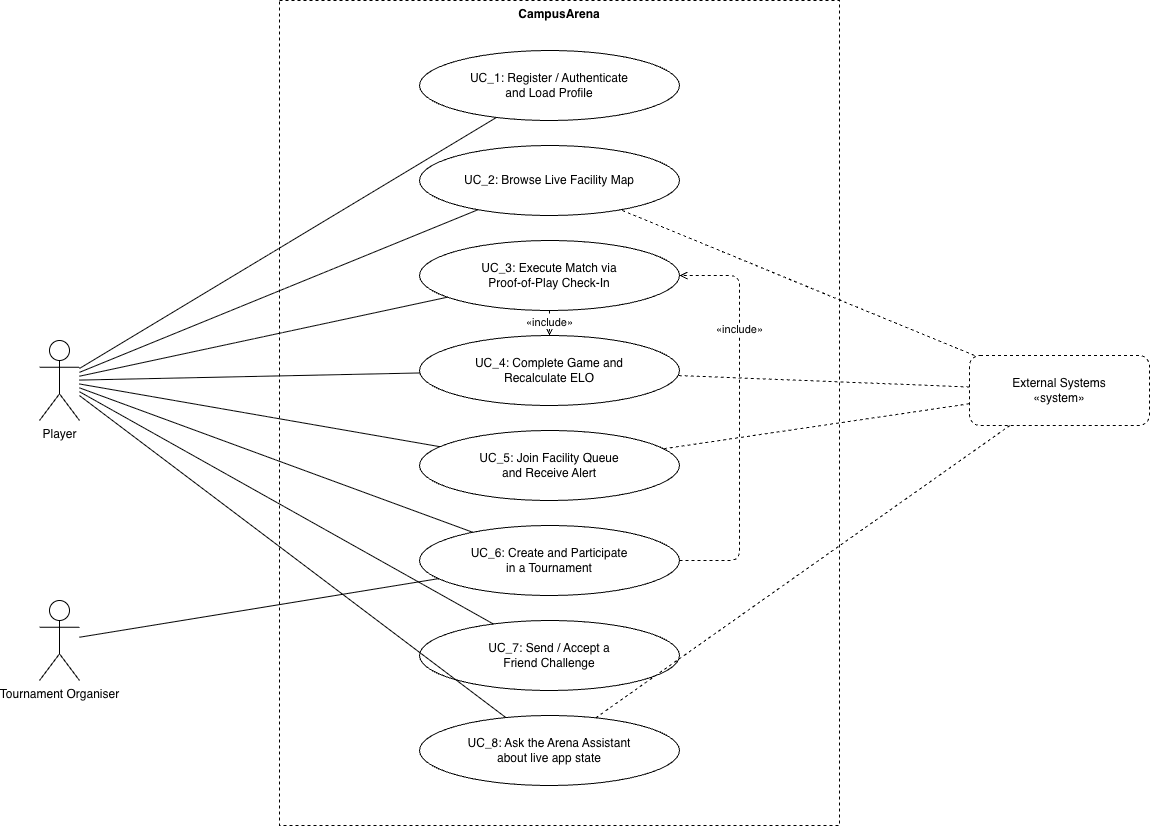
\includegraphics[width=0.9\textwidth]{diagrams/usecase}
    \caption{CampusArena use-case diagram.}
    \label{fig:usecase}
\end{figure}

\textbf{Ranked match (core loop).} A player taps Play, scans the QR sticker on a free table (or types the printed fallback code). The app logs the GPS distance as a soft audit value, creates a match document, and flips the facility to \emph{occupied} on every user's map in real time. The opponent joins by scanning the same code. When the game ends, one player enters the score through a sport-specific entry form; the other confirms or disputes it on their own device. On confirmation, a single Firestore transaction applies the ELO exchange, updates both ratings, frees the facility, refreshes the King of the Table, and awards any newly earned achievements.

\textbf{Tournament.} Any player creates a single-elimination tournament for a sport at a facility, with a participant cap and a registration deadline. Players register; at the deadline the bracket is seeded, assigning byes automatically when the count is not a power of two. Each bracket slot is played as a normal ranked match carrying the tournament context, and the confirmed result advances the winner. The organiser can mark no-shows as forfeits. Winning the final applies a $1.5\times$ ELO multiplier and the Tournament Champion badge.

% --------------------------------------------------------
\section{Screen Inventory}
\label{sec:screen_inventory}

The delivered app contains \textbf{29 distinct screens}, routed with \texttt{go\_router} and \texttt{StatefulShellRoute}. The match and result flows are staged inside two container pages (\texttt{MatchFlowPage}, \texttt{ResultFlowPage}) that orchestrate their stages as full-screen views driven by \texttt{MatchCubit}/\texttt{ResultCubit} state, so each stage below is a distinct screen the user experiences even where several share one route.

\begin{table}[H]
    \centering
    \small
    \begin{tabularx}{\textwidth}{r X l}
        \# & \textbf{Screen} & \textbf{Route} \\\hline\\[-9px]
        1--5   & Splash, Landing, Login, Register, Forgot Password & \texttt{/}, \texttt{/landing}, \ldots \\[2px]
        6      & Mini-Tutorial & \texttt{/onboarding/tutorial} \\[2px]
        7      & Home / Dashboard & \texttt{/home} \\[2px]
        8--10  & Map view, Facility list view, Facility detail & \texttt{/map} (+ overlay) \\[2px]
        11     & Leaderboards (global/sport/degree/friends, search) & \texttt{/leaderboards} \\[2px]
        12--14 & Own profile \& stats, Public player profile, Team (pair) profile & \texttt{/profile}, \texttt{/profile/:uid}, \texttt{/team/:pairId} \\[2px]
        15--17 & Friends, Settings, Privacy & \texttt{/friends}, \texttt{/settings} \\[2px]
        18--23 & QR scan, Match setup, Active match, Score entry, Result review, Match summary & \texttt{/play/\dots}, \texttt{/match/:id/result} \\[2px]
        24     & Challenge respond & \texttt{/challenge/:id} \\[2px]
        25--28 & Tournament browser, Create, Detail, Live bracket & \texttt{/tournaments}\ldots \\[2px]
        29     & Arena Assistant chat (+ its settings screen) & \texttt{/chatbot} \\[2px]
    \end{tabularx}
    \caption{Screen inventory grouped by functional area (29 screens). Renders appear in \cref{ch:user_interface}.}
    \label{tab:screen_inventory}
\end{table}

% --------------------------------------------------------
\section{Requirements Traceability}
\label{sec:traceability}

Each functional requirement traces to the state component, repository/domain logic, and data that implement it.

\begingroup
\small
\begin{xltabular}{\textwidth}{%
    >{\hsize=1.1\hsize\raggedright\arraybackslash}X%
    >{\hsize=.8\hsize\raggedright\arraybackslash}X%
    >{\hsize=1.1\hsize\raggedright\arraybackslash}X}
    \caption{Requirements traceability matrix.}\label{tab:traceability}\\
        \textbf{Requirement} & \textbf{State component} & \textbf{Repository / domain \& data} \\\hline\\[-9px]
        \endfirsthead
        \multicolumn{3}{l}{\small\itshape \tablename~\thetable\ (continued)}\\[2px]
        \textbf{Requirement} & \textbf{State component} & \textbf{Repository / domain \& data} \\\hline\\[-9px]
        \endhead
        Registration, login, unique usernames & \texttt{AuthCubit} & \texttt{AuthRepository}, \texttt{UserRepository} (username claim txn); \texttt{users}, \texttt{usernames} \\[3px]
        Per-sport ELO, provisional K, lazy decay & \texttt{ResultCubit}, \texttt{ProfileCubit} & \texttt{EloCalculator}, \texttt{RatingRepository}, \texttt{MatchRepository}; \texttt{ratings}, \texttt{matches} \\[3px]
        Doubles pair ratings & \texttt{ResultCubit}, \texttt{TeamProfileCubit} & \texttt{pairIdFromUids}, \texttt{getOrCreatePairRating}; \texttt{ratings} (pair) \\[3px]
        Facility map with live status & \texttt{FacilityCubit} & \texttt{FacilityRepository}, \texttt{buildOsmTileProvider}; \texttt{facilities}, OSM tiles \\[3px]
        Weather (outdoor facilities/tournaments) & \texttt{WeatherCubit} & \texttt{WeatherRepository}; Open-Meteo \\[3px]
        QR check-in, fallback code, GPS audit & \texttt{MatchCubit} & \texttt{MatchRepository}\allowbreak\texttt{.createMatch}, \texttt{mobile\_scanner}, \texttt{geolocator}; \texttt{matches}, \texttt{facilities} \\[3px]
        Queue with soft enforcement \& alert & \texttt{QueueCubit} & \texttt{QueueRepository}, facility stream; \texttt{facilities/\{id\}/queue} \\[3px]
        Result entry, confirmation, dispute & \texttt{ResultCubit} & \texttt{ScoringStrategy}+factory, \texttt{MatchRepository}\allowbreak\texttt{.confirm}\slash\allowbreak\texttt{disputeResult}; \texttt{matches}, \texttt{ratings}, \texttt{users} \\[3px]
        Lazy timeouts (abandoned/unconfirmed) & any reading client & \texttt{MatchRepository}\allowbreak\texttt{.resolveTimeout}; \texttt{matches}, \texttt{facilities} \\[3px]
        Leaderboards with filters and search & \texttt{LeaderboardCubit} & \texttt{RatingRepository}, \texttt{UserRepository}; \texttt{ratings} (composite indexes) \\[3px]
        Profile statistics \& ELO trend chart & \texttt{ProfileCubit} (isolate) & \texttt{MatchRepository}, \texttt{RatingRepository}, \texttt{fl\_chart}; \texttt{matches}, \texttt{ratings} \\[3px]
        Achievements (6 badges) & inside confirmation & \texttt{AchievementEvaluator}, \texttt{AchievementRepository}; \texttt{users.badges}, \texttt{achievementDefs} \\[3px]
        Friends and direct challenges & \texttt{FriendsCubit}, \texttt{ChallengeCubit} & \texttt{UserRepository}, \texttt{ChallengeRepository}; \texttt{users.friendUids}, \texttt{challenges} \\[3px]
        Single-elimination tournaments with byes & tournament Cubits & \texttt{TournamentRepository}, \texttt{bracket\_engine.dart}; \texttt{tournaments}, \texttt{participants}, \texttt{matches} \\[3px]
        Arena Assistant with fallback \& disclaimer & \texttt{ChatCubit}, \texttt{AssistantSettingsCubit} & \texttt{ChatbotRepository}, \texttt{ChatbotToolsService}, \texttt{LlmClient}, \texttt{RuleBasedIntentMatcher}; read-only over existing collections, Regolo API \\[3px]
        EN/IT localisation & \texttt{LocaleCubit} & ARB files, \texttt{intl}; \texttt{users.language} \\[3px]
        Phone and tablet layouts & \texttt{AppShell}, per screen & \texttt{LayoutBuilder} / \texttt{MediaQuery} \\[3px]
\end{xltabular}
\endgroup

% ============================================================
%   CHAPTER 3 — APPLICATION ARCHITECTURE
% ============================================================

\chapter{Application Architecture}
\label{ch:app_architecture}

\section{Overview and Layering}
\label{sec:high_level_overview}

CampusArena is a single Flutter client organised into four layers. Dependencies point strictly downward: no lower layer imports an upper one, and only the repository layer talks to Firebase or the network.

\begin{itemize}
    \item \textbf{Presentation} (\texttt{lib/features/*/\dots\_screen.dart}, \texttt{lib/routing/}) renders state and forwards user intent. It holds only ephemeral UI state (tab index, form fields, animation controllers) through state hoisting: data down, callbacks up.
    \item \textbf{Application State} (\texttt{lib/features/*/cubit/}) contains one Cubit per use case (21 in total). A Cubit calls repositories, runs domain logic, and emits immutable \texttt{Equatable} states consumed through \texttt{BlocBuilder}/\texttt{BlocListener}. The team chose Cubit over the full BLoC event layer: with a three-person team learning the library from zero, the event indirection added ceremony without adding testability, since \texttt{bloc\_test} exercises Cubit methods just as directly.
    \item \textbf{Core Domain} (\texttt{lib/core/}, \texttt{lib/models/}) is framework-free Dart: \texttt{EloCalculator}, the \texttt{ScoringStrategy} family with its factory, the bracket-derivation module (\texttt{bracket\_engine.dart}: \texttt{build}, \texttt{BracketTree}\slash\allowbreak\texttt{BracketSlot}\slash\allowbreak\texttt{BracketSide}), \texttt{AchievementEvaluator}, and the ten immutable model classes (\texttt{UserModel}, \texttt{RatingModel}, \texttt{FacilityModel}, \texttt{QueueEntryModel}, \texttt{MatchModel}, \texttt{TournamentModel}, \texttt{TournamentParticipantModel}, \texttt{ChallengeModel}, \texttt{AchievementDefModel}, \texttt{ChatMessageModel}). Nothing here imports Flutter or Firebase except localised \texttt{Timestamp} conversions in the model serializers, so the competitive rules are unit-testable in plain Dart.
    \item \textbf{Repositories} (\texttt{lib/repositories/}) form the only boundary to persistence and the network. Each of the ten repositories wraps one Firestore collection or one external API and exposes typed streams and futures. Tests substitute them with \texttt{mocktail} mocks or run them against \texttt{fake\_cloud\_firestore}.
\end{itemize}

\begin{figure}[H]
    \centering
    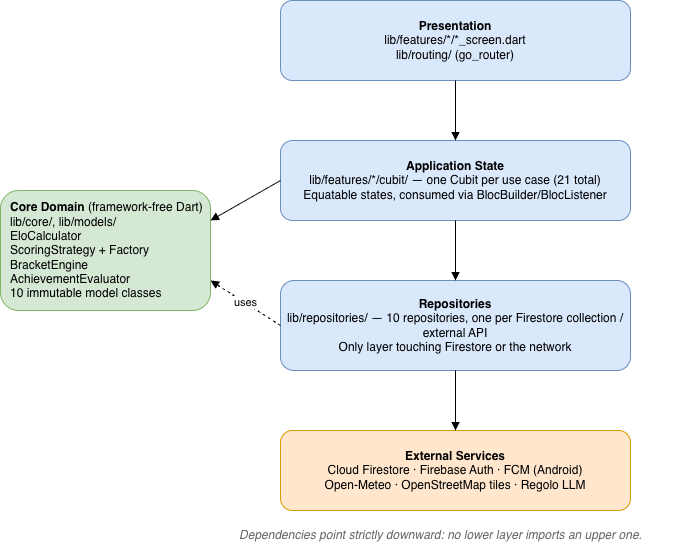
\includegraphics[width=0.9\textwidth]{diagrams/architecture}
    \caption{Layered architecture with strictly downward dependencies.}
    \label{fig:architecture}
\end{figure}

\section{Component View}
\label{sec:component_view}

\begin{table}[H]
    \centering
    \small
    \begin{tabularx}{\textwidth}{l X}
        \textbf{Component} & \textbf{Responsibility} \\\hline\\[-9px]
        \texttt{AuthRepository} & Firebase Auth: sign up/in/out, password reset, and the \texttt{authStateChanges} stream that drives the router guard. \\[3px]
        \texttt{UserRepository} & CRUD on \texttt{users/\{uid\}}; the registration transaction that claims \texttt{usernames/\{username\}} atomically with the profile; friend-list updates; player search by username prefix. \\[3px]
        \texttt{RatingRepository} & Owns \texttt{ratings} for users and pairs: seeding one rating per sport at registration, get-or-create for pair ratings, leaderboard queries, rank computation. \\[3px]
        \texttt{FacilityRepository} & Streams facilities and single-facility status; bounded one-shot status queries for the chatbot. \\[3px]
        \texttt{QueueRepository} & Transactional join/leave with a monotonic ticket counter; queue streams; \texttt{count()} aggregation for queue length. \\[3px]
        \texttt{MatchRepository} & The match lifecycle: create with lazy queue eviction, join, submit, confirm, dispute, and lazy timeout resolution. All state transitions run in Firestore transactions. \\[3px]
        \texttt{TournamentRepository} & Tournament CRUD, transactional registration with a denormalised participant counter, seeding at the deadline, bracket-map updates. \\[3px]
        \texttt{ChallengeRepository} & Friend-only challenge documents: send, accept, decline, expiry. \\[3px]
        \texttt{AchievementRepository} & Reads the seeded \texttt{achievementDefs} for badge rendering and evaluation input. \\[3px]
        \texttt{WeatherRepository} & Open-Meteo REST calls: current conditions and a bounded hourly forecast window. \\[3px]
        \texttt{ChatbotToolsService} & The read-only tool layer of the Arena Assistant: bounded one-shot queries over the existing repositories, never a write, never a listener. \\[3px]
        \texttt{ChatbotRepository} & Orchestrates the assistant: intent classification, tool execution, system-prompt assembly, the single LLM call, and the rule-based fallback. \\[3px]
        \texttt{bracket\_engine.dart} & Pure derivation of the bracket tree from participants, the persisted round map, and match documents: seed placement, byes, winner resolution, forfeit handling. \\[3px]
        \texttt{AchievementEvaluator} & Pure evaluation of the six badge conditions against the confirmed match, recent history, and facility data prepared before the transaction. \\[3px]
    \end{tabularx}
    \caption{Principal components and their responsibilities.}
    \label{tab:components}
\end{table}

\section{Design Patterns}
\label{sec:design_patterns}

\begin{itemize}
    \item \textbf{Repository pattern.} One repository per aggregate; the only layer touching Firestore or HTTP. This is what makes the test campaign possible: Cubit tests mock repositories with \texttt{mocktail}, and repository tests run against \texttt{fake\_cloud\_firestore}.
    \item \textbf{Unidirectional state (Cubit).} UI calls a Cubit method; the Cubit awaits repositories and emits a new immutable state; \texttt{BlocBuilder} rebuilds. No two-way binding anywhere.
    \item \textbf{Strategy.} \texttt{ScoringStrategy} abstracts per-sport rules behind \texttt{validateResult}, \texttt{getResultWidget}, and \texttt{computeMatchOutcome}. \texttt{PingPongScoringStrategy} validates set arrays (win by 2, at least 11 points, no tied sets, majority of sets); \texttt{FoosballScoringStrategy} validates a single game. Each strategy owns the serialisation shape of its result map, so adding padel means one new class and one factory branch, with no change to the match flow.
    \item \textbf{Factory.} \texttt{ScoringStrategyFactory.forSport(sportId)} resolves the strategy and throws \texttt{UnsupportedSportException} for sports that are modelled but not yet playable — exactly how padel is kept out of the UI while remaining in the schema.
    \item \textbf{Observer.} Firestore \texttt{snapshots()} streams drive the live surfaces (facility pins, queue position, active match, bracket) without polling. \texttt{GoRouterRefreshStream} adapts the \texttt{AuthCubit} stream to a \texttt{ChangeNotifier} so the router re-evaluates its redirect on every auth change.
    \item \textbf{Deterministic identifiers as idempotency keys.} \texttt{ratingId = \{sportId\}\_\{ownerId\}}, \texttt{pairId} = sorted UIDs joined with \texttt{\_}, queue ticket ID = the player's UID, username claim ID = the lowercased handle. Repeated writes resolve to the same document, making transactions safe to retry and enabling direct lookups without queries.
\end{itemize}

\section{Data Model}
\label{sec:data_model}

The backend store is \textbf{Cloud Firestore}, a document database without joins. The model denormalises frequently-read fields onto the documents that read them (\texttt{facility.status}, \texttt{rating.degreeProgram}, \texttt{tournament.participantCount}), keeps small always-read-together data as parent fields (\texttt{friendUids}, \texttt{badges}), and promotes independently-queried or per-entity-writable data to subcollections (\texttt{queue}, \texttt{participants}). Composite indexes for every multi-field query are declared in \texttt{app/firestore.indexes.json}.

\subsection{Collections}

\begin{table}[H]
    \centering
    \small
    \begin{tabularx}{\textwidth}{l l X}
        \textbf{Collection} & \textbf{Doc ID} & \textbf{Purpose} \\\hline\\[-9px]
        \texttt{users/\{uid\}} & Firebase Auth UID & Identity, friends, badges, language, onboarding gate, dispute counters. \\[3px]
        \texttt{usernames/\{username\}} & lowercased handle & Immutable uniqueness reservation, claimed atomically with the user doc. \\[3px]
        \texttt{ratings/\{ratingId\}} & \texttt{sportId\_ownerId} & Per-sport ELO for \emph{both} users and pairs (\texttt{ownerType}); the single leaderboard source. \\[3px]
        \texttt{facilities/\{facilityId\}} & auto-ID & Physical tables; denormalised live \texttt{status}, King of the Table, \texttt{isOutdoor}. \\[3px]
        \texttt{facilities/\{id\}/queue/\{uid\}} & UID & Per-facility queue entries (subcollection). \\[3px]
        \texttt{matches/\{matchId\}} & auto-ID & Ranked match documents and lifecycle state. \\[3px]
        \texttt{tournaments/\{tournamentId\}} & auto-ID & Single-elimination tournaments and bracket map. \\[3px]
        \texttt{tournaments/\{id\}/participants/\{uid\}} & UID & Per-participant seed / elimination (subcollection). \\[3px]
        \texttt{challenges/\{challengeId\}} & auto-ID & Friend-only direct challenges. \\[3px]
        \texttt{achievementDefs/\{id\}} & slug & Read-only badge definitions (seeded). \\[3px]
    \end{tabularx}
    \caption{Firestore collections.}
    \label{tab:collections}
\end{table}

\subsection{Key Schema Decisions}

\begin{itemize}
    \item \textbf{\texttt{ratings} is top-level, not embedded on users.} The global leaderboard becomes a single composite-indexed query — \texttt{ratings.where(sportId==X)}\allowbreak\texttt{.where(ownerType==user)}\allowbreak\texttt{.orderBy(elo desc)}\allowbreak\texttt{.limit(100)} — and the course-rivalry leaderboard adds one \texttt{where(degreeProgram==Y)}. Singles and doubles share one collection, one repository, one K-factor/decay function.
    \item \textbf{Doubles pairs are rated entities in \texttt{ratings}}, keyed by a deterministic \texttt{pairId} (sorted UIDs) with \texttt{ownerType=pair} — \emph{not} an average of singles ratings, and \emph{not} a separate collection. This yields an independent doubles leaderboard for free.
    \item \textbf{No cached counters on the user doc.} ELO and \texttt{matchesPlayed} live only in \texttt{ratings}; streaks are derived from match history at read time. Single source of truth, no desync.
    \item \textbf{\texttt{facility.status}/\texttt{currentMatchId} are denormalised}, written by the match flow, so the map's status listener never cross-reads \texttt{matches}.
    \item \textbf{Queue and participants are subcollections} (not array fields) so a position/seed listener does not re-fire on unrelated parent-doc changes and each entry is individually writable.
    \item \textbf{\texttt{queueTailPosition} is a monotonic ticket counter} recording the highest ticket ever issued; it is never decremented or renumbered on leave. Display rank is derived from the ordered snapshot index on the client.
    \item \textbf{The match document carries its own denormalised keys.} A doubles match stores \texttt{team1PairId}/\texttt{team2PairId} (rather than deriving them), so ``all matches for this pair'' is a direct query; and its \texttt{result} map's score shape is owned by the sport's \texttt{ScoringStrategy} (per-set points for ping pong, goal counts for foosball), keeping the match schema sport-agnostic.
\end{itemize}

\begin{figure}[H]
    \centering
    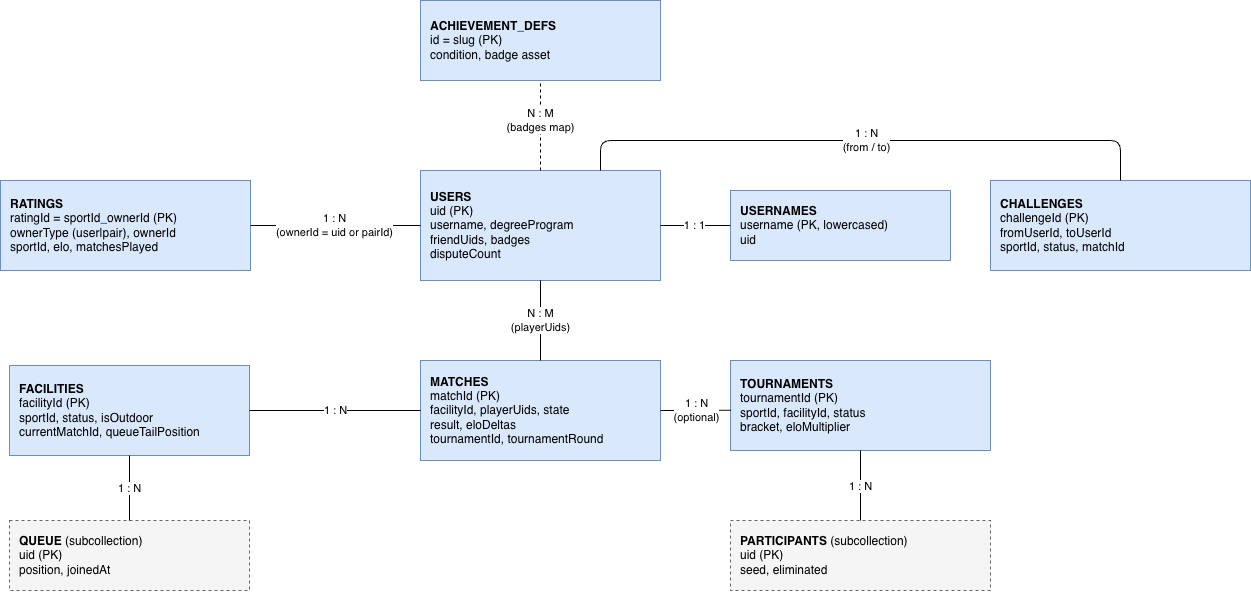
\includegraphics[width=0.9\textwidth]{diagrams/er}
    \caption{Firestore entity-relationship overview.}
    \label{fig:er}
\end{figure}

\subsection{Offline Persistence Strategy}
The system relies on Firestore's built-in offline persistence to cache reads, ensuring offline accessibility for leaderboards and profiles. Ranked match writes assert network connectivity to preserve Proof of Play. There is no local SQLite database and no offline match write-and-sync path; the only on-device stores are the OSM tile cache (a drift/SQLite store required by the tile-usage policy) and \texttt{shared\_preferences} for the assistant settings.

\section{Match State Machine}
\label{sec:match_state}

The match lifecycle is a small state machine whose timeout transitions run without any server: they are evaluated lazily by whichever client next reads the facility or scans its QR code, inside a transaction that also frees the facility.

\texttt{free} is not a match state; it is the absence of an active match, represented by \texttt{facility.status = free}. The concrete thresholds live in \texttt{MatchRepository}: \texttt{occupiedTimeout = 4\,hours} and \texttt{awaitingConfirmationTimeout = 24\,hours}, both measured from \texttt{startedAt} and applied by \texttt{resolveTimeout}. All terminal states except \texttt{confirmed} leave ratings untouched and free the facility.

\begin{figure}[H]
    \centering
    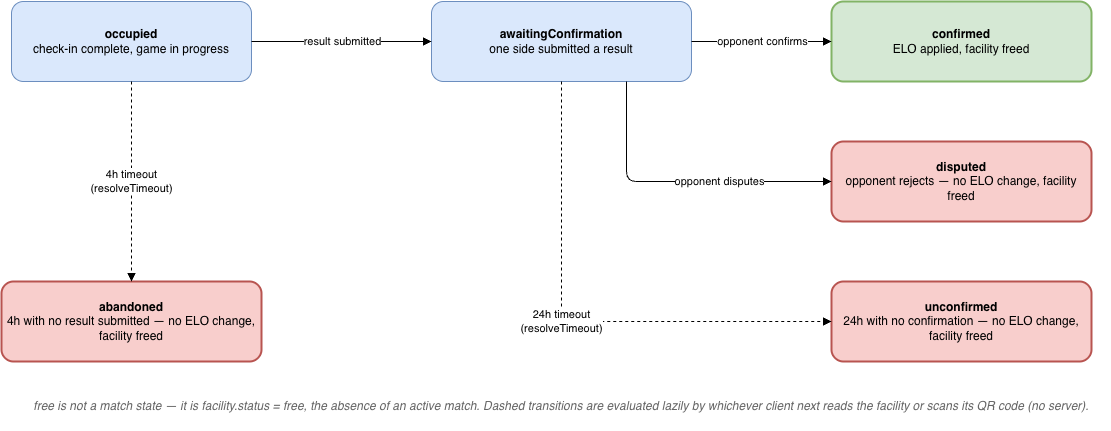
\includegraphics[width=0.9\textwidth]{diagrams/match_state}
    \caption{Ranked-match state machine with lazy timeout transitions.}
    \label{fig:match_state}
\end{figure}

\section{Trust Boundary and Security}
\label{sec:trust_boundary}

Running on the Spark tier means every rule the design would normally enforce in a Cloud Function must instead be enforced by some combination of transactions, opponent confirmation, and Firestore Security Rules (\texttt{app/firestore.rules}). The design splits data by trust level and is explicit about what each mechanism does and does not guarantee.

\textbf{Competitive data is tamper-resistant through protocol, not rules.} A rating only changes through a match document that an opponent must confirm on their own device, and the change is applied atomically together with the match-state flip. A single dishonest client cannot unilaterally inflate its rating through the app's flows, because the opposing player would have to confirm the fabricated result. Achievements and match timeouts are the two side effects Cloud Functions would normally own; both are evaluated client-side (achievements inside the confirm transaction, timeouts lazily on read).

\textbf{Cosmetic data is client-trusted.} Achievements affect nothing competitive, so the client evaluates them and writes to its own \texttt{users/\{uid\}.badges} map — the standard serverless concession, made deliberately.

\textbf{What the rules enforce.} Users write only their own profile document; a \texttt{usernames/\{handle\}} claim can be created only by its owner and can never be updated or deleted, which is precisely the immutability that makes username uniqueness work without a server; match creation requires the creator to appear in \texttt{playerUids}; and queue tickets are writable only by their owner, with one gated exception: the no-show purge deletes other players' tickets from the scanner's transaction, so the rules allow a foreign delete only when a \texttt{get()} on the parent facility shows \texttt{status == 'free'} and \texttt{request.time - freedAt} exceeds the same 5-minute threshold the client uses. The status check is load-bearing: \texttt{freedAt} stays fixed during a running match, so a timestamp-only gate would let anyone evict a live queue.

\textbf{What the rules concede.} On the Spark tier, matches (after creation) and ratings remain writable by any signed-in user, because the opponent-confirmation and timeout paths legitimately write documents the caller is not listed in, and Firestore rules cannot re-run the ELO arithmetic to validate values. A hostile client bypassing the app entirely could therefore forge a confirmed match. Within this deployment's actual boundary — a closed campus community authenticated through Firebase Auth — the protocol-level protections are the effective defence, and the rules file marks full validation of result transitions as a tracked hardening item before any public launch. The Arena Assistant's API key is a similar documented concession: it ships in the client via \texttt{-{}-dart-define=ASSISTANT\_API\_KEY} because there is no server to proxy the call, it is never committed, and it is a revocable free-tier credential.

\section{ELO Algorithm}
\label{sec:elo_algorithm}

The ELO system governs all ranked outcomes.
\begin{itemize}
    \item \textbf{Expected Score:} $E_A = \dfrac{1}{1 + 10^{(R_B - R_A)/400}}$.
    \item \textbf{Rating Update:} $R_A' = R_A + \Delta R$, where $\Delta R = K\,(S_A - E_A)$.
    \item \textbf{Provisional Phase:} $K = 32$ while \texttt{matchesPlayed} $< 10$ for a rating, then $K = 16$. The pre-match count drives the switch, so a player's tenth match is still rated at $K=32$.
    \item \textbf{Inactivity Decay:} computed lazily at read time — after a 30-day grace period, one point per whole idle day, partial days ignored, with a hard floor at the 1200 baseline; the stored value is never silently rewritten.
    \item \textbf{Doubles Team ELO:} pairs are rated independently via \texttt{pairId} from sorted UIDs, on their own leaderboard.
    \item \textbf{Tournament Multiplier:} configurable, default $\mu = 1.5$, applied to confirmed tournament results.
\end{itemize}
Starting rating is 1200 per sport. The calculator (\texttt{core/elo/elo\_calculator.dart}) is pure and side-effect-free.

% ============================================================
%   CHAPTER 4 — IMPLEMENTATION DETAILS
% ============================================================

\chapter{Implementation Details}
\label{ch:implementation_details}

\section{Dependency Injection and Composition Root}
\label{sec:di}
The composition root is \texttt{main.dart}: it initialises Firebase and the OSM tile cache concurrently (\texttt{(Firebase.initializeApp(\dots), buildOsmTileProvider()).wait}), constructs the long-lived \texttt{AuthCubit} and \texttt{LocaleCubit}, and builds the router via \texttt{createRouter(\dots)}. Injection is manual and constructor-based: each route builder constructs its screen with exactly the repositories it needs, and every \texttt{createRouter} parameter is overridable in tests. App-wide services (the assistant's \texttt{ChatbotToolsService}, \texttt{AssistantSettingsRepository}, \texttt{ChatbotRepository}) are provided once at the root through a \texttt{MultiRepositoryProvider}, the two global Cubits through a \texttt{MultiBlocProvider}. With ten repositories and a three-person team, explicit constructors were easier to read, review, and mock than a service locator or code generation.

\section{State Management}
Feature Cubits are created inside their screens or route builders and live only as long as the screen, which keeps listener subscriptions scoped to what is on screen. Each Cubit emits an initial state synchronously and consumes repositories injected via \texttt{RepositoryProvider}. The global state (authentication, active session, locale) lives in the long-lived root Cubits.

\section{Concurrency Model}
\label{sec:concurrency}
Most concurrency is cooperative: \texttt{async}/\texttt{await} over futures and streams keeps all I/O off the UI thread. Firestore listeners deliver facility status, queue position, active-match state, and bracket updates; \texttt{geolocator} resolves the GPS fix during check-in; \texttt{http} fetches weather and LLM responses with explicit timeouts (45\,s for the LLM call); ELO persistence happens inside transaction callbacks. Startup exploits structured concurrency by awaiting Firebase initialisation and tile-cache construction in parallel.

CPU-bound work is different. The profile screen derives the ELO trend series, win rates, streaks, and the Black Beast/Favorite Victim statistics from a match-history window. \texttt{ProfileCubit} runs this in a real \textbf{Dart isolate} through \texttt{compute(deriveProfileStats, input)}; \texttt{deriveProfileStats} is a top-level pure function, so the aggregation runs with its own heap and event loop in parallel with frame rendering. A monotonic sequence counter (\texttt{\_deriveSeq}) guards against a stale derivation overwriting a newer one, and tests inject a synchronous derivation to stay deterministic.

\section{Runtime View: Match Confirmation Transaction}
\label{sec:confirm_txn}
Confirmation is where competitive data changes, so it is the most carefully engineered flow. \texttt{MatchRepository.confirmResult} splits the work into a read-heavy preparation phase outside the transaction and a short, strictly guarded write phase inside it.

\begin{figure}[H]
    \centering
    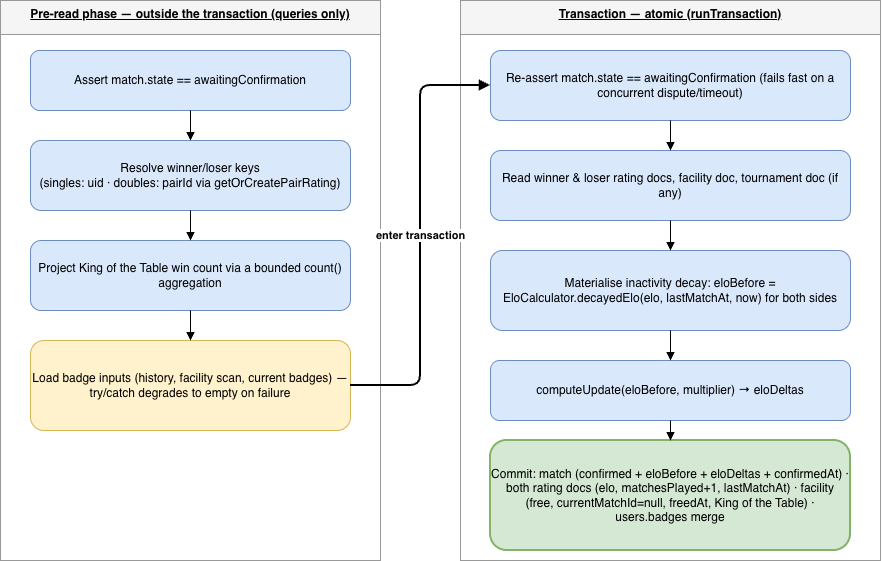
\includegraphics[width=0.9\textwidth]{diagrams/confirm_txn}
    \caption{The atomic match-confirmation flow.}
    \label{fig:confirm_txn}
\end{figure}

Three details matter. First, the state guard is asserted twice: once in the pre-read for a fast failure, and again inside the transaction so a concurrent dispute or timeout cannot race the confirmation. Second, the lazy inactivity decay is materialised at this moment — \texttt{EloCalculator.decayedElo} is applied to both stored ratings before the exchange is computed, so a returning player's decayed value becomes their real \texttt{eloBefore}. Third, achievement evaluation is deliberately failure-tolerant: badge inputs are gathered in a \texttt{try/catch} that degrades to empty inputs, because a cosmetic subsystem must never be able to abort a competitive write. On commit, one transaction writes: the match ($\rightarrow$ \texttt{confirmed} + \texttt{eloBefore} + \texttt{eloDeltas} + \texttt{confirmedAt}), both rating documents ($\rightarrow$ \texttt{elo}, \texttt{matchesPlayed}+1, \texttt{lastMatchAt}), the facility ($\rightarrow$ \texttt{free}, \texttt{currentMatchId} null, \texttt{freedAt}, King of the Table if the projected wins exceed the current), and the merged \texttt{users/\{uid\}.badges} for newly earned achievements.

The dispute path reuses the same machinery. A genuine dispute increments \texttt{disputeCount}, frees the facility, and leaves ratings untouched; the third dispute sets a 7-day \texttt{disputePenaltyUntil} and resets the counter. If a penalised player attempts to dispute during the cooldown, the transaction silently forces the match to \texttt{confirmed} and applies the normal ELO writes, protecting the rating economy from serial griefers without a moderation backend.

\section{Runtime View: Queue Join and Check-in}
\label{sec:queue_txn}
The queue is the flow most exposed to concurrent writers. Joining is a transaction: if the caller's own ticket exists it is returned (idempotent); otherwise the facility's \texttt{queueTailPosition} is read, \texttt{position = tail + 1} is claimed, the queue document is written, and \texttt{queueTailPosition} is bumped. Every watcher recomputes a dense display rank from snapshot order, not from stored positions.

\begin{figure}[H]
    \centering
    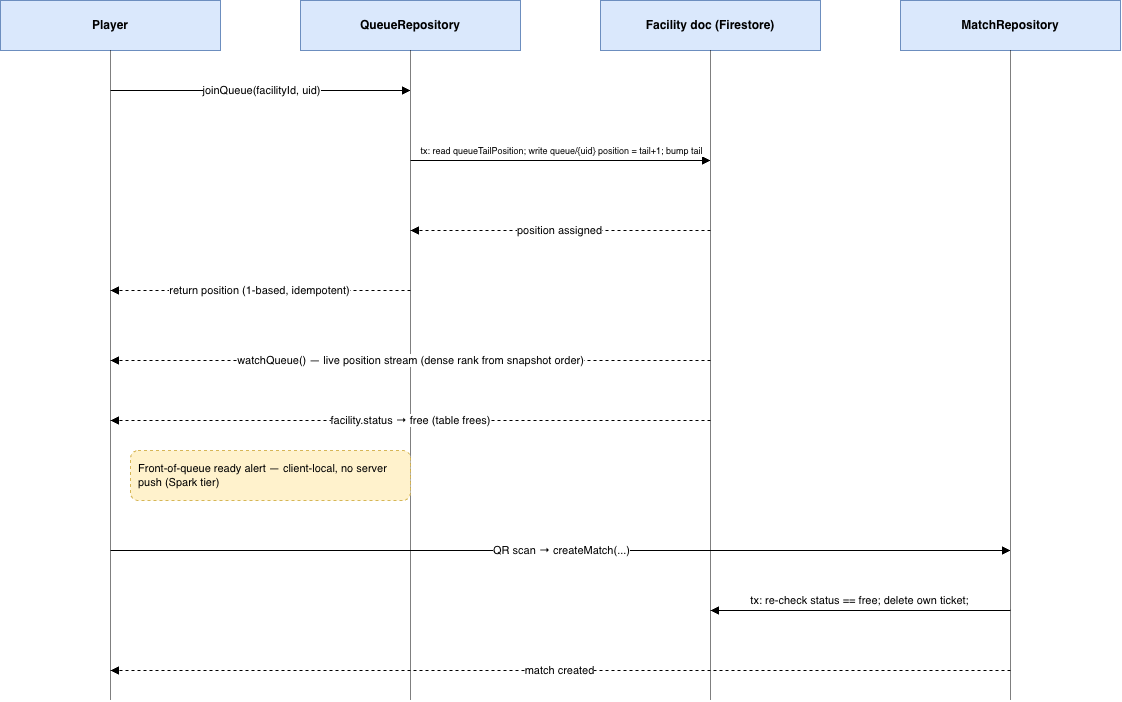
\includegraphics[width=0.9\textwidth]{diagrams/queue_sequence}
    \caption{Queue-join and Proof-of-Play check-in sequence.}
    \label{fig:queue_sequence}
\end{figure}

Queue enforcement is deliberately \emph{soft}: a non-front player who scans first sees a ``someone is ahead of you'' warning dialog rather than a hard block, because the physical table, not the app, is the real arbiter. When the table frees, the front player's own listener detects \texttt{status $\rightarrow$ free} and raises a client-local ready alert (no server push on the Spark tier).

\section{Modular Navigation and Deep Linking}
\label{sec:navigation}
Routing uses \texttt{go\_router} with a \texttt{StatefulShellRoute.indexedStack}, so each of the four tabs keeps its own navigation stack. The custom \texttt{campusarena://} scheme is rewritten inside the top-level redirect (\texttt{campusarena://play/facility/x} is rebuilt to \texttt{/play/facility/x} and re-evaluated). Deep-link targets that arrive while signed out (\texttt{/play/facility/:id} from a QR sticker, \texttt{/challenge/:id} from a notification) are stashed in a \texttt{pendingDeepLink} and delivered exactly once after authentication and onboarding. The router's single redirect function enforces the whole auth gate: unauthenticated users are bounced to \texttt{/landing}, authenticated users with \texttt{onboardingComplete == false} are forced into \texttt{/onboarding/tutorial}, ready users are kept out of auth screens, and the splash holds while the user document loads. Because \texttt{GoRouterRefreshStream} notifies on every Cubit emission, the guard re-evaluates the moment auth state changes. Transient surfaces (dialogs, sheets) use the imperative \texttt{Navigator}.

\section{Arena Assistant}
\label{sec:assistant_arch}
The Arena Assistant is a read-only, in-app natural-language assistant on a full-screen \texttt{/chatbot} route. Its data path is deliberately narrow.

\begin{itemize}
    \item \textbf{Read-only tool layer.} \texttt{ChatbotToolsService} exposes bounded, one-shot tools built on the existing repositories: \texttt{getEmptyTables}, \texttt{getFacilitiesByStatus}, \texttt{getTournamentsToday}, \texttt{getUserQueuePosition}, \texttt{getUserEloAndRank}, and the static \texttt{explainHowEloWorks}. Every query carries a \texttt{.limit()} of at most 25, uses single-shot reads (no listeners), and never writes. The chatbot adds zero collections, zero Security-Rules surface, and negligible quota; conversation history is session-only Cubit state, never persisted.
    \item \textbf{Orchestration (classify-then-ground, not function calling).}\\ \texttt{ChatbotRepository.answer} first classifies the message with \texttt{RuleBasedIntentMatcher}, a deterministic keyword matcher covering English and Italian phrasings (\texttt{emptyTables}, \texttt{tournamentsToday}, \texttt{eloExplainer}, \texttt{queuePosition}, \texttt{general}). The matching tool runs first, and its results are injected into the system prompt as grounding context; only then is a single LLM call made through \texttt{LlmClient} (temperature 0.2, bounded tokens, 45-second timeout). The model never chooses which query to run and never sees raw database access — it only phrases an answer over data the app already fetched. This shape was chosen over a native function-calling loop because it is deterministic, cheaper (one call per turn), and keeps the grounding guarantee in code rather than in a prompt.
    \item \textbf{Provider.} \texttt{LlmClient} speaks to five OpenAI-compatible or vendor-specific endpoints (\texttt{regolo}, \texttt{openai}, \texttt{openrouter}, \texttt{anthropic}, \texttt{gemini}). The shipped default is \textbf{Regolo}, an EU-hosted inference platform with a free tier, using \texttt{qwen3.5-122b}. Provider, key, and model are wired at build time through \texttt{-{}-dart-define} values (\texttt{ASSISTANT\_PROVIDER}, \texttt{ASSISTANT\_API\_KEY}, \texttt{ASSISTANT\_MODEL}) and can be overridden from a settings screen, persisted via \texttt{shared\_preferences}.
    \item \textbf{Fallback and disclaimer.} When no key is configured, the device is offline, or the LLM call fails, the assistant degrades to ``limited mode'': the same tool results are rendered through templated, localised answers from the intent matcher. Two rules are enforced in code, not delegated to the model: availability answers always carry the mandatory disclaimer (availability reflects app activity only; a table shown as free may be in use by non-app players; CampusArena is not a reservation service), appended whenever an availability tool fired; and the first-open banner shows the full disclaimer copy. A short disclaimer, worded per surface, appears on facility detail cards and in the tutorial's map step.
\end{itemize}

\section{External Services Integration}
\label{sec:external_services}

Beyond the Firebase suite (Auth, Firestore, FCM), CampusArena consumes \textbf{five external integrations} with real interaction rather than storage alone.

\subsection{Open-Meteo (Weather)}
\texttt{WeatherRepository} calls the free, keyless Open-Meteo REST API at \texttt{api.open-meteo.com}\slash\allowbreak\texttt{v1}\slash\allowbreak\texttt{forecast} through \texttt{Uri.https}, requesting \texttt{temperature\_2m}, \texttt{precipitation}, \texttt{wind\_speed\_10m}, and \texttt{weather\_code}. Two operations are exposed: \texttt{getCurrentWeather} returning a \texttt{WeatherSnapshot} in metric units, and \texttt{getHourlyForecast} with a bounded window (default 4 hours) for tournament timeslots. Weather is decorative by policy: it appears only on \texttt{isOutdoor} facility cards and outdoor-tournament forecasts, any non-200 or parse failure surfaces as a silent omission rather than an error screen, and results are cached in memory by \texttt{WeatherCubit}. Nothing weather-related is persisted.

\subsection{OpenStreetMap Tiles with Persistent Caching}
The map renders OpenStreetMap raster tiles through \texttt{flutter\_map}. The OSM tile-usage policy requires clients to honour HTTP caching, so \texttt{buildOsmTileProvider} wraps the network fetch in a \texttt{CachedTileProvider} from \texttt{flutter\_map\_cache} backed by a \texttt{DriftCacheStore} (an on-disk SQLite store in the app cache directory). The store honours \texttt{Cache-Control}/\texttt{Expires} headers and falls back to a \texttt{maxStale} of 30 days, comfortably above the policy's 7-day minimum. Construction is best-effort: if the store cannot be created the function returns \texttt{null} and the map falls back to the default in-memory provider, so a cache failure can never take the map down. The required attribution links through to the OSM licence page.

\subsection{Regolo LLM (Arena Assistant)}
The assistant's LLM path is described in \cref{sec:assistant_arch}: a single, grounded call to the Regolo endpoint (\texttt{https://api.regolo.ai}\slash\allowbreak\texttt{v1}\slash\allowbreak\texttt{chat}\slash\allowbreak\texttt{completions}) by default, with four other supported providers, and a deterministic rule-based fallback whenever the call cannot be made. The two hardware integrations — \texttt{mobile\_scanner} for QR check-in and \texttt{geolocator} for the soft GPS audit — are covered in the Proof-of-Play requirement (\cref{sec:functional_requirements}).

\section{Other Significant Decisions}
\begin{itemize}
    \item \textbf{Single design language.} Material 3 across both platforms, themed from one seed colour, rather than a platform-adaptive Cupertino variant — one look to polish, one to test.
    \item \textbf{Cubit over Riverpod/Provider.} With the BLoC event layer already dropped (\cref{sec:high_level_overview}), Cubit won on the team's coursework familiarity and direct testability with \texttt{bloc\_test}.
\end{itemize}

% ============================================================
%   CHAPTER 5 — USER INTERFACE (UI/UX)
% ============================================================

\chapter{User Interface (UI/UX)}
\label{ch:user_interface}

\section{Design Guidelines}
The interface follows \textbf{Material Design 3} with a single seeded colour scheme, rendered consistently in both light and dark themes; every surface sources \texttt{ColorScheme} roles rather than hardcoded colours. The UI is fully internationalised in English and Italian; only UI chrome is translated, never player names or ELO values. Component states — default, loading, empty, and error — are designed explicitly. The renders in this chapter are exports of the project's implemented, interactive HTML/CSS design system (\cref{sec:design_system}).

\section{Navigation Map}
After authentication and first-launch onboarding, the app opens on a four-tab shell built with \texttt{StatefulShellRoute.indexedStack}, so each tab keeps its own navigation stack and scroll state. Full-screen flows (match, result, tournaments, chatbot, friends, settings) are pushed on the root navigator above the shell.

\begin{figure}[H]
    \centering
    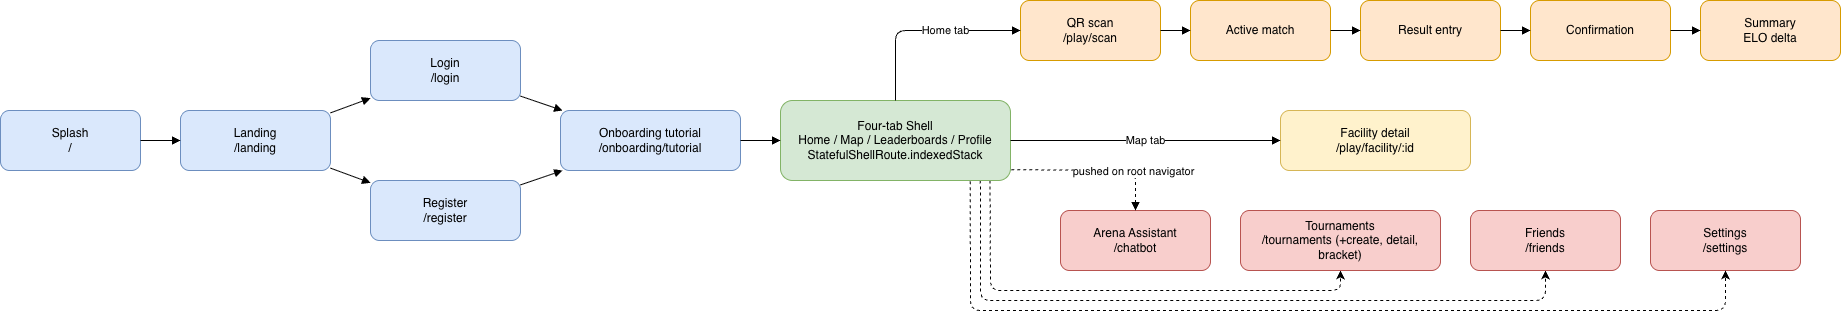
\includegraphics[width=\textwidth]{diagrams/navigation}
    \caption{Application navigation map.}
    \label{fig:navigation}
\end{figure}

\section{Screen Catalog}
\label{sec:screen_catalog}

\begin{figure}[H]
    \centering
    \subfloat[Splash]{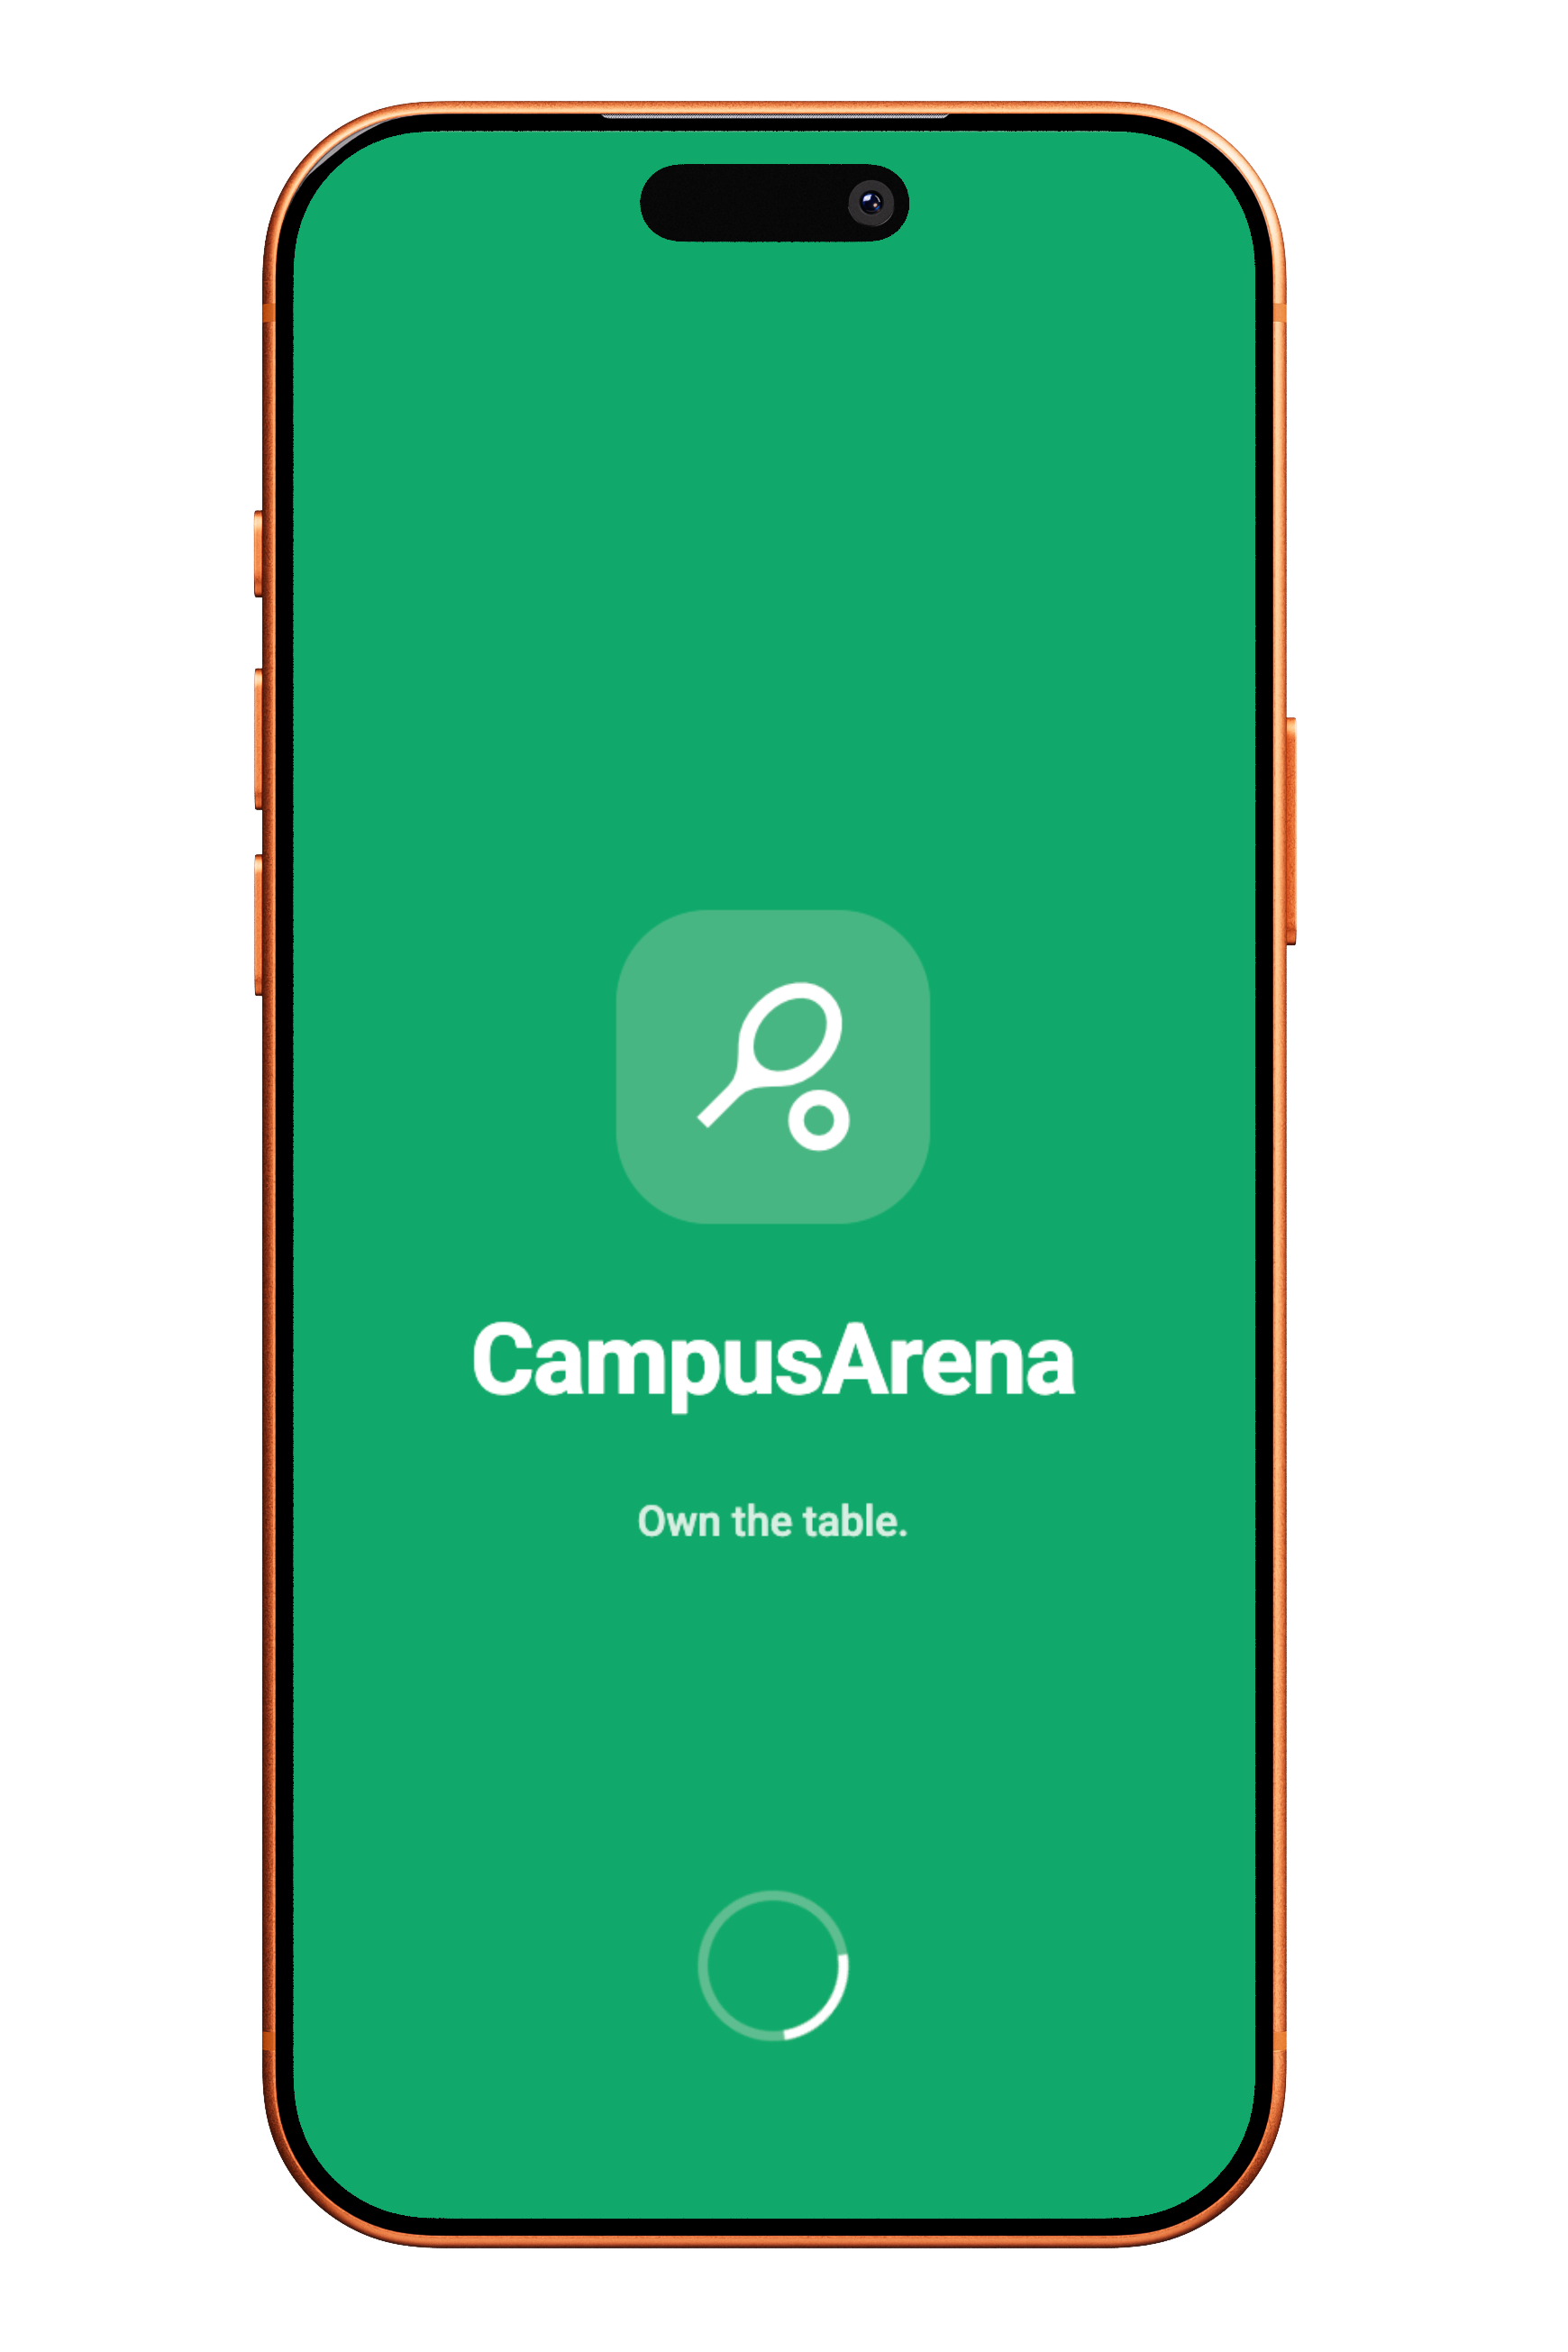
\includegraphics[width=0.20\linewidth]{mockups/splash_en_light}}\hfill
    \subfloat[Landing]{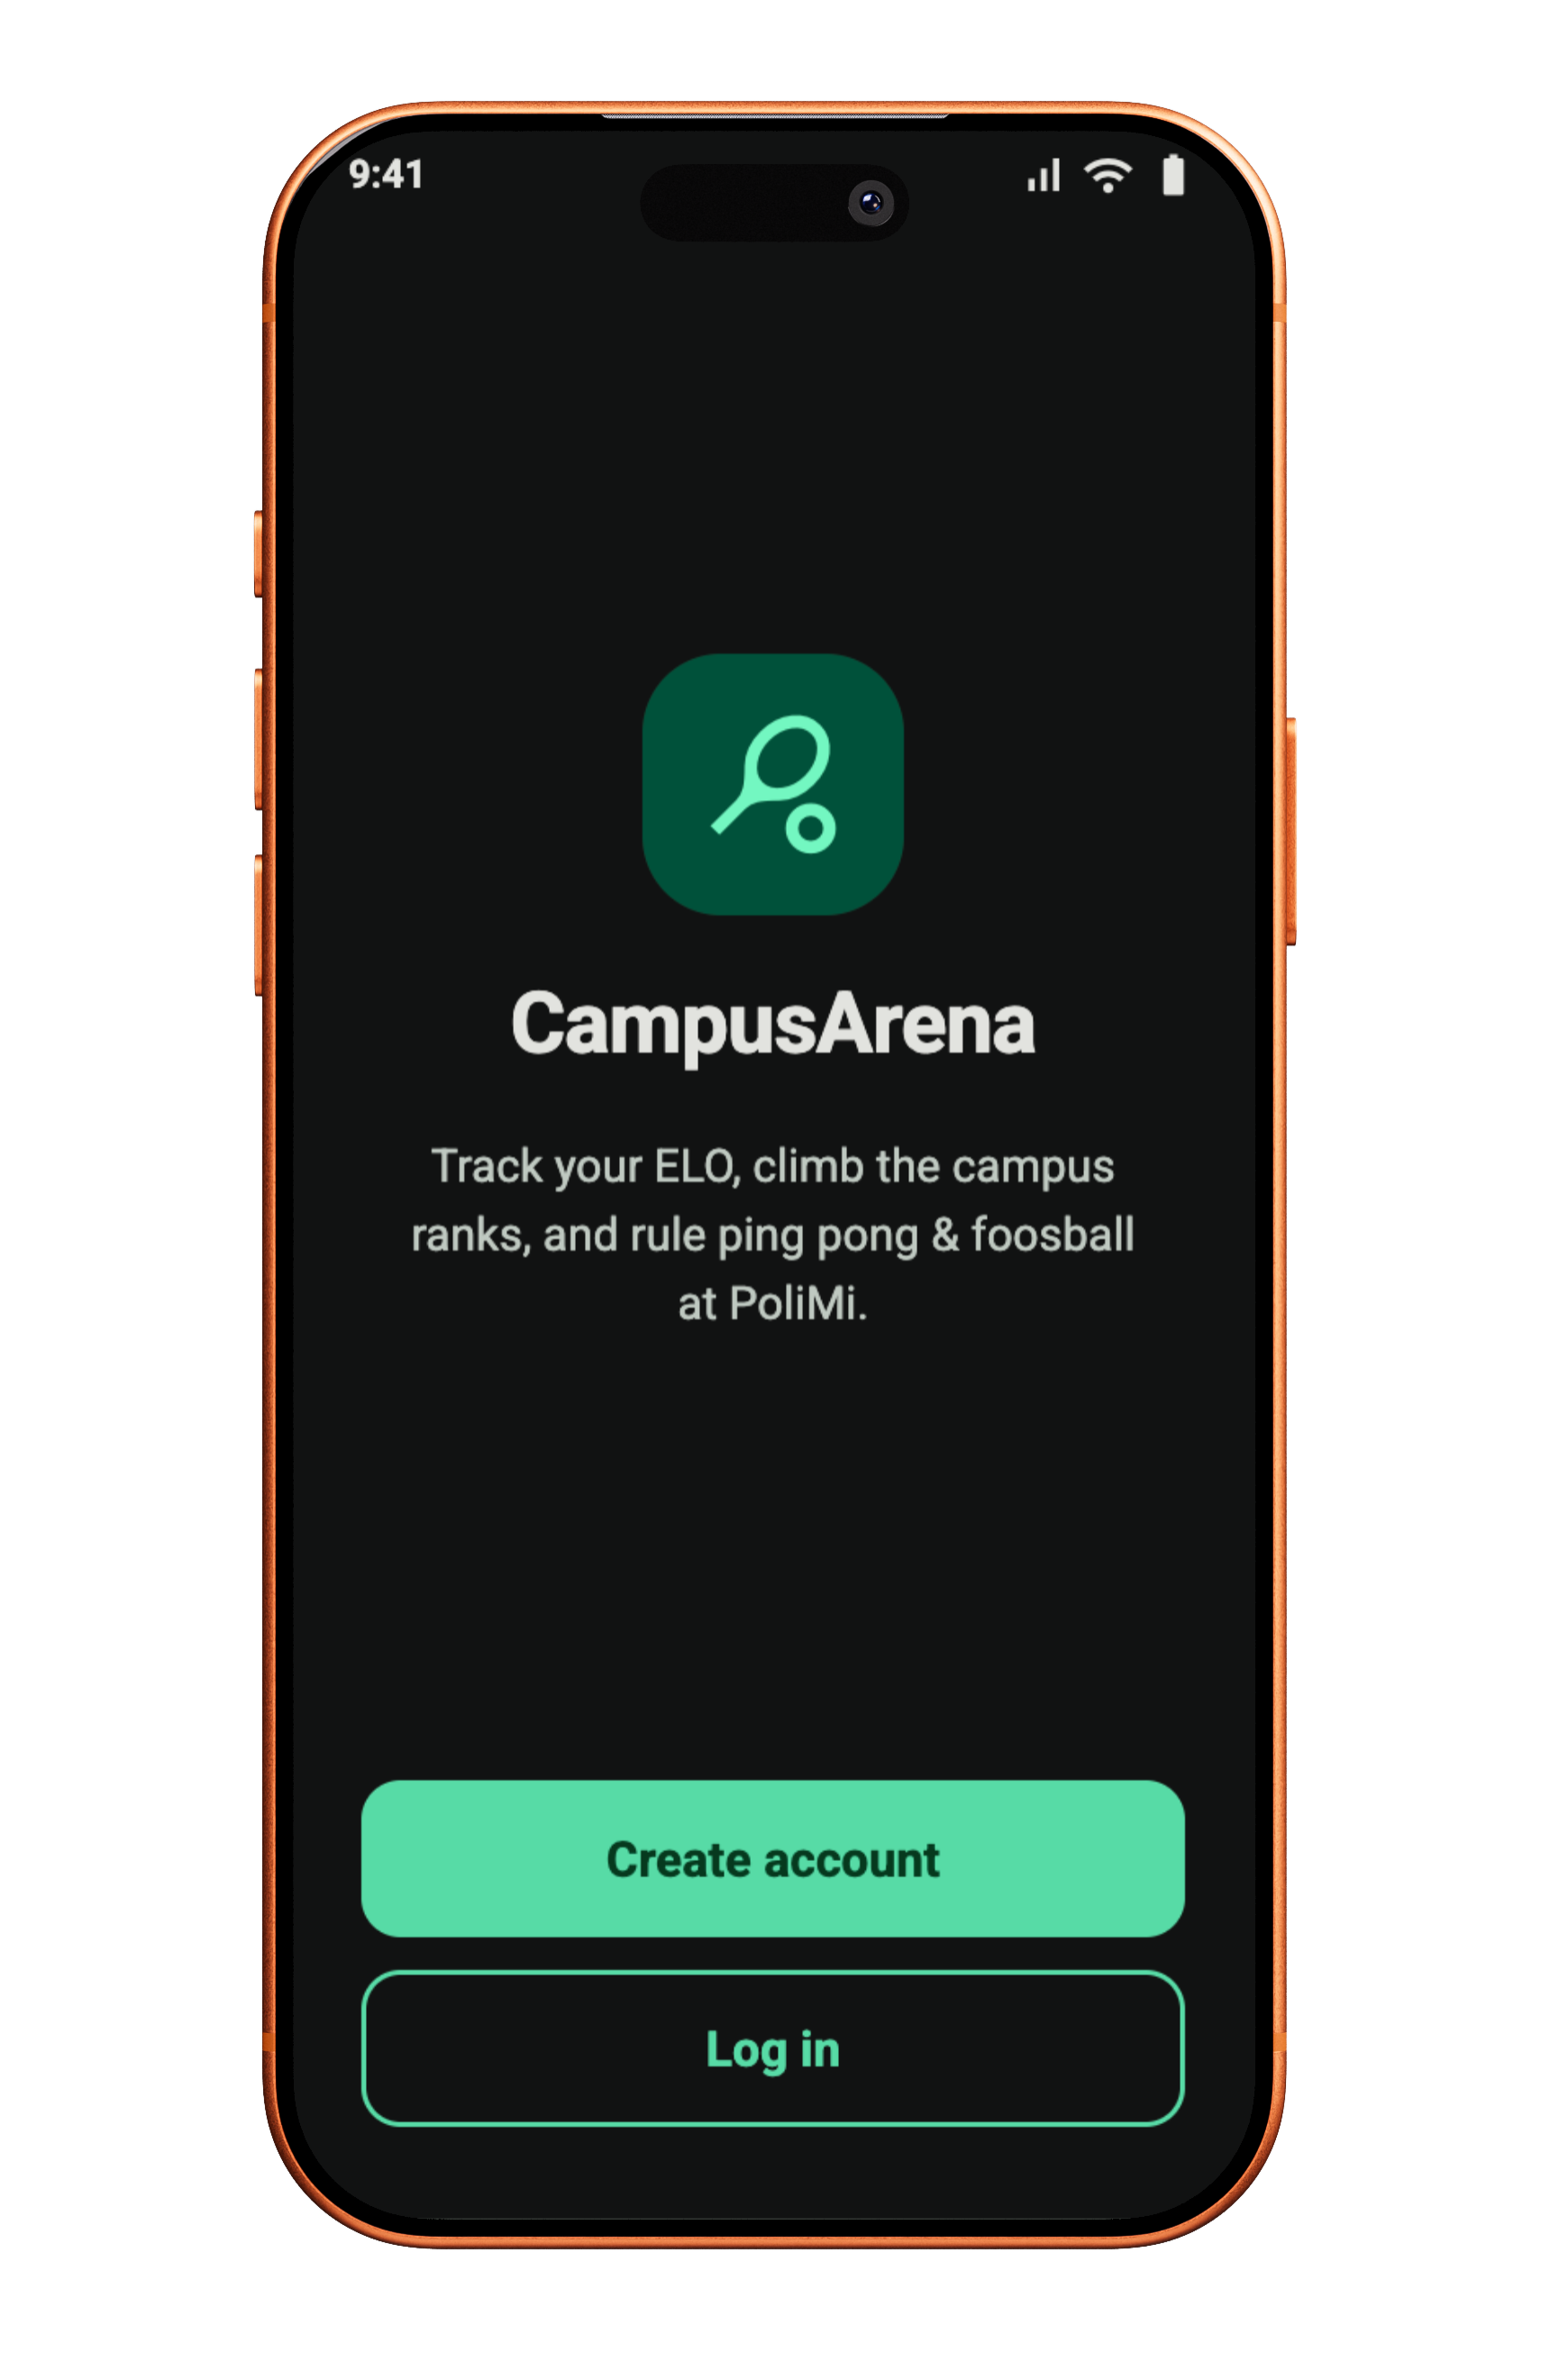
\includegraphics[width=0.20\linewidth]{mockups/landing_en_dark}}\hfill
    \subfloat[Login]{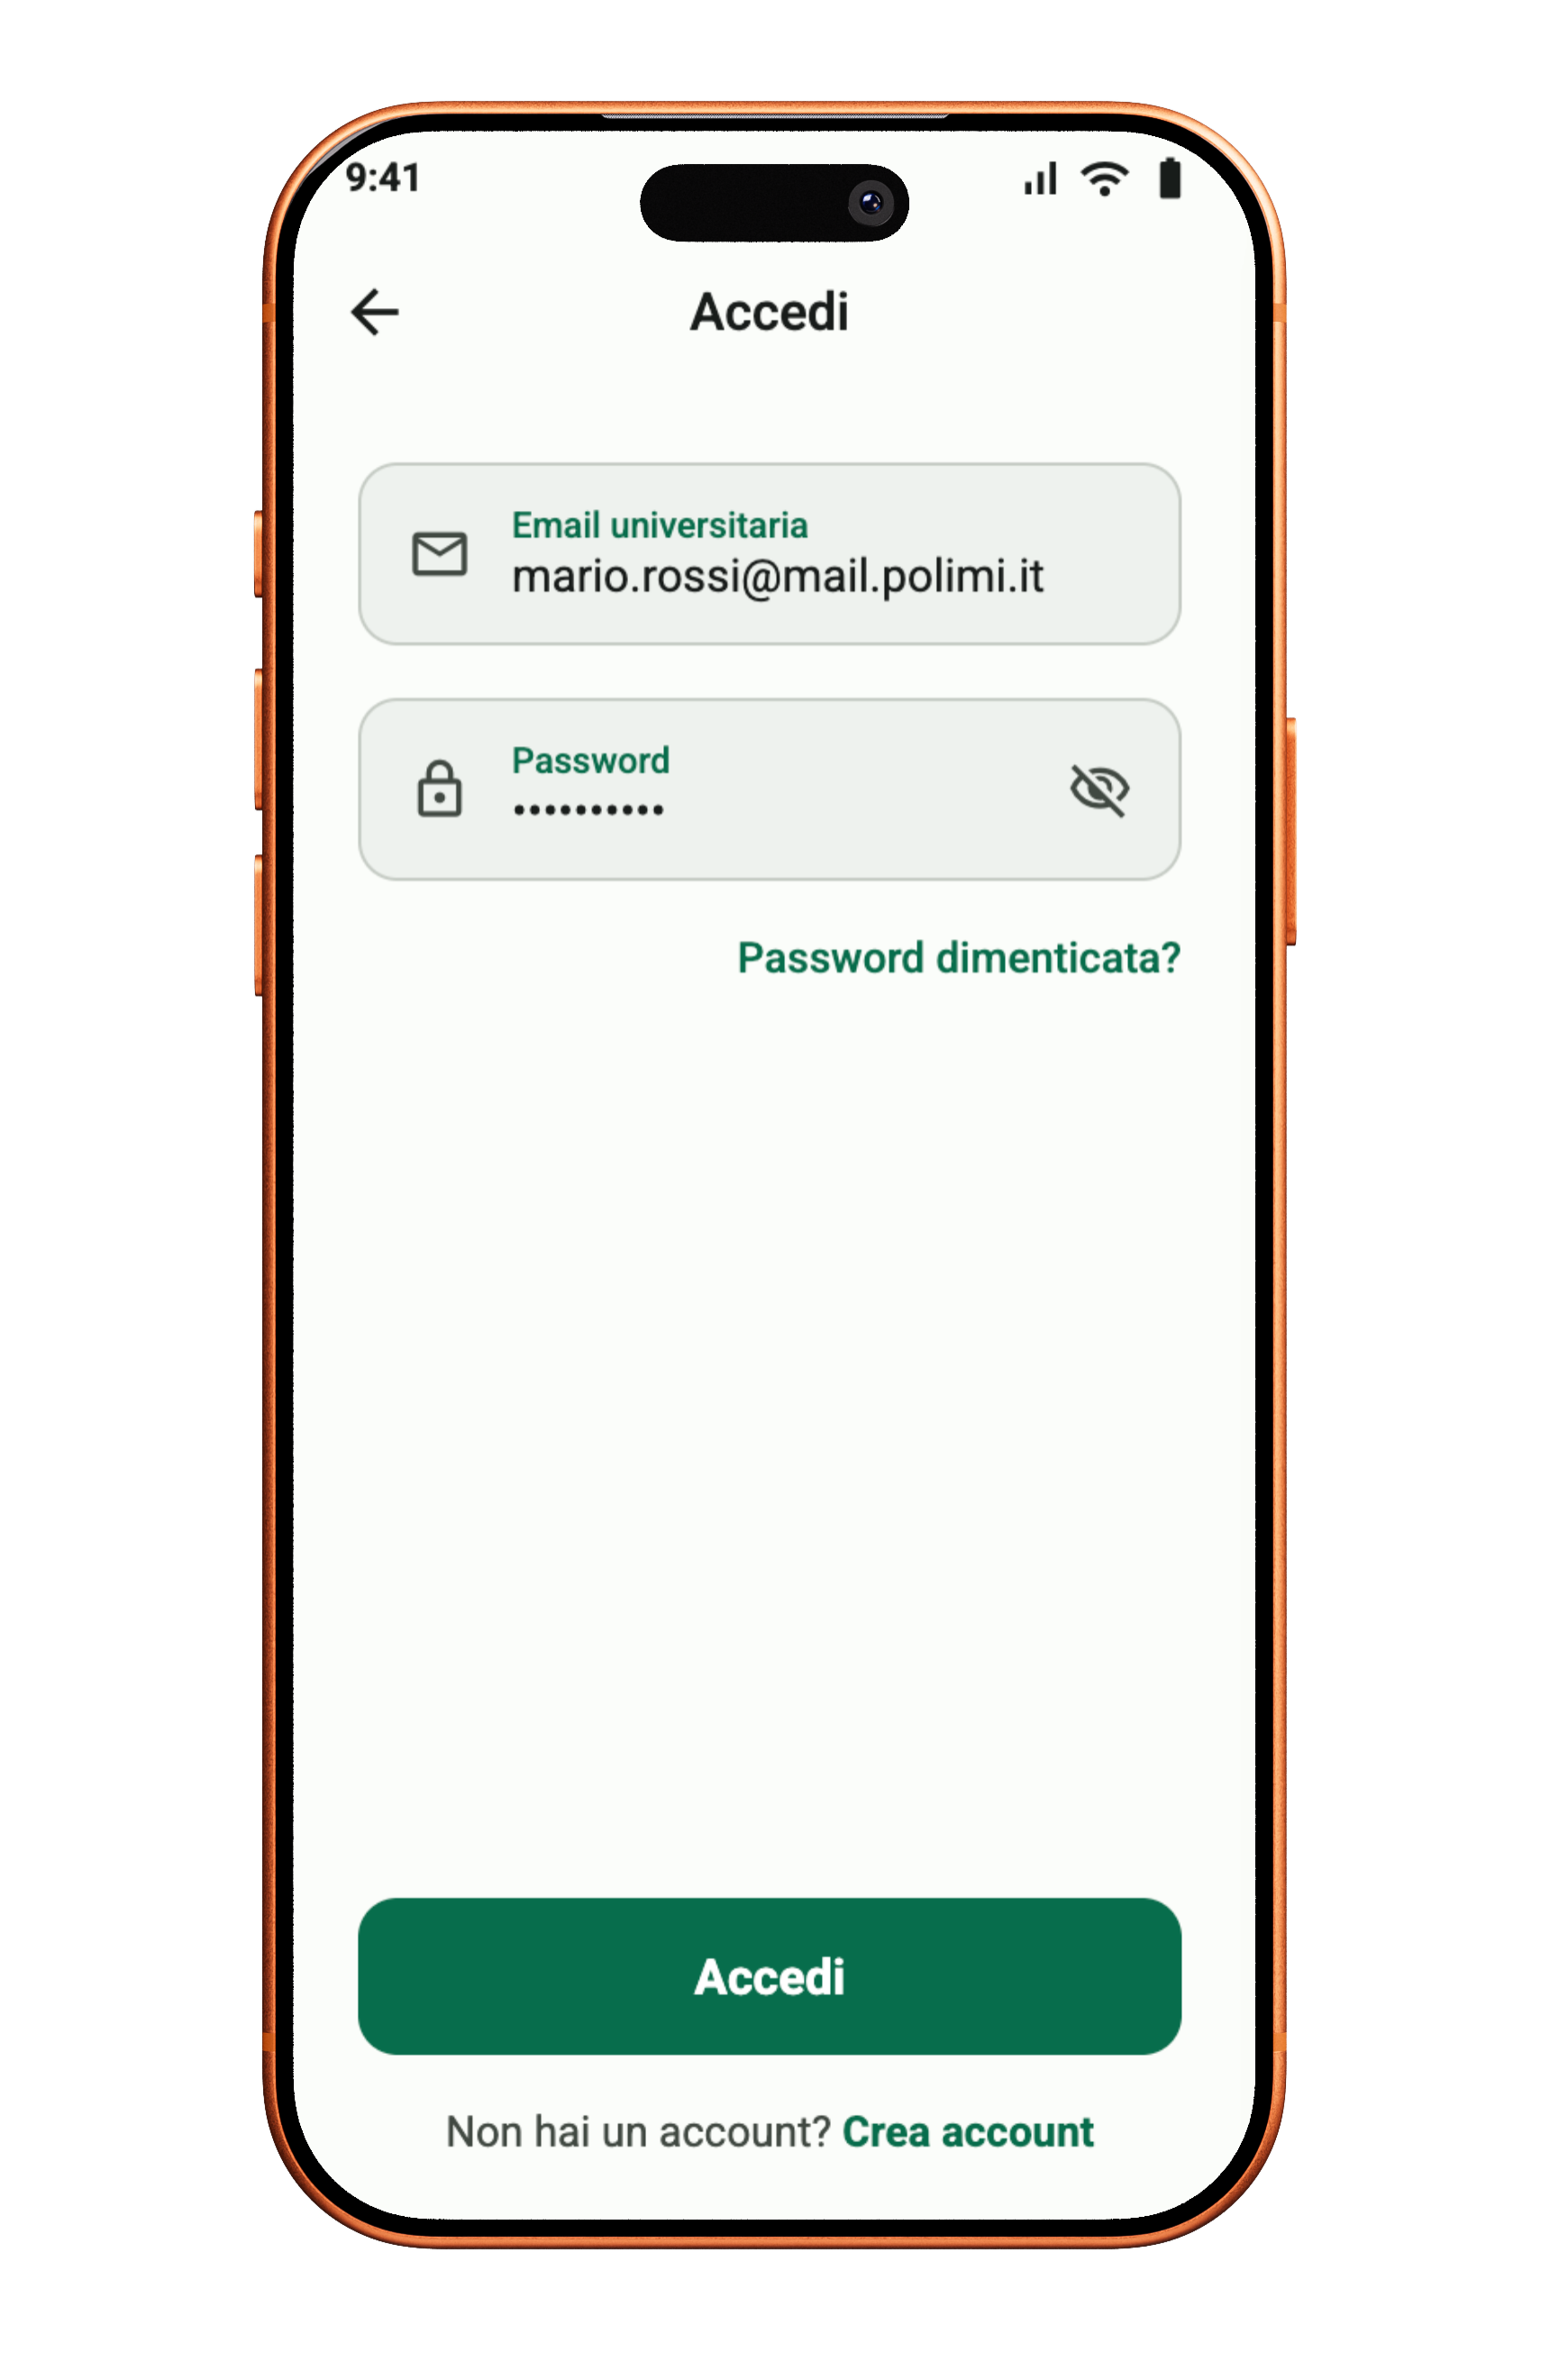
\includegraphics[width=0.20\linewidth]{mockups/login_it_light}}\hfill
    \subfloat[Register]{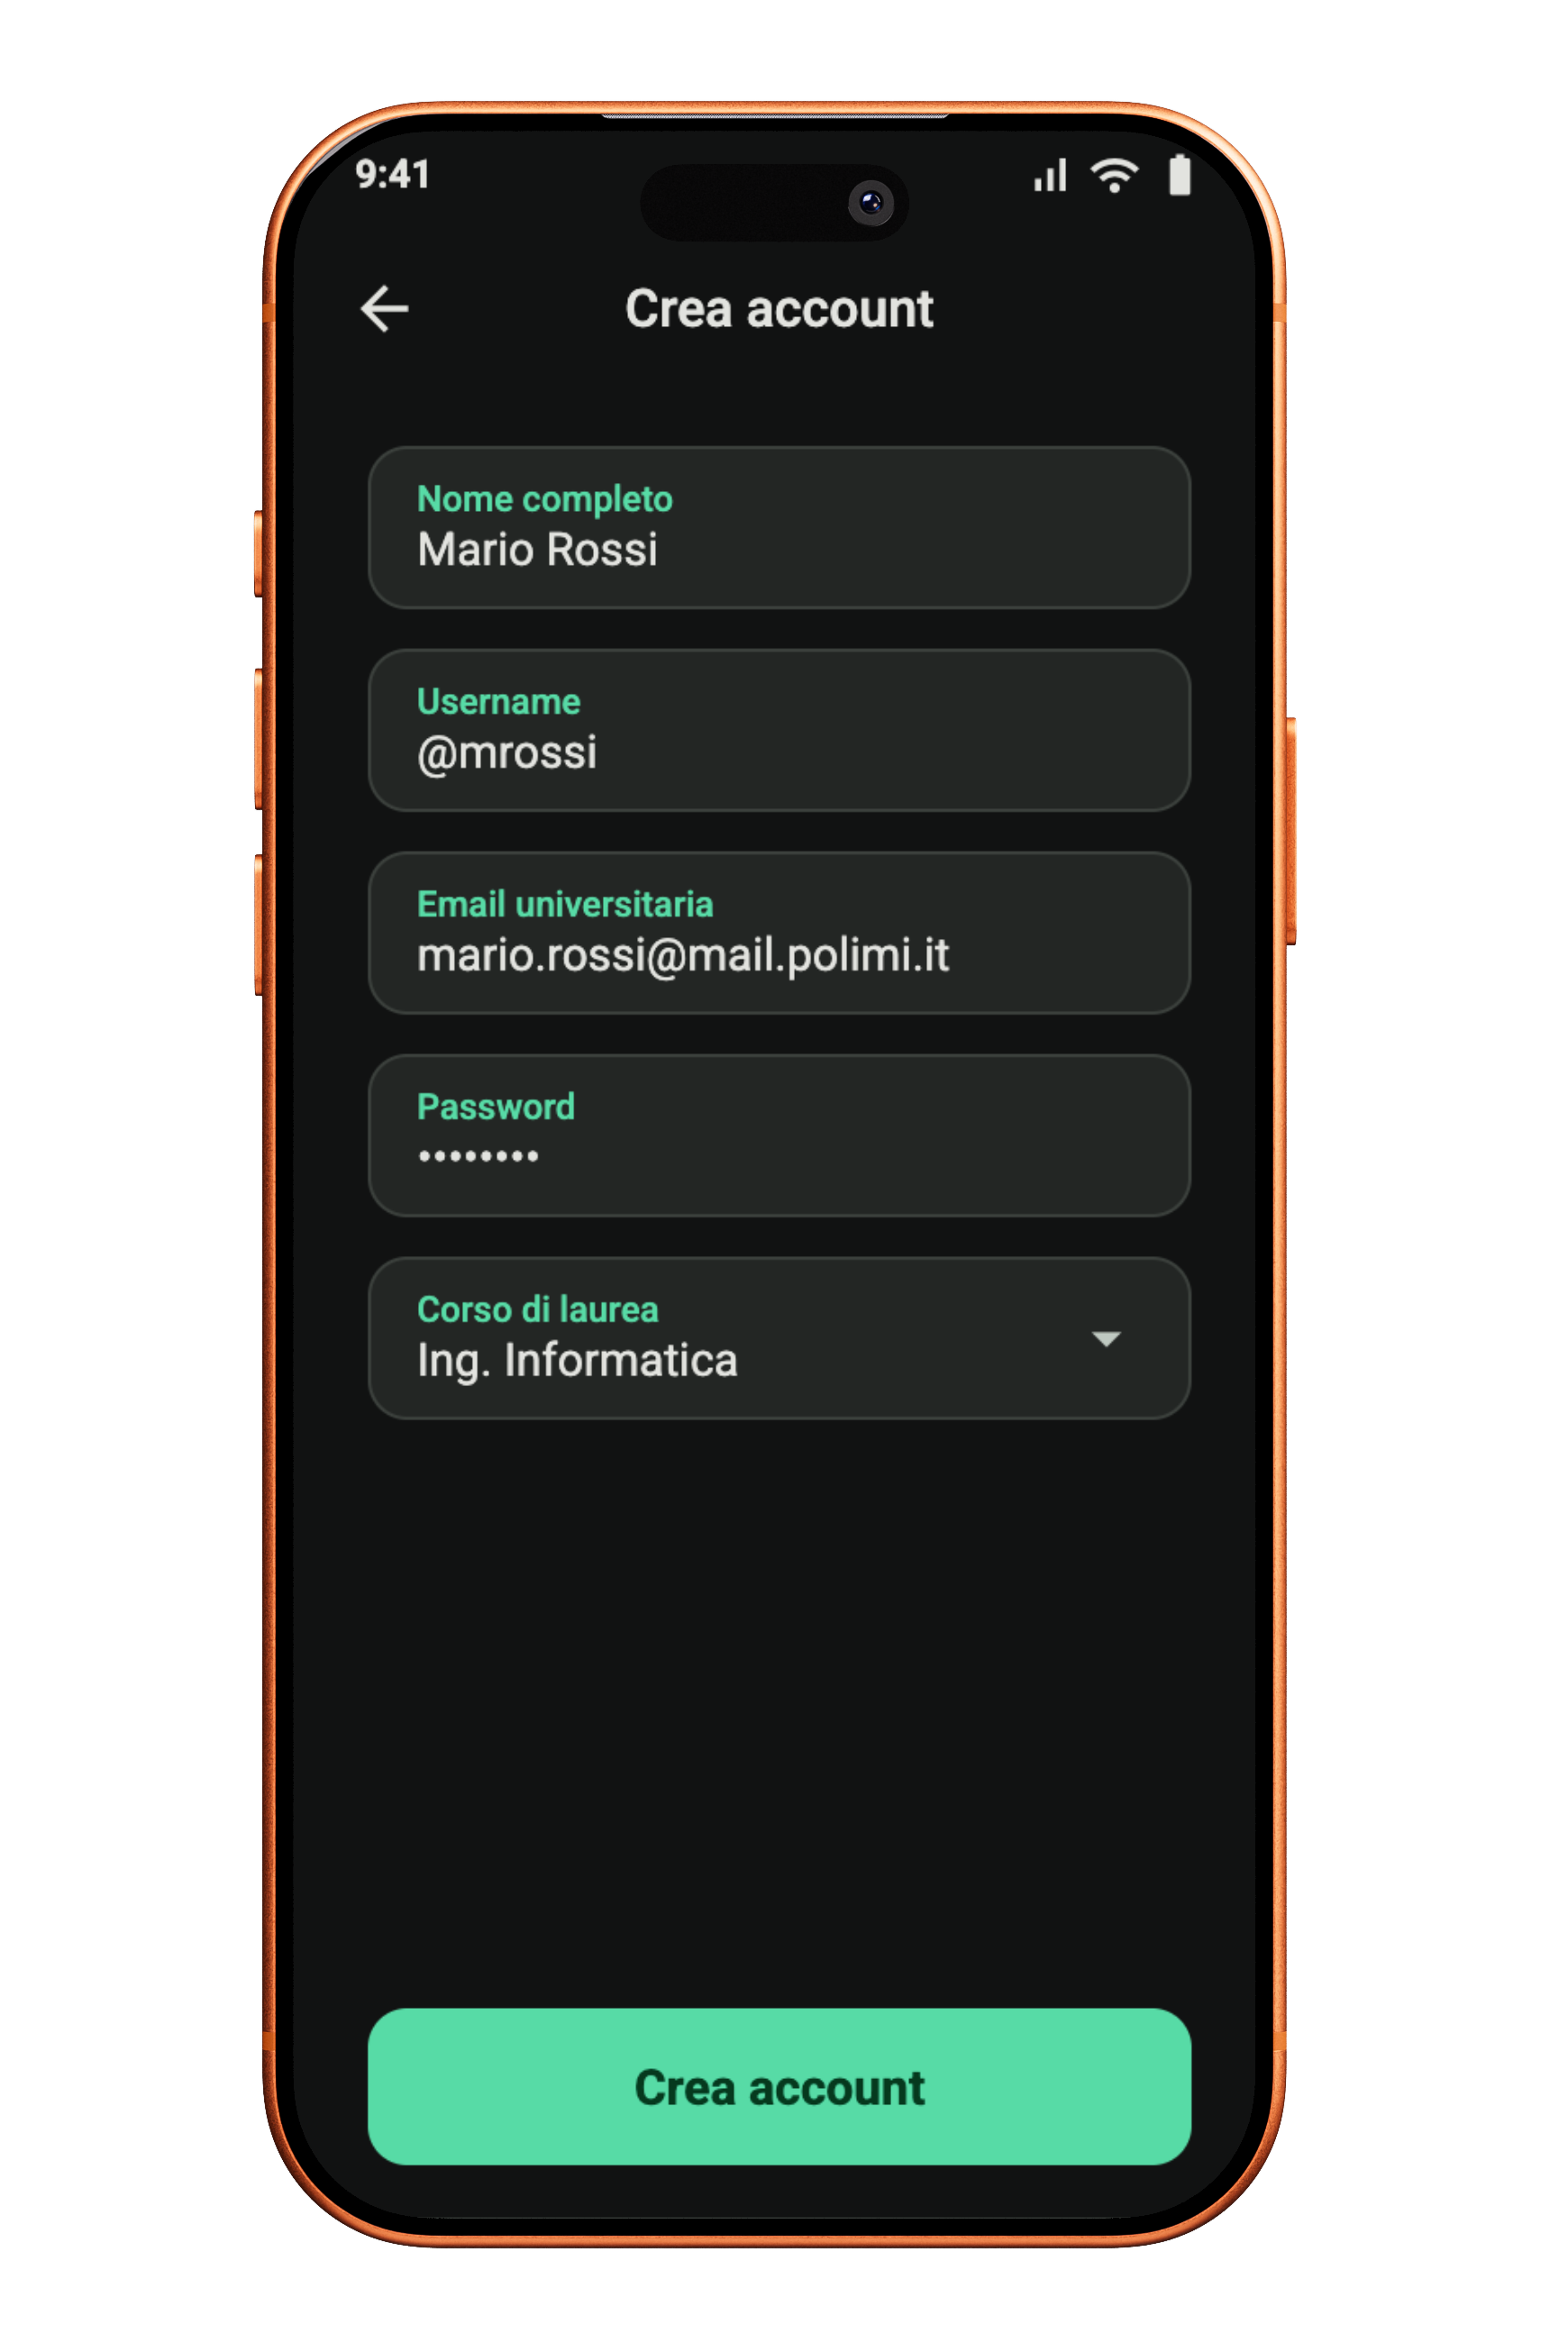
\includegraphics[width=0.20\linewidth]{mockups/registration_it_dark}}\hfill
    \subfloat[Mini-tutorial]{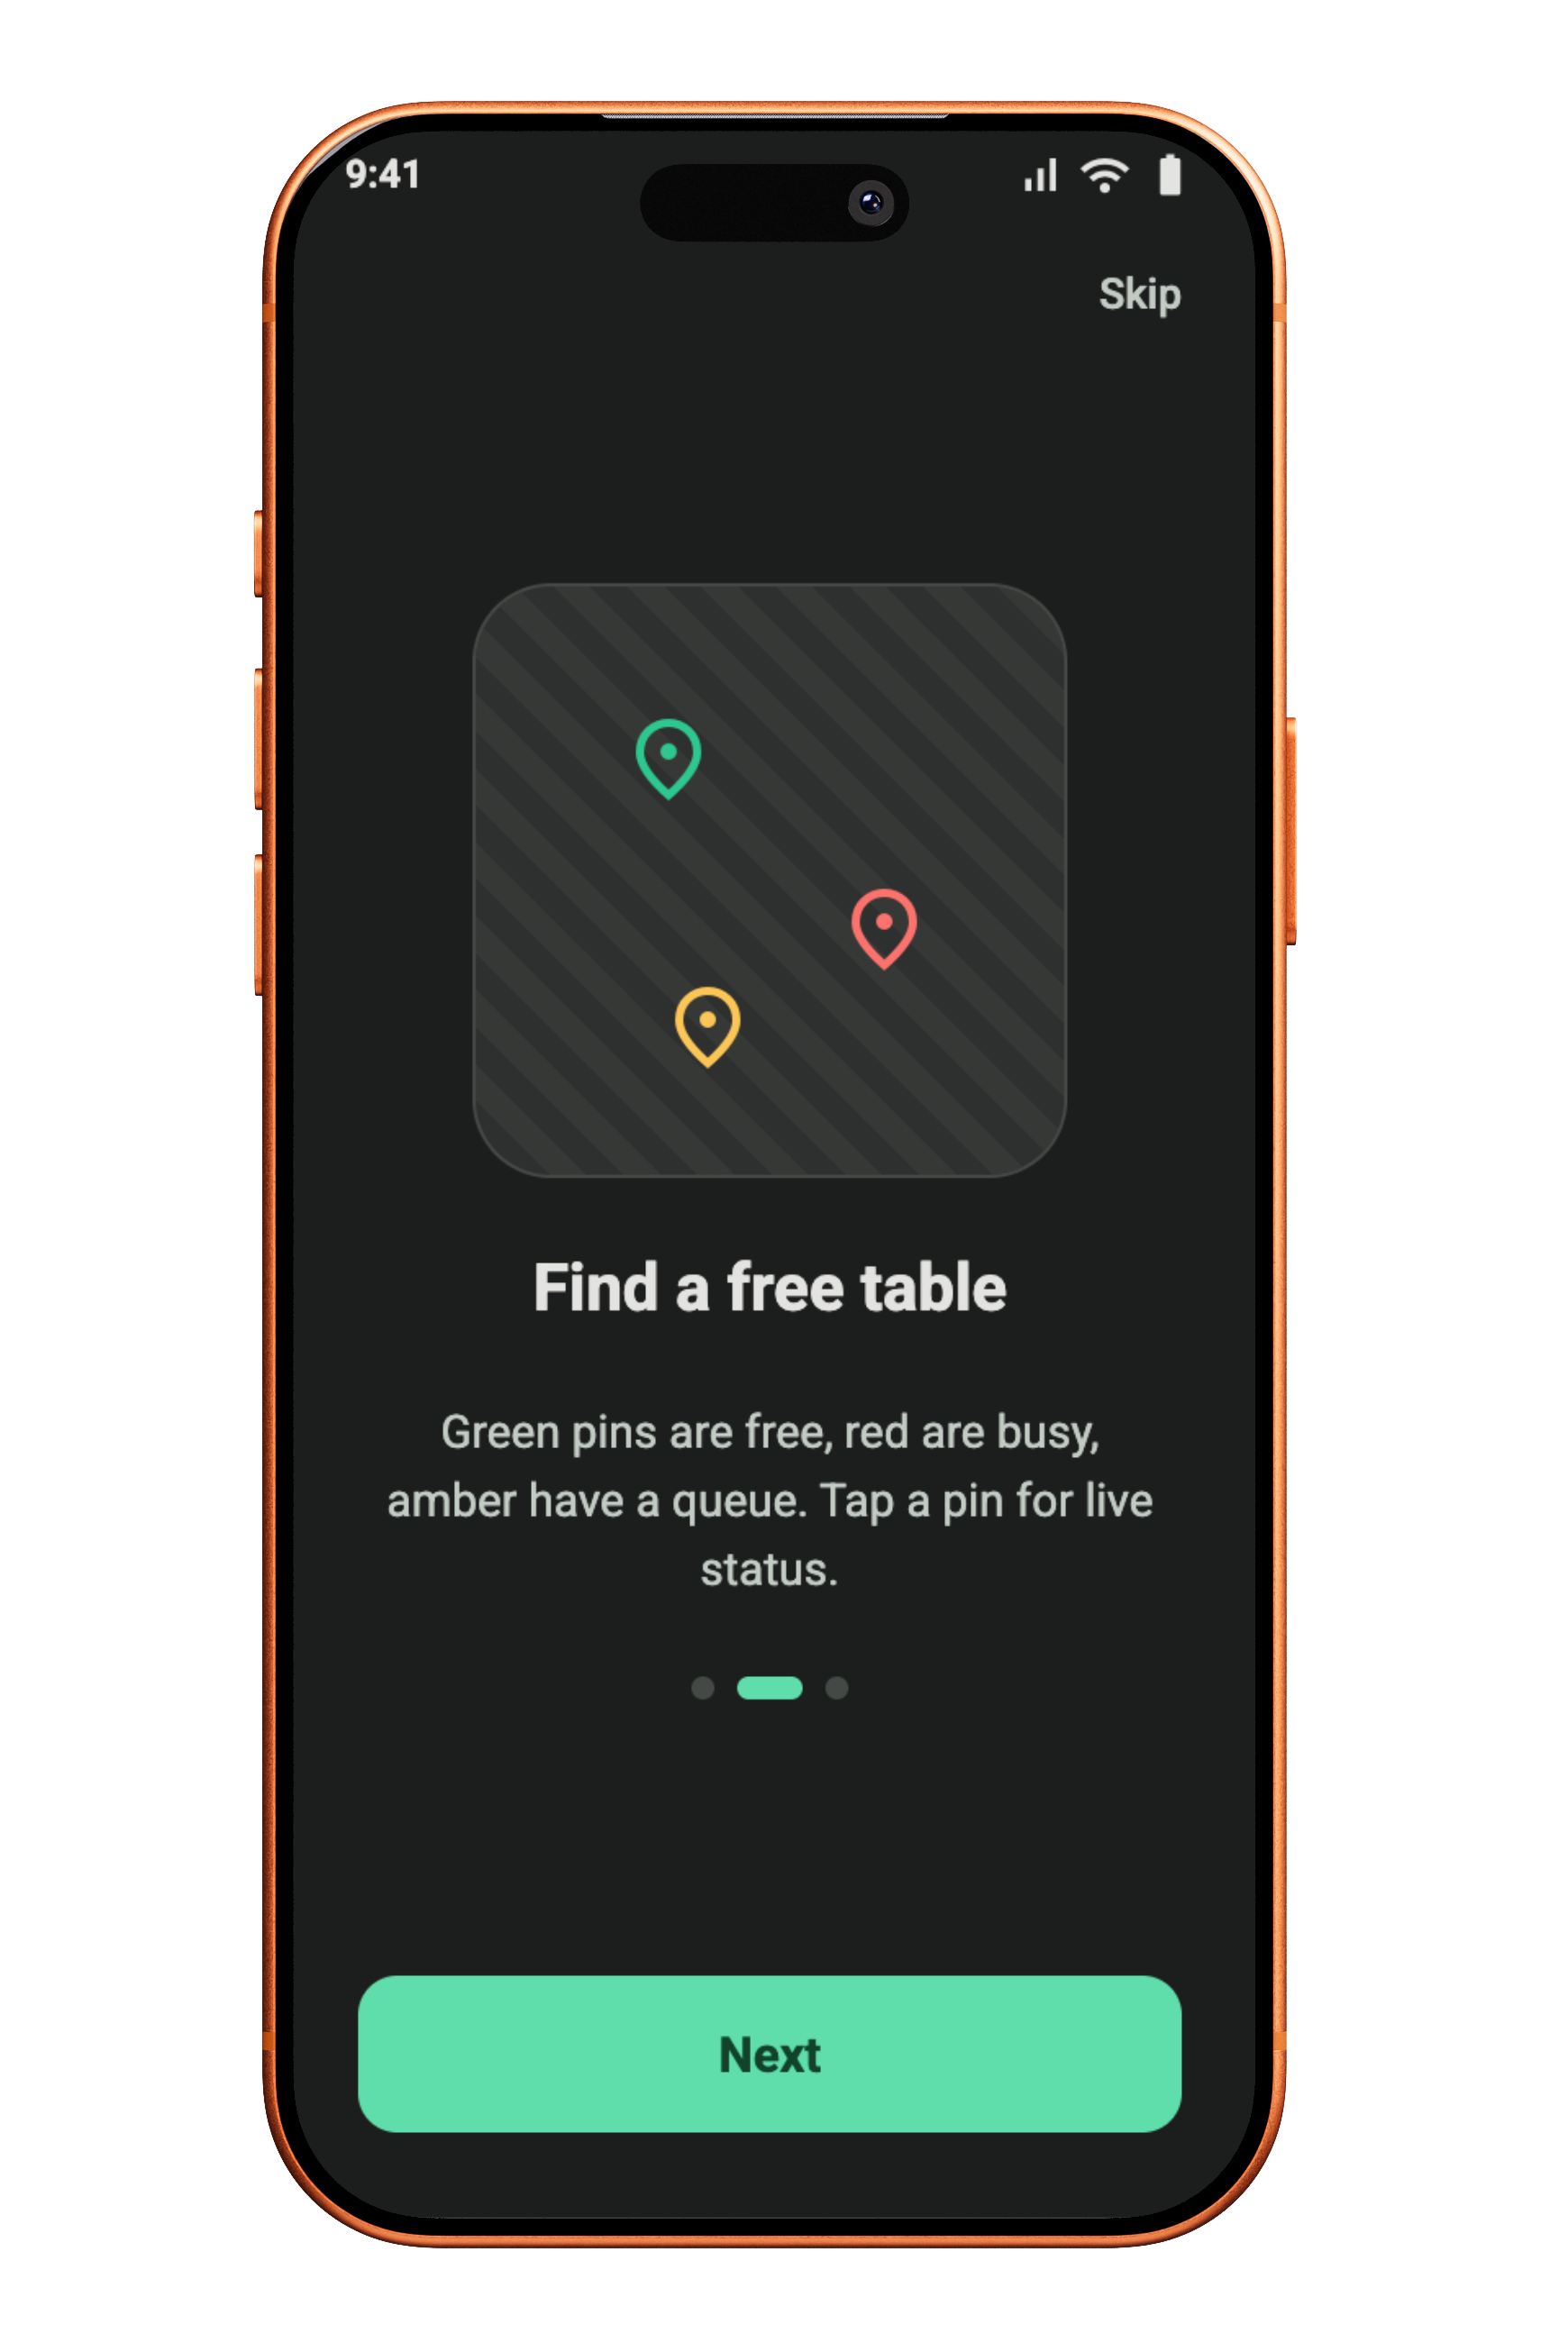
\includegraphics[width=0.20\linewidth]{mockups/tutorial_en_dark}}
    \caption{Authentication and onboarding screens.}
    \label{fig:auth_screens}
\end{figure}

\begin{figure}[H]
    \centering
    \subfloat[Home dashboard]{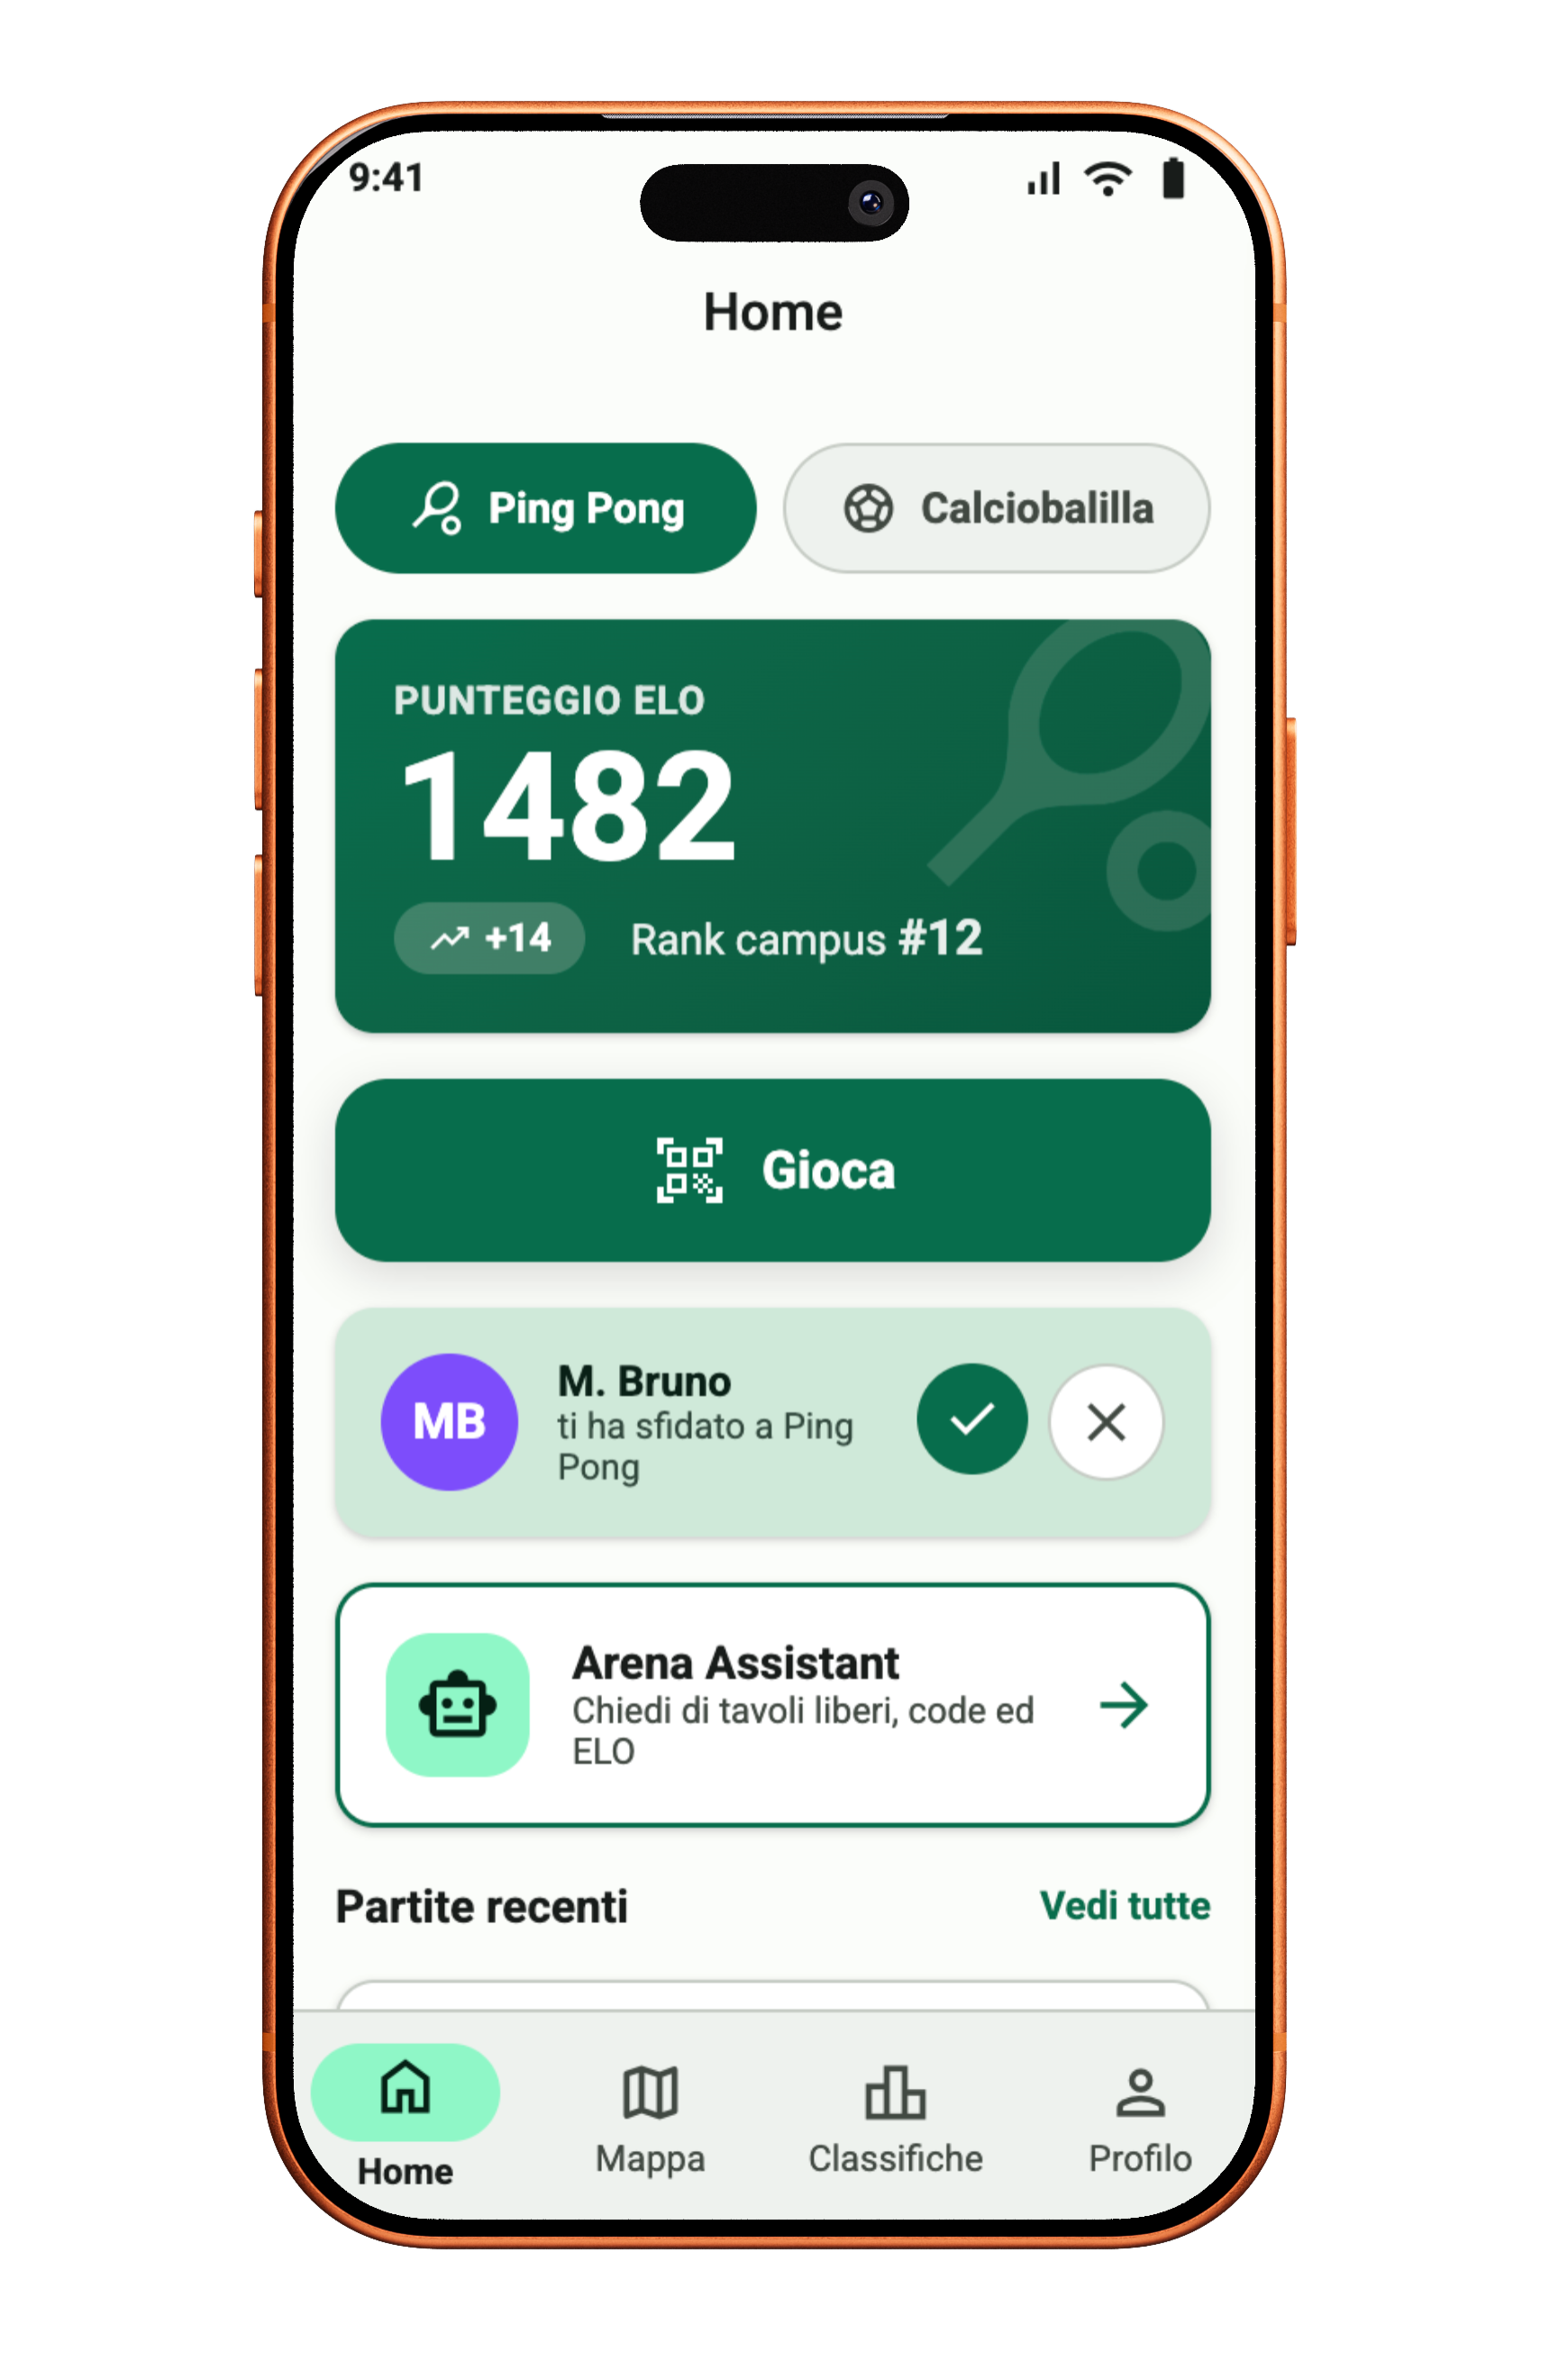
\includegraphics[width=0.25\linewidth]{mockups/home_it_light}}\hfill
    \subfloat[Map view]{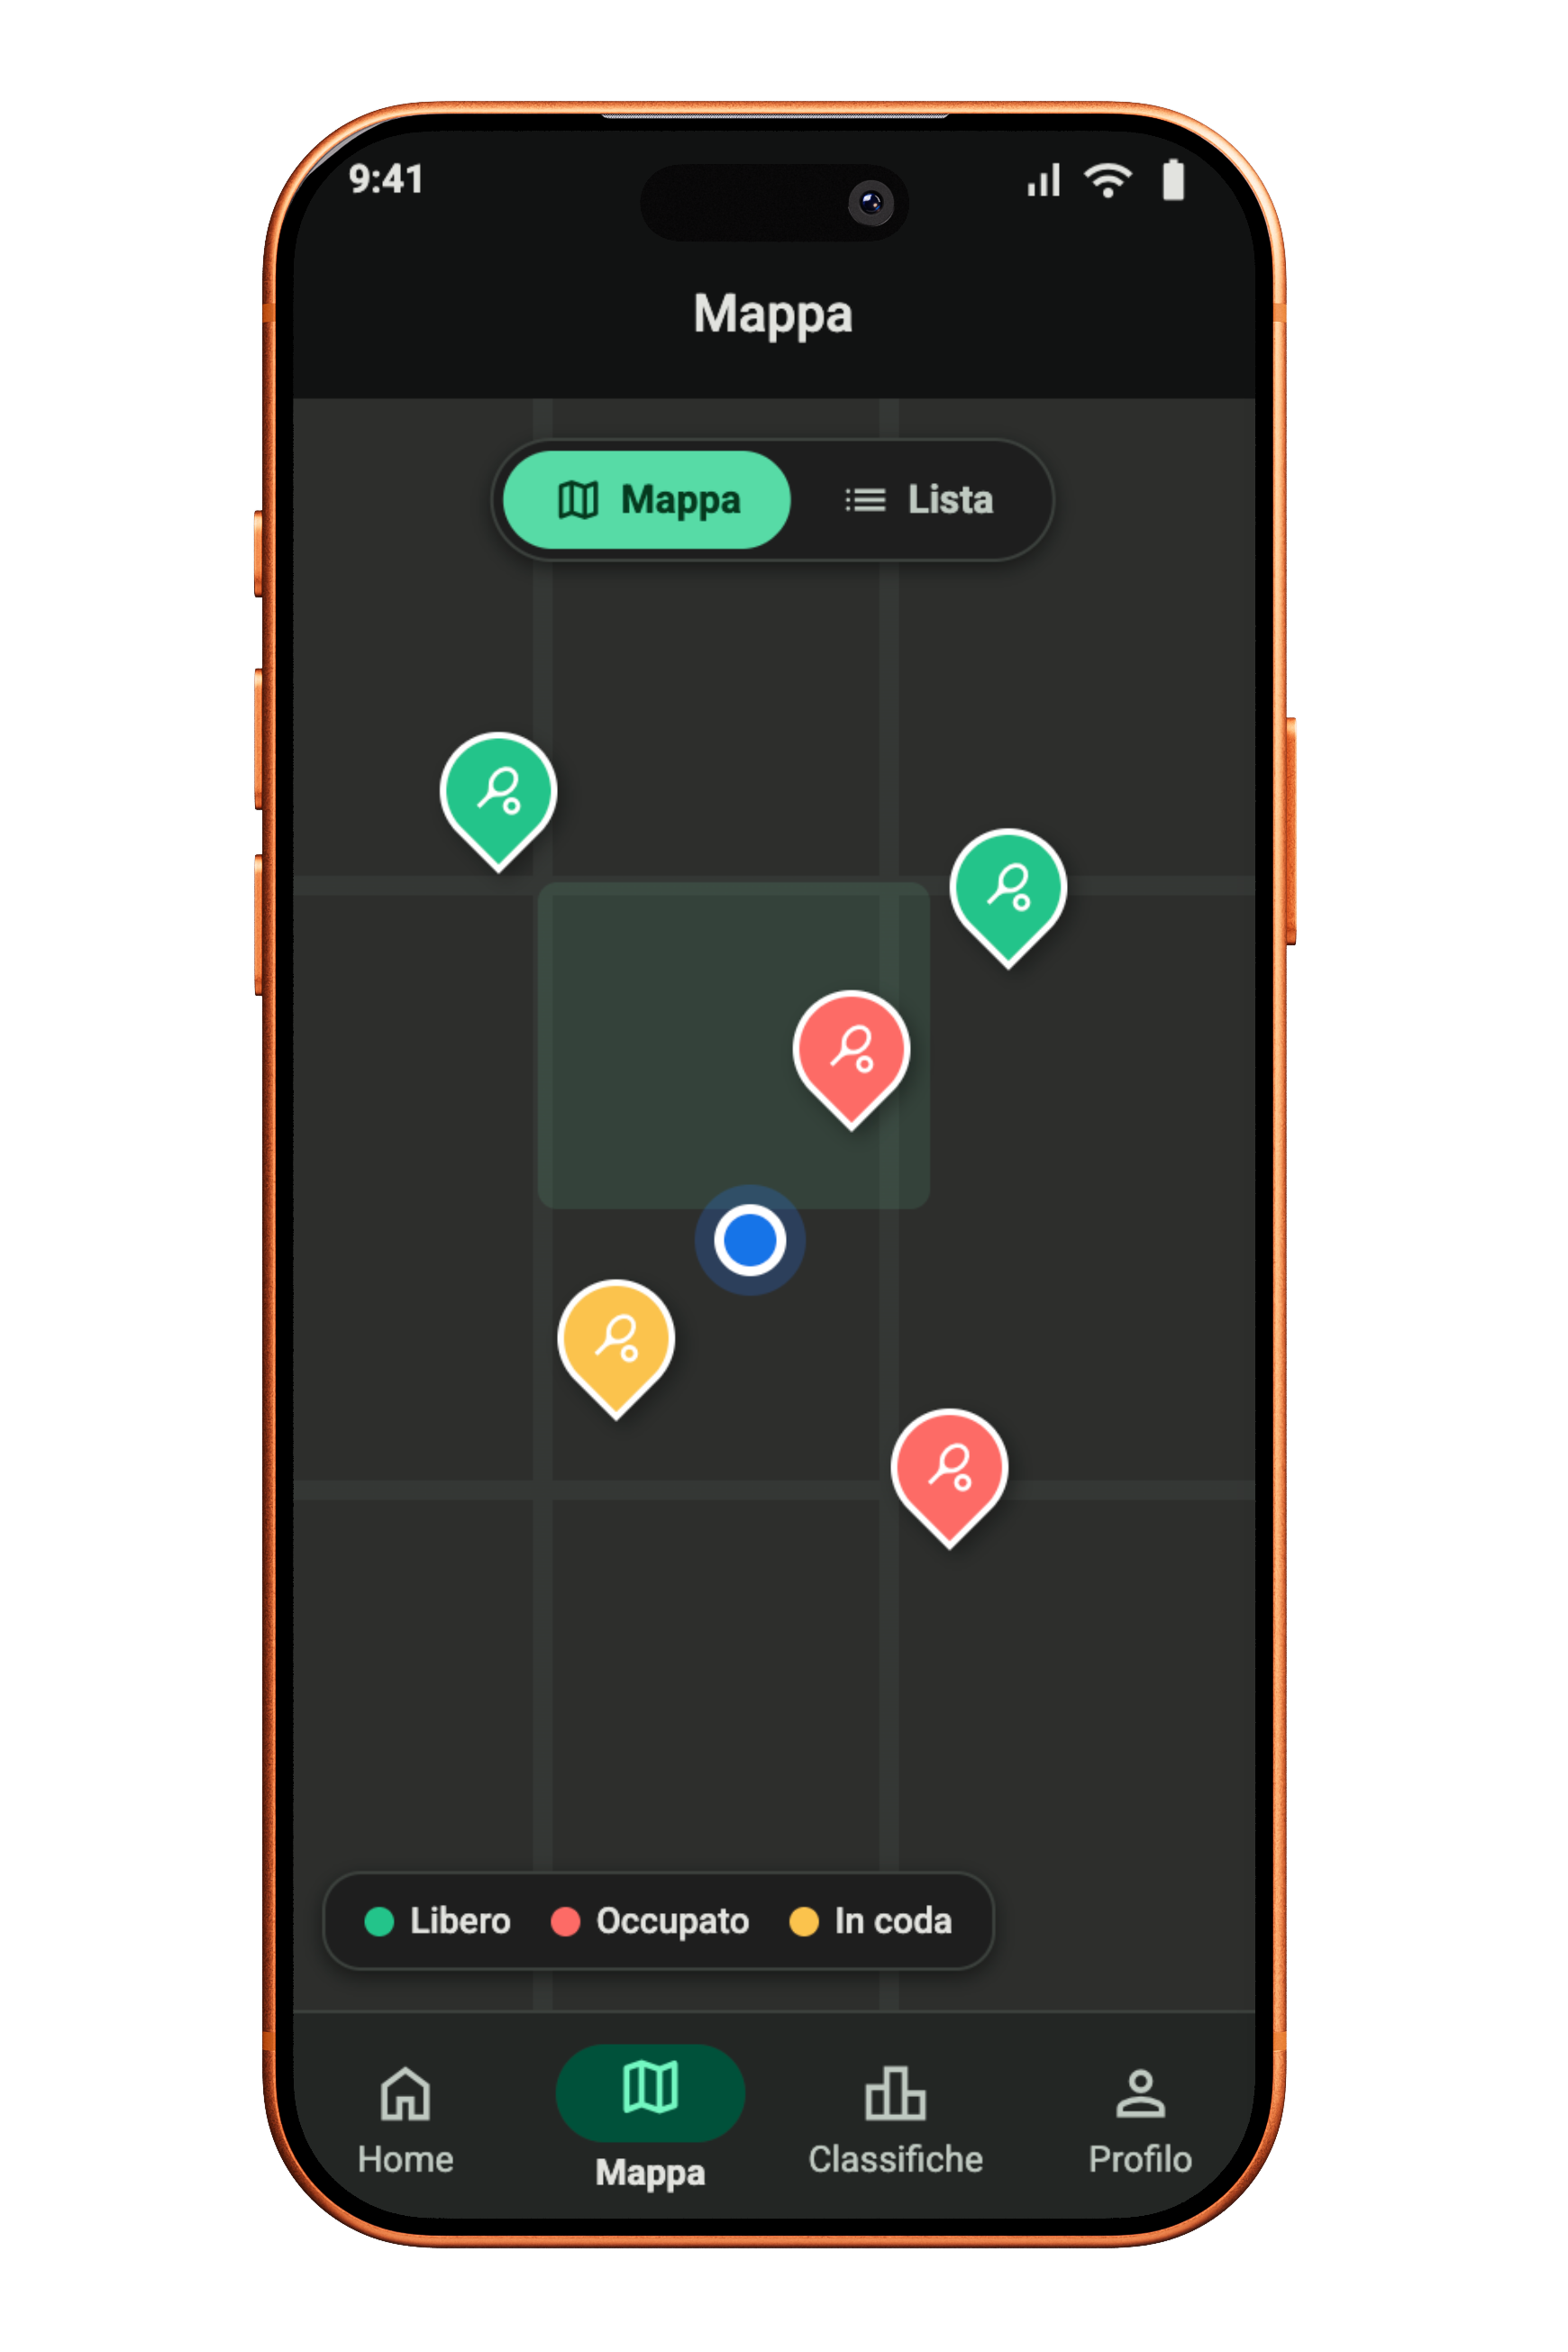
\includegraphics[width=0.25\linewidth]{mockups/map_it_dark}}\hfill
    \subfloat[List view]{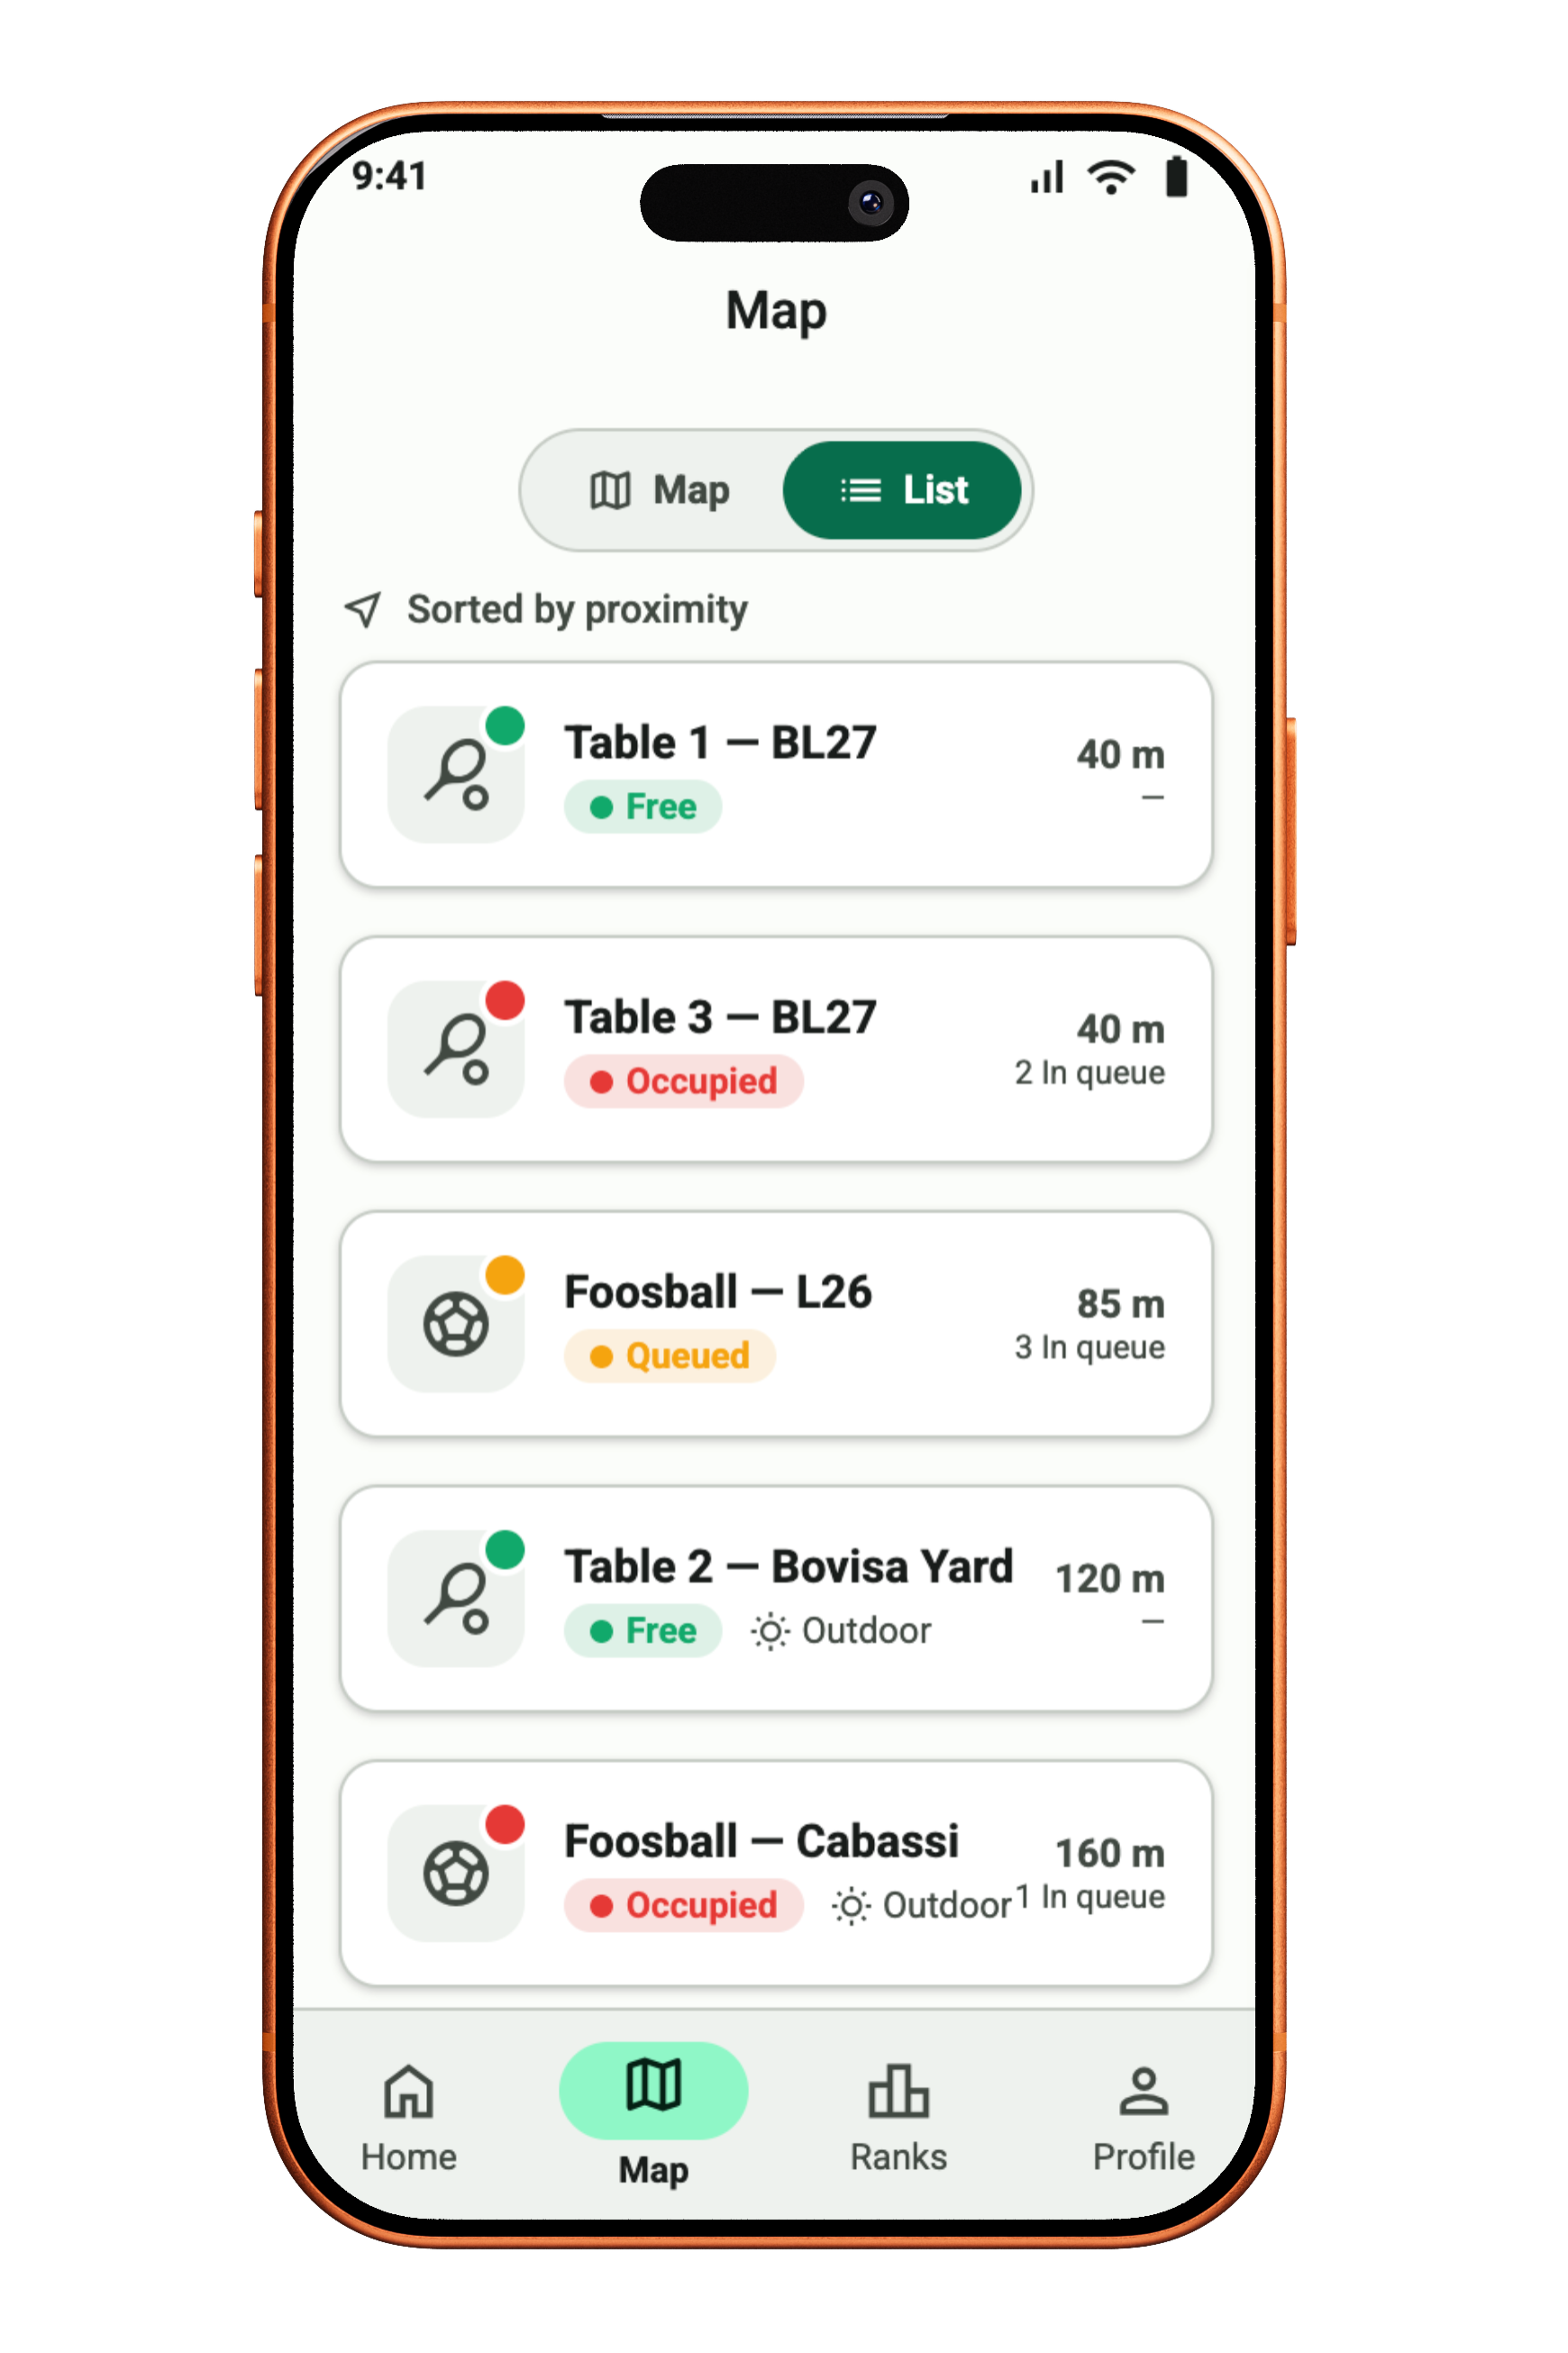
\includegraphics[width=0.25\linewidth]{mockups/list_en_light}}\hfill
    \subfloat[Facility detail]{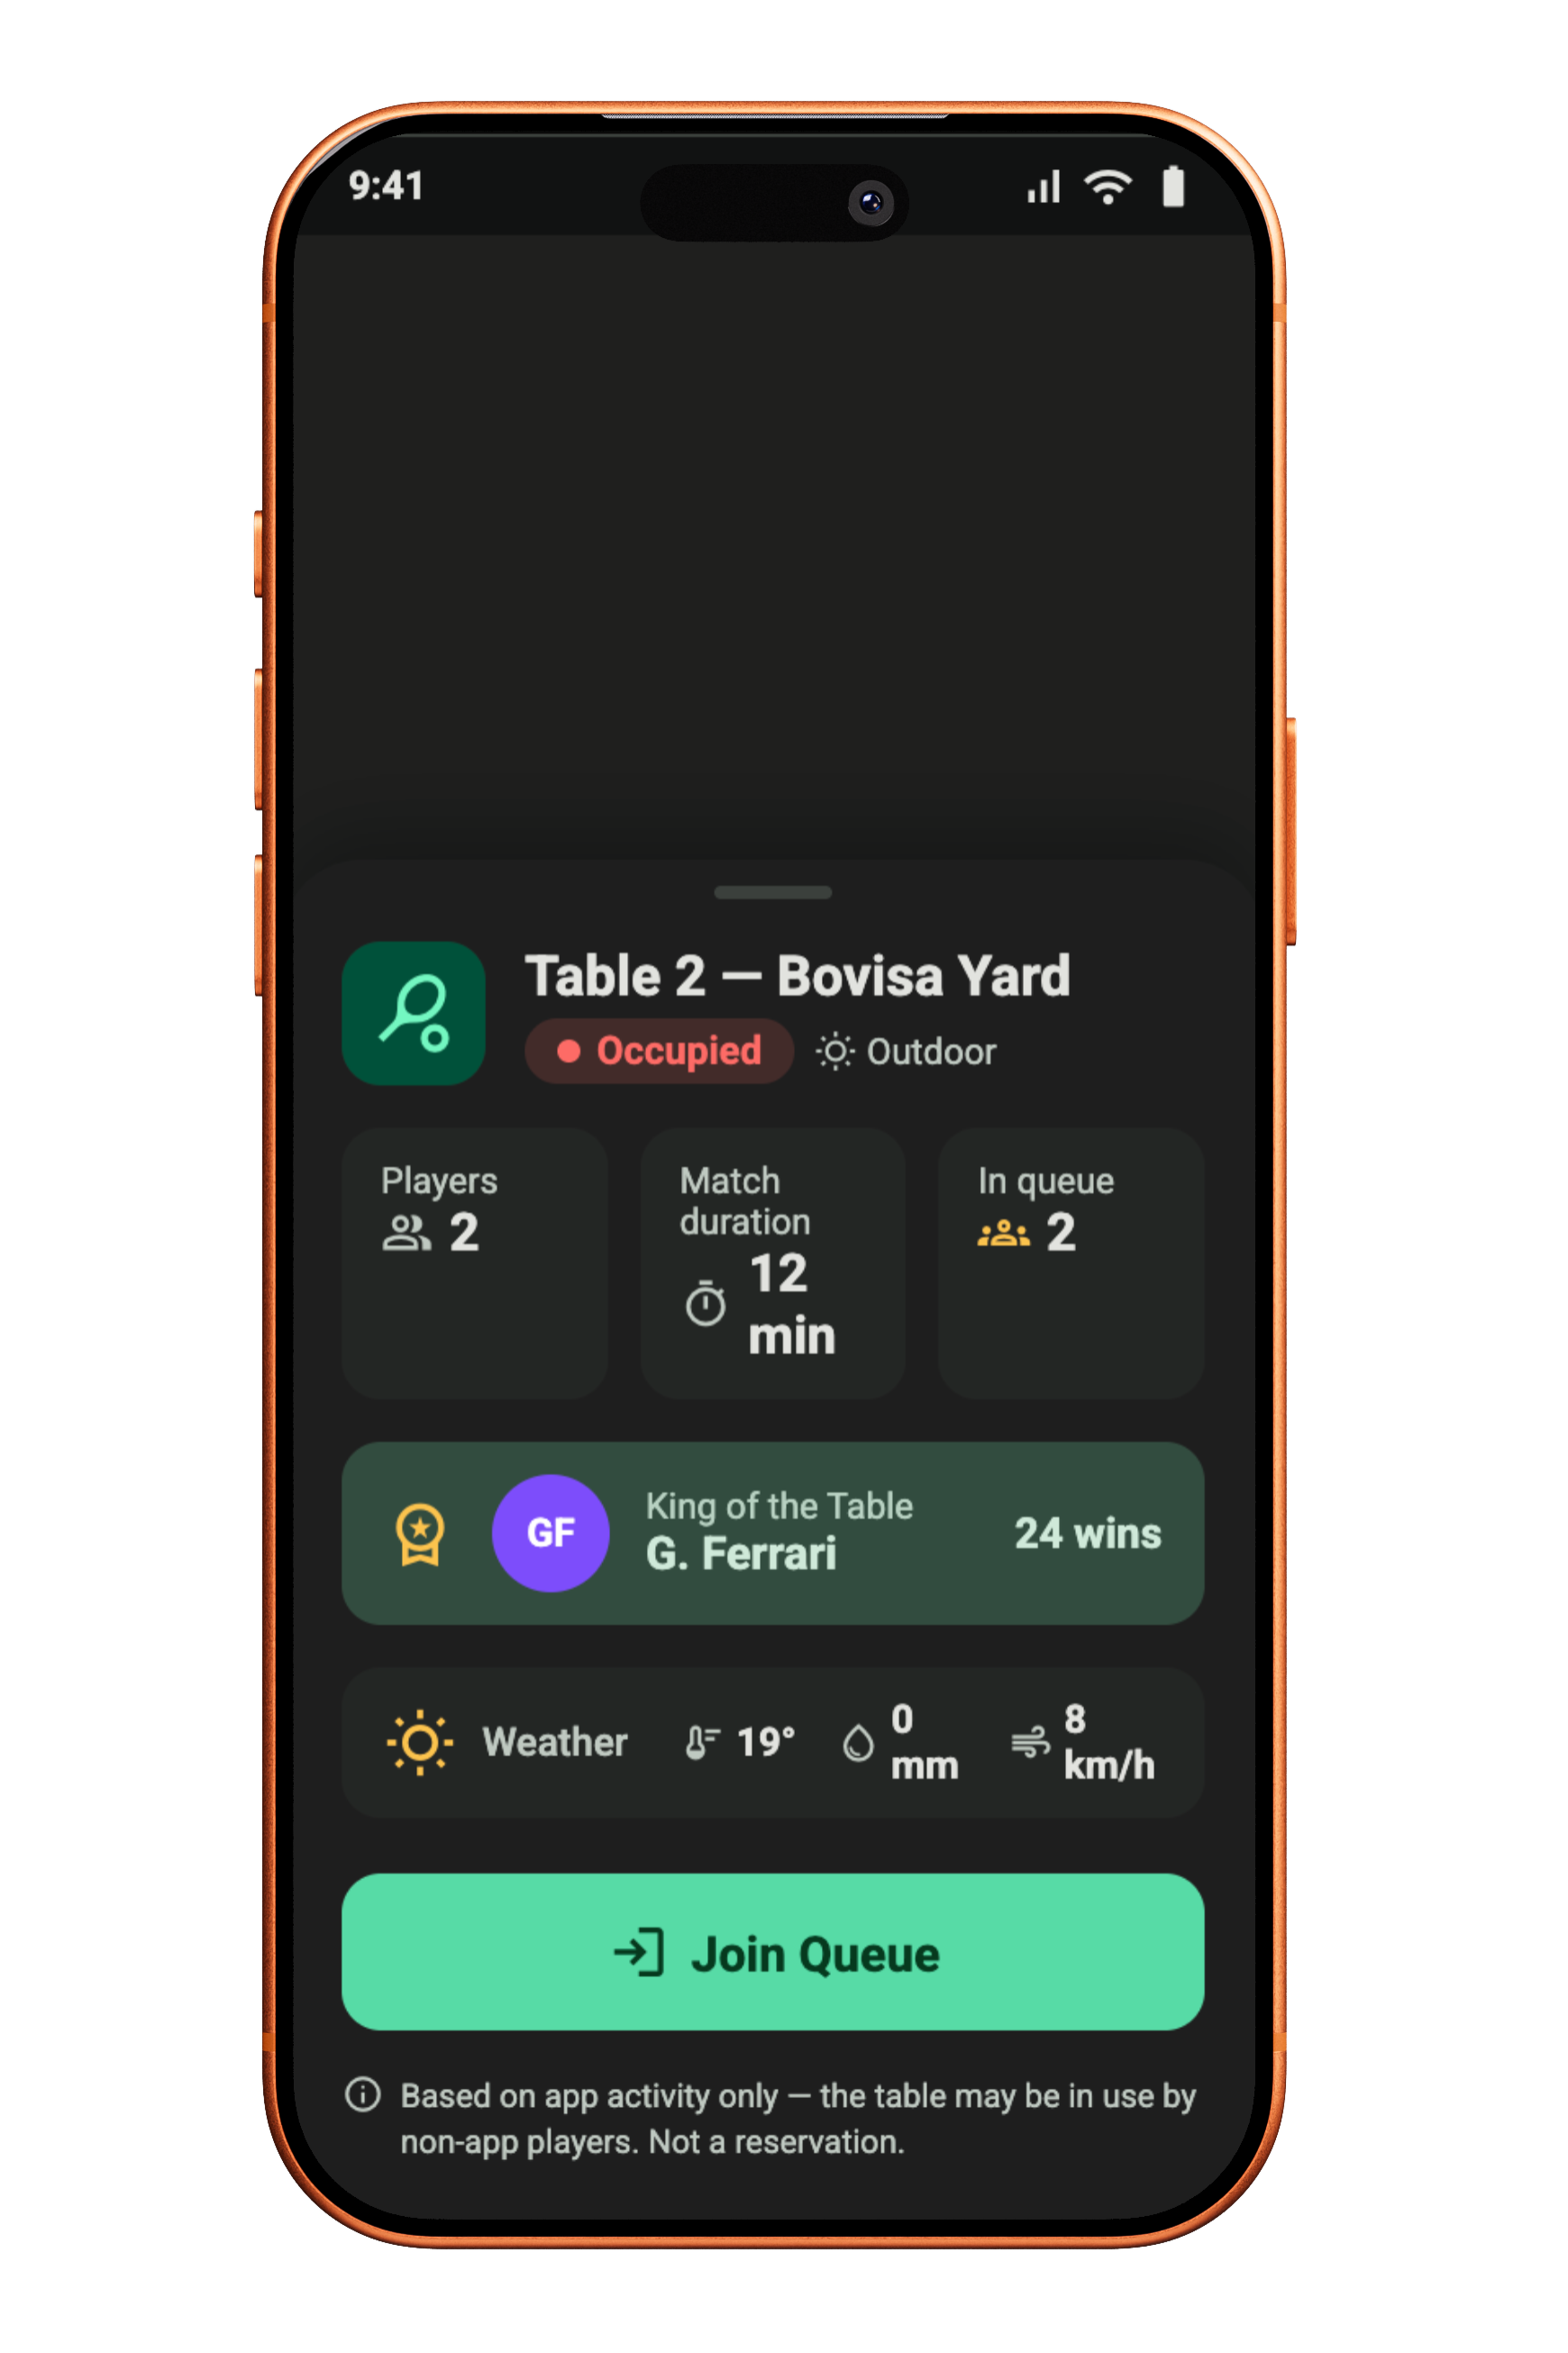
\includegraphics[width=0.25\linewidth]{mockups/facility_en_dark}}
    \caption{Home dashboard, facility map, proximity list, and detail card (with the availability disclaimer footer).}
    \label{fig:map_screens}
\end{figure}

\begin{figure}[H]
    \centering
    \subfloat[QR scan]{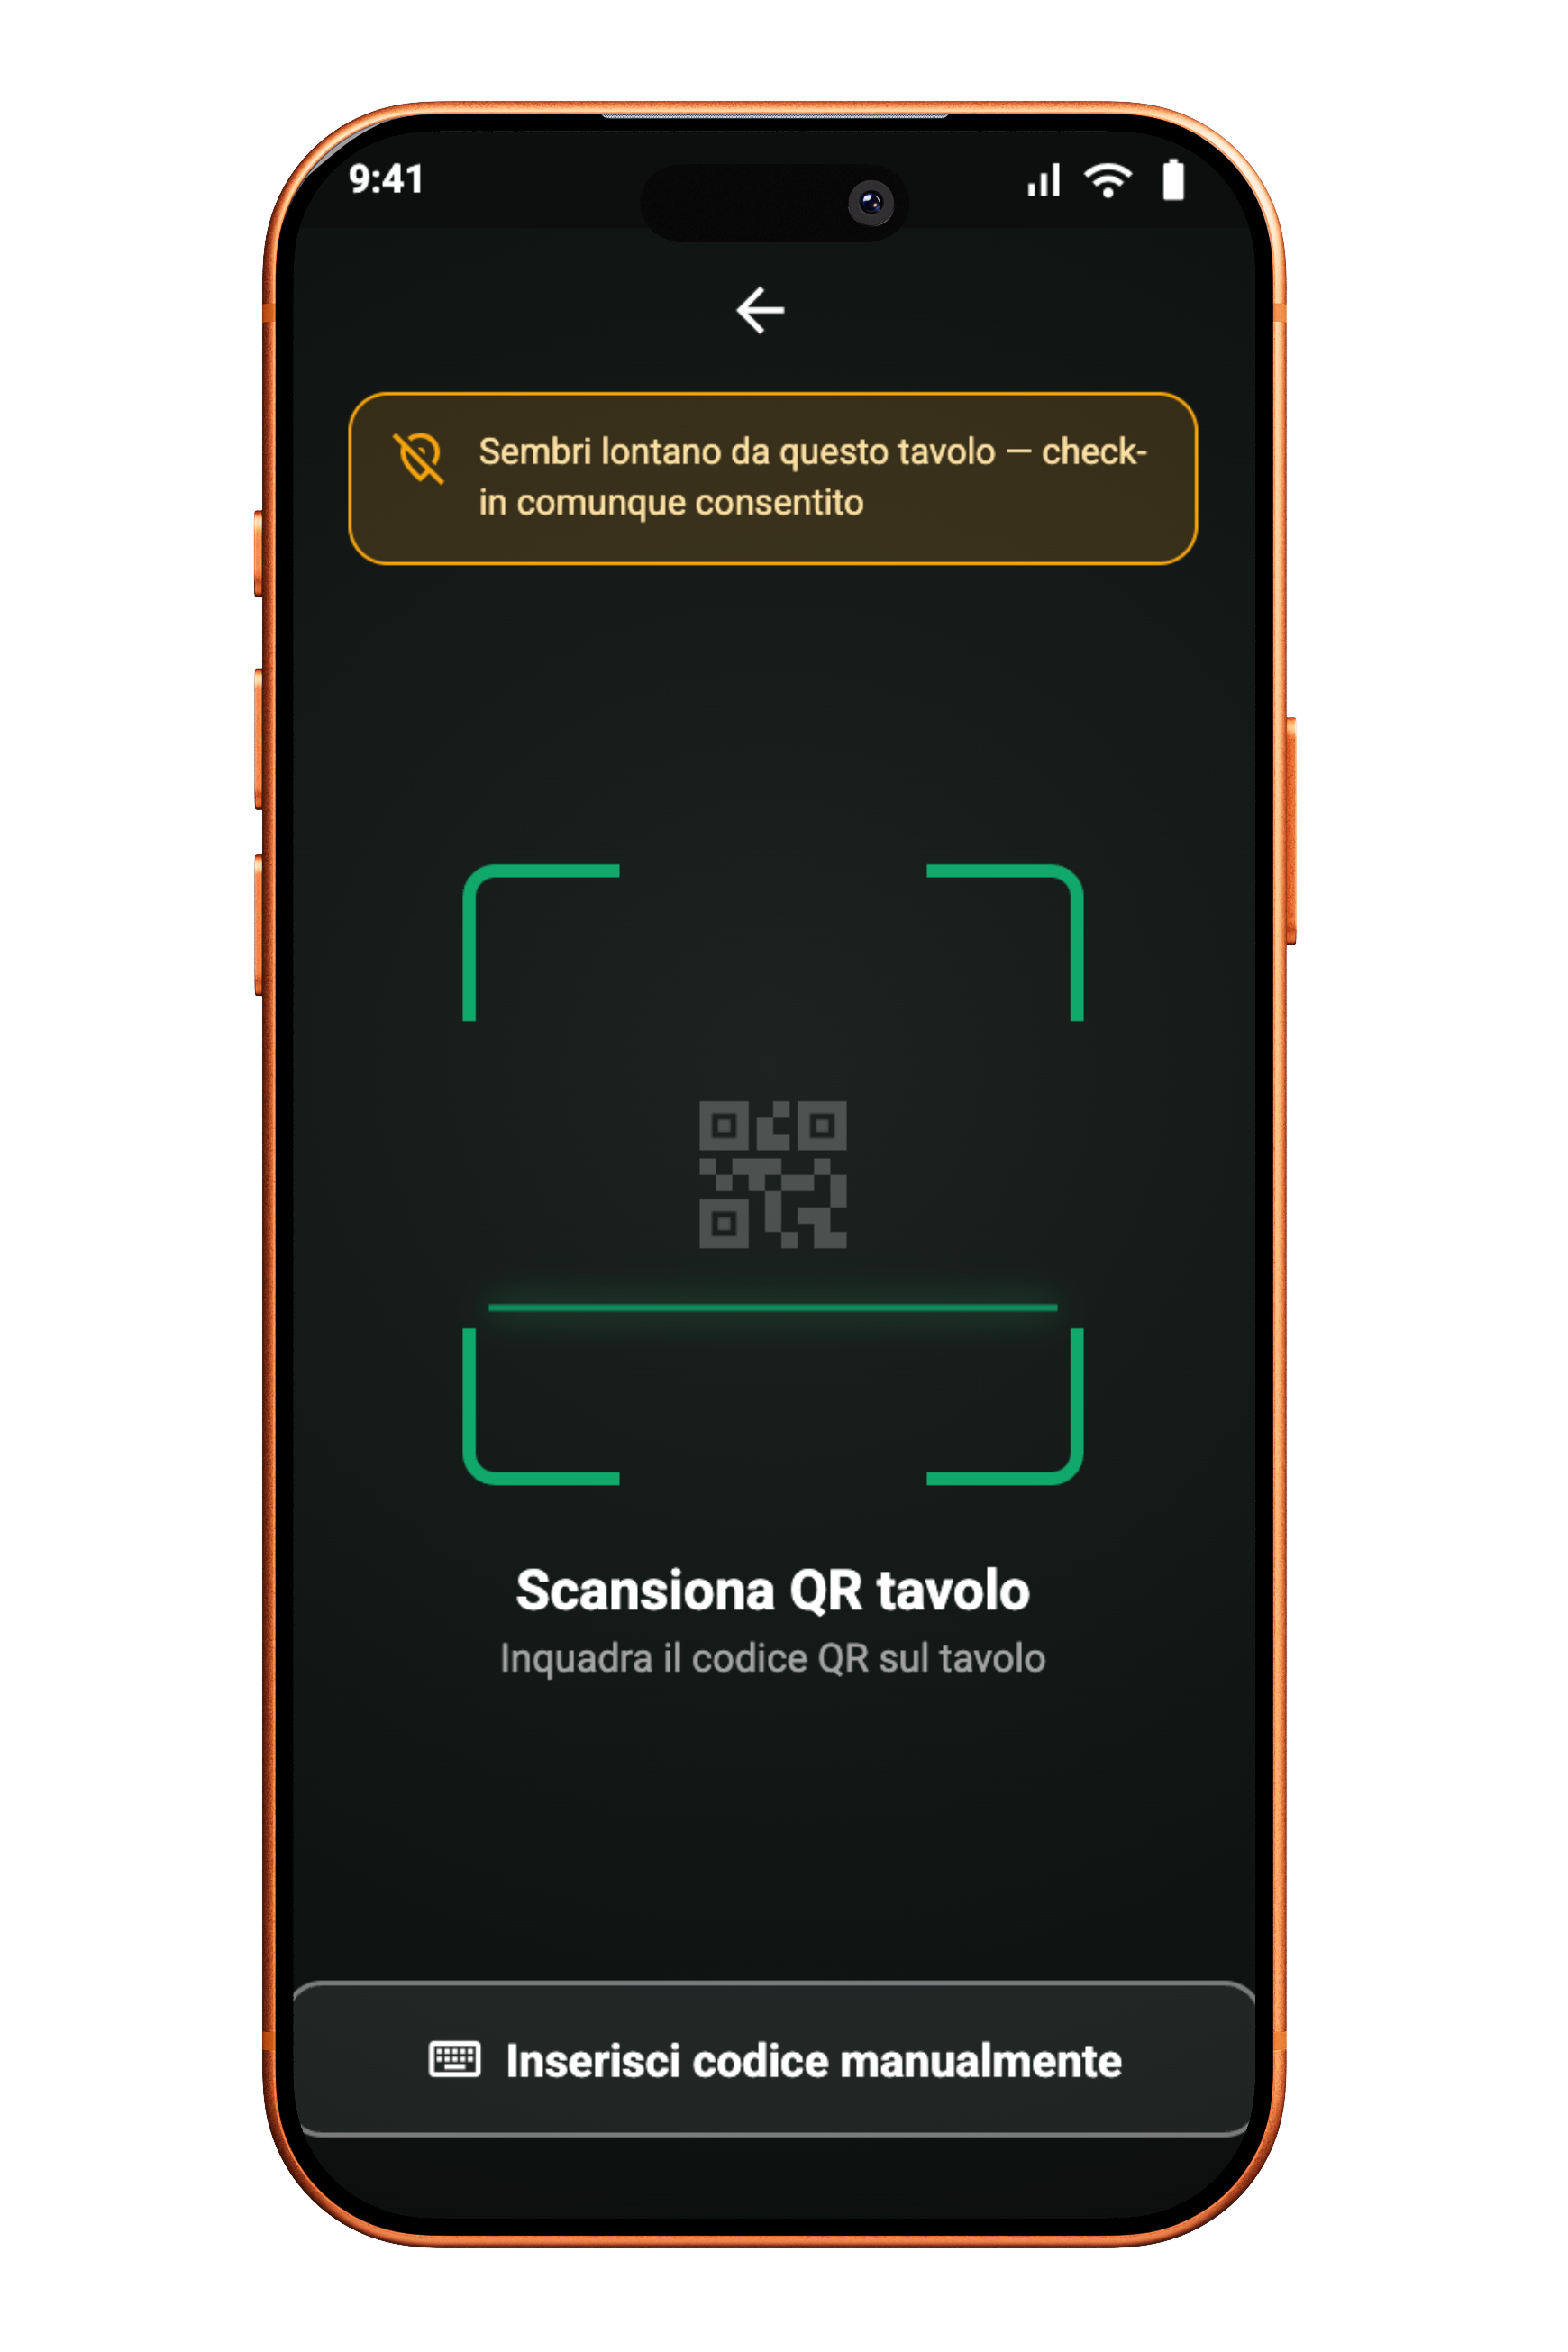
\includegraphics[width=0.2\linewidth]{mockups/scan_it_light}}\hfill
    \subfloat[Active match]{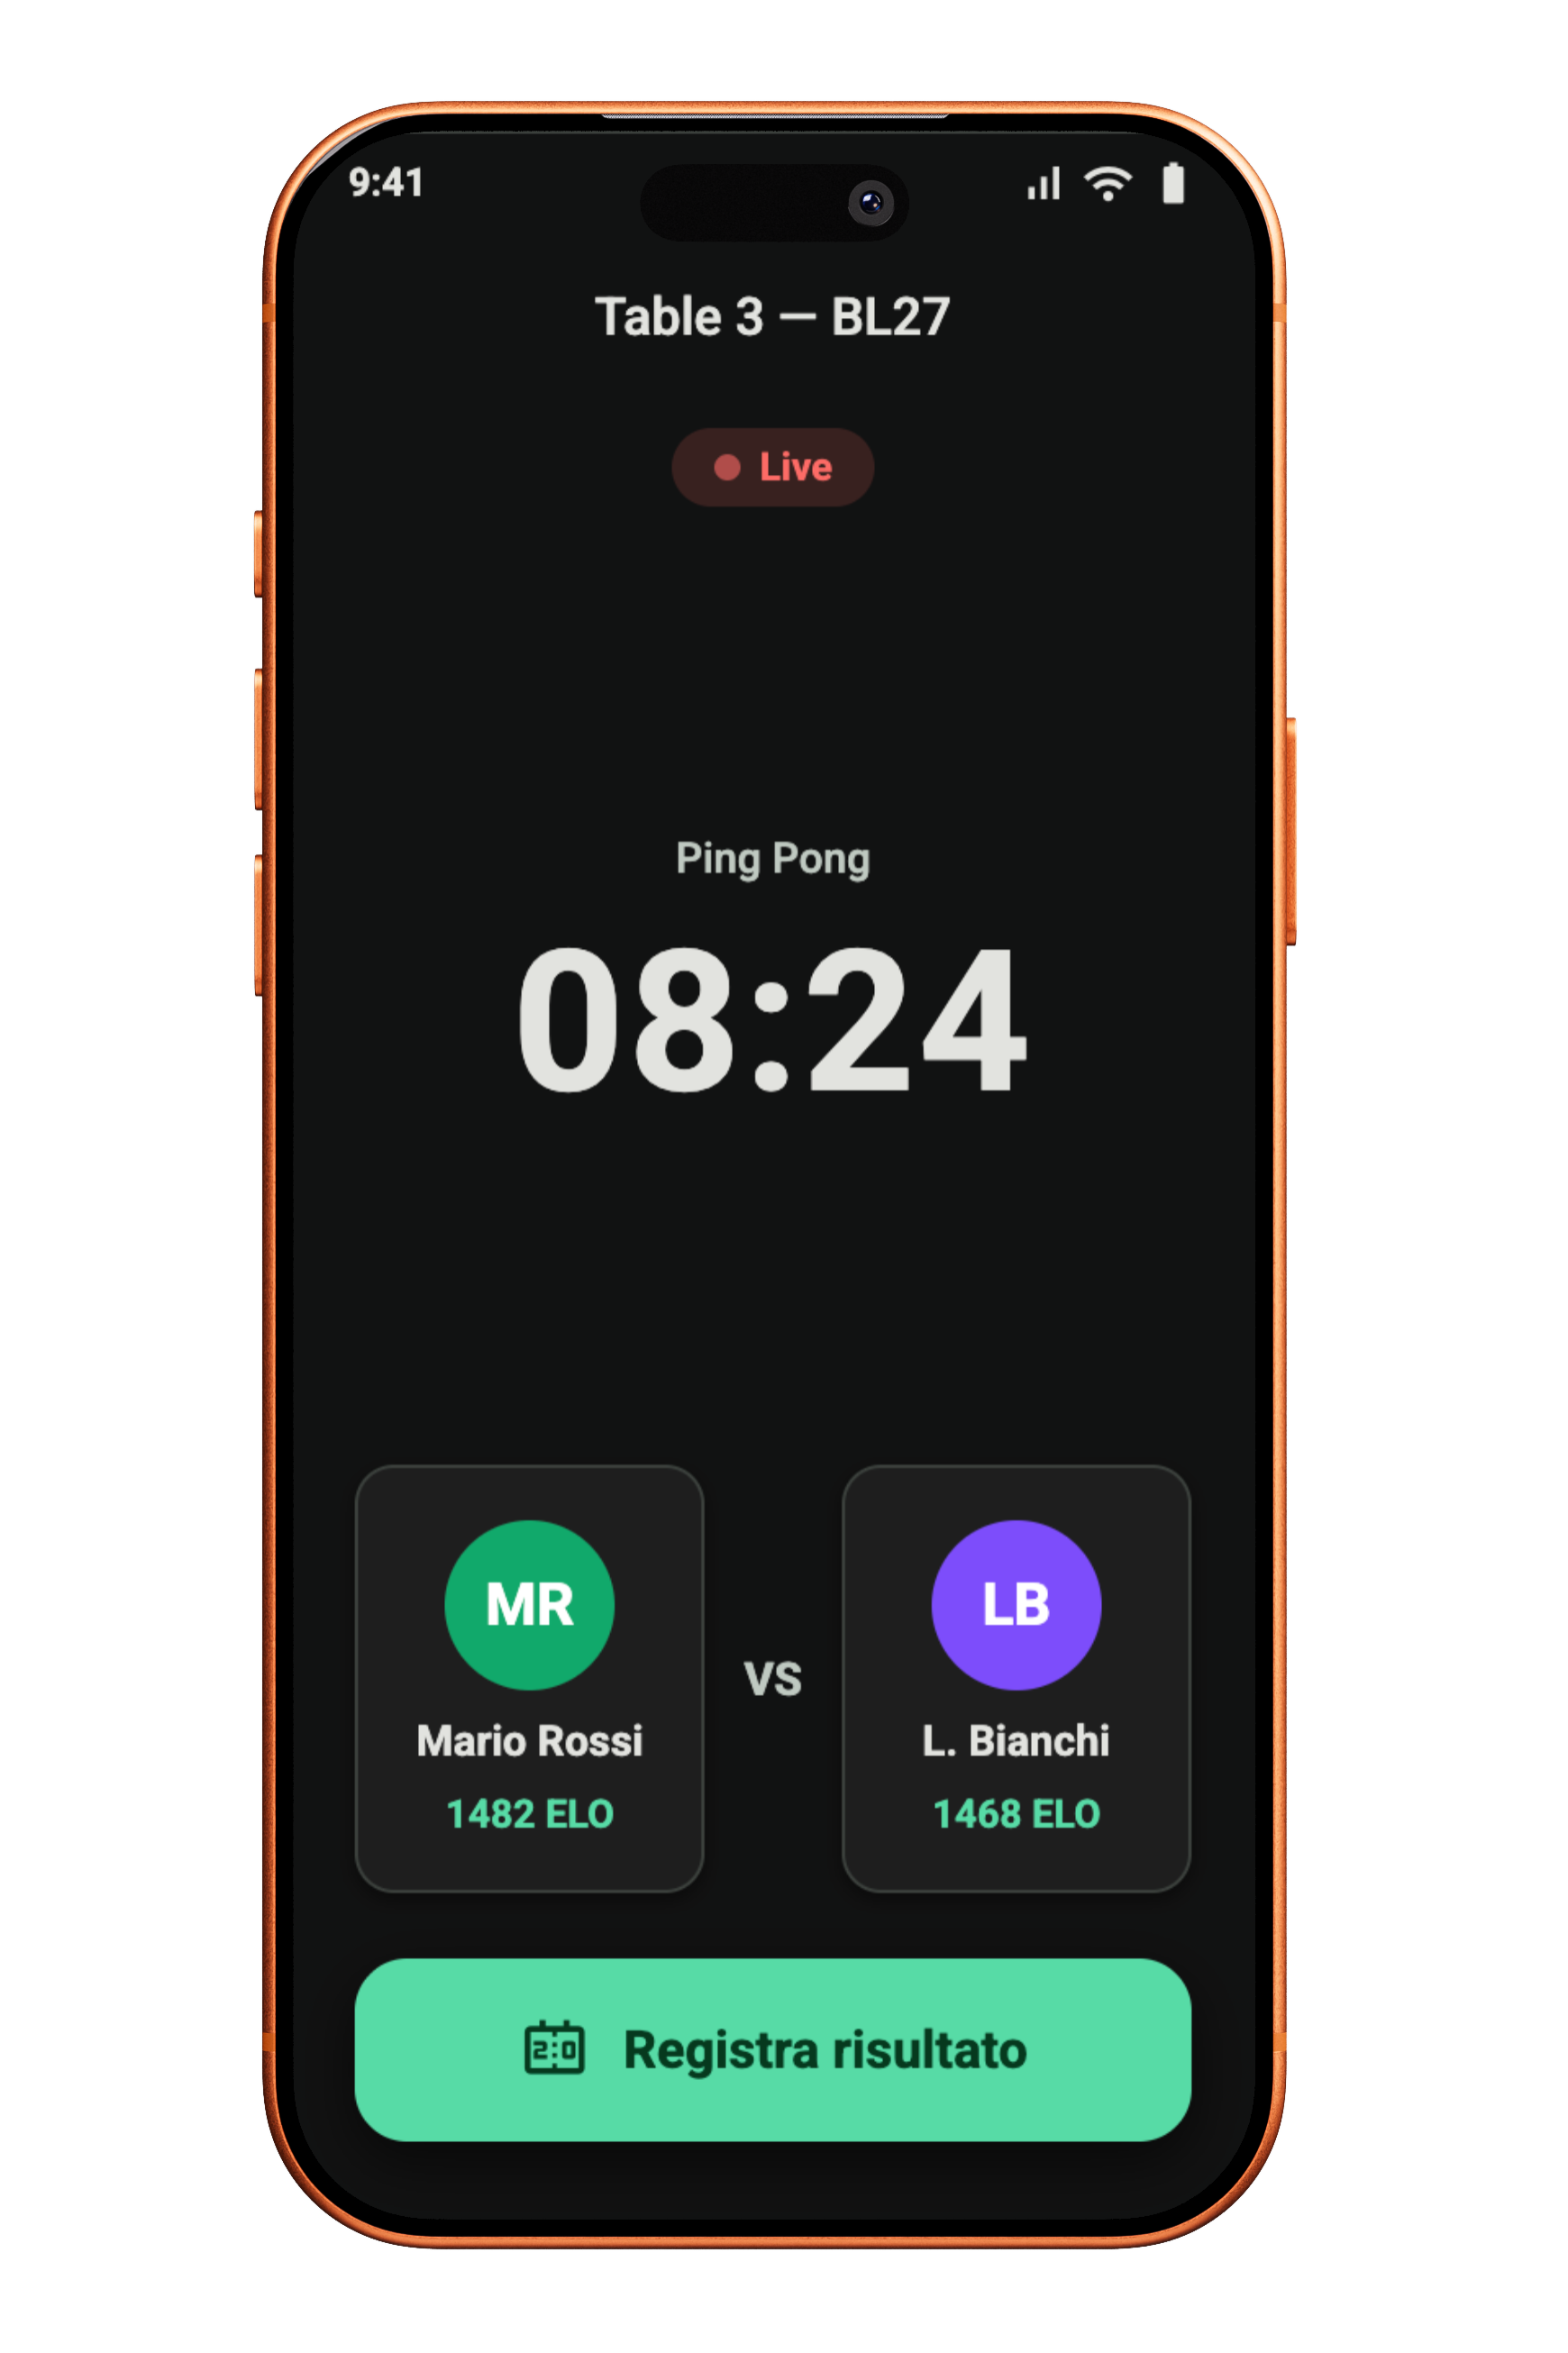
\includegraphics[width=0.2\linewidth]{mockups/active_it_dark}}\hfill
    \subfloat[Result entry]{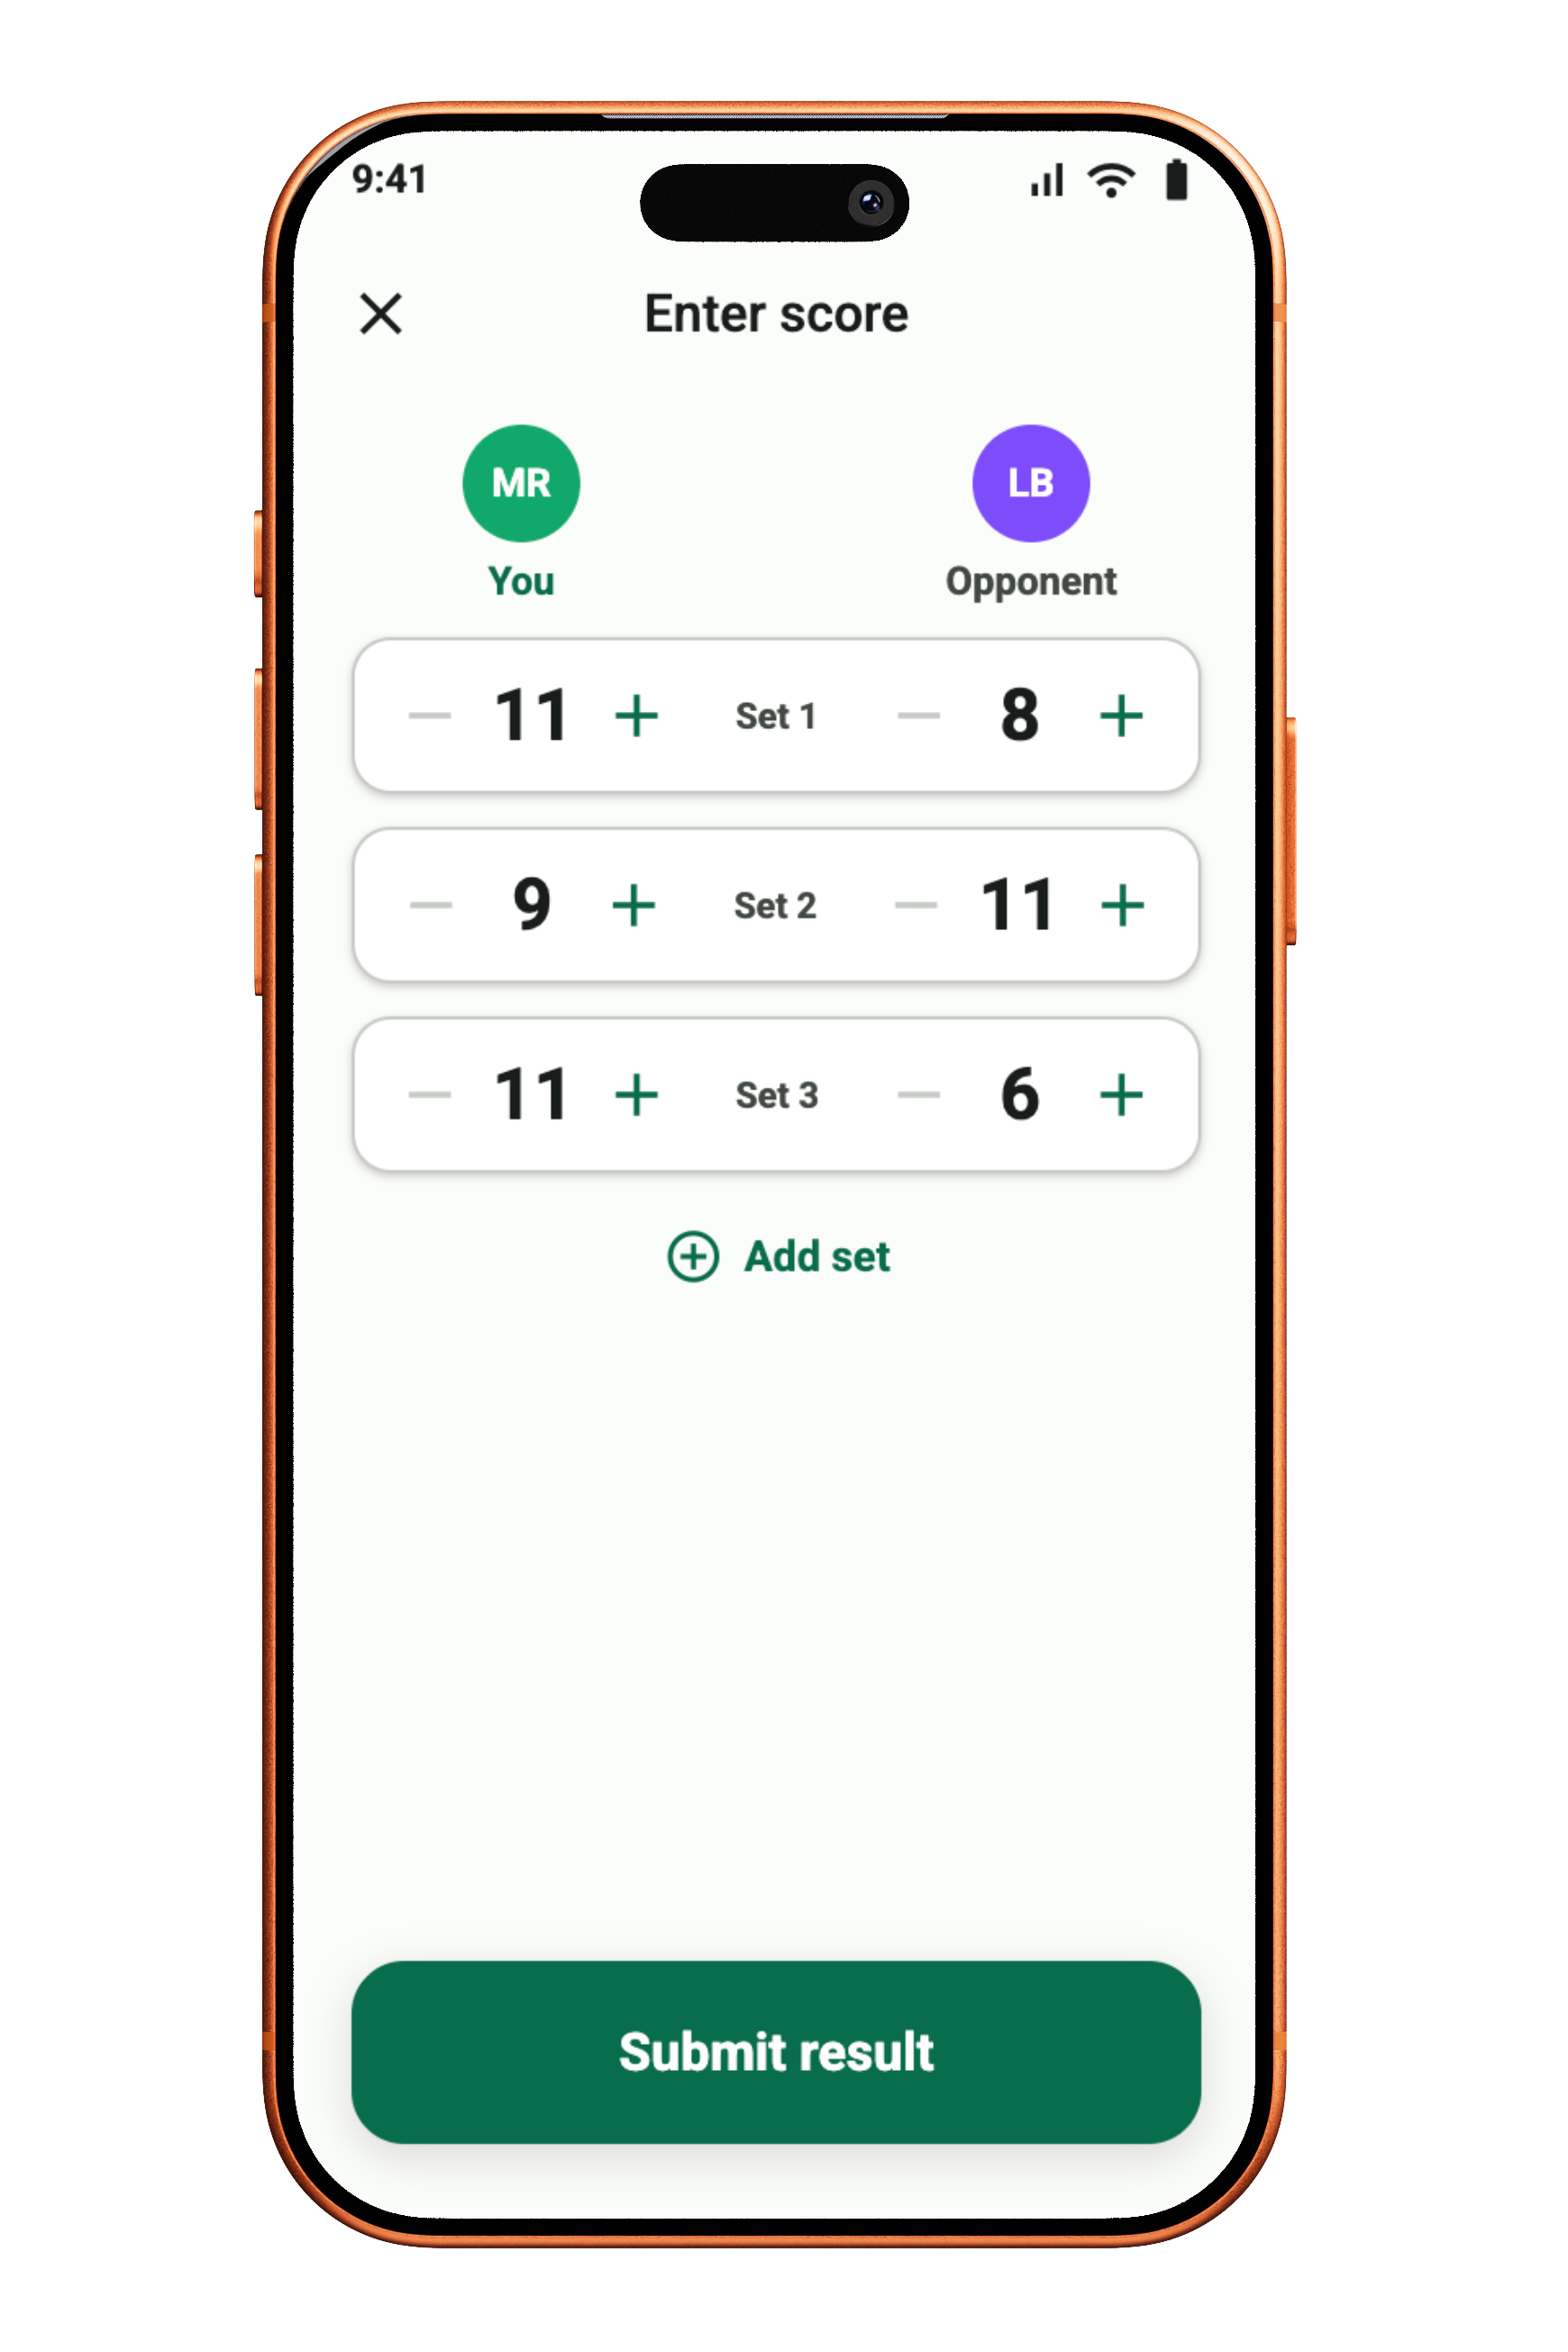
\includegraphics[width=0.2\linewidth]{mockups/score_en_light}}\hfill
    \subfloat[Confirmation]{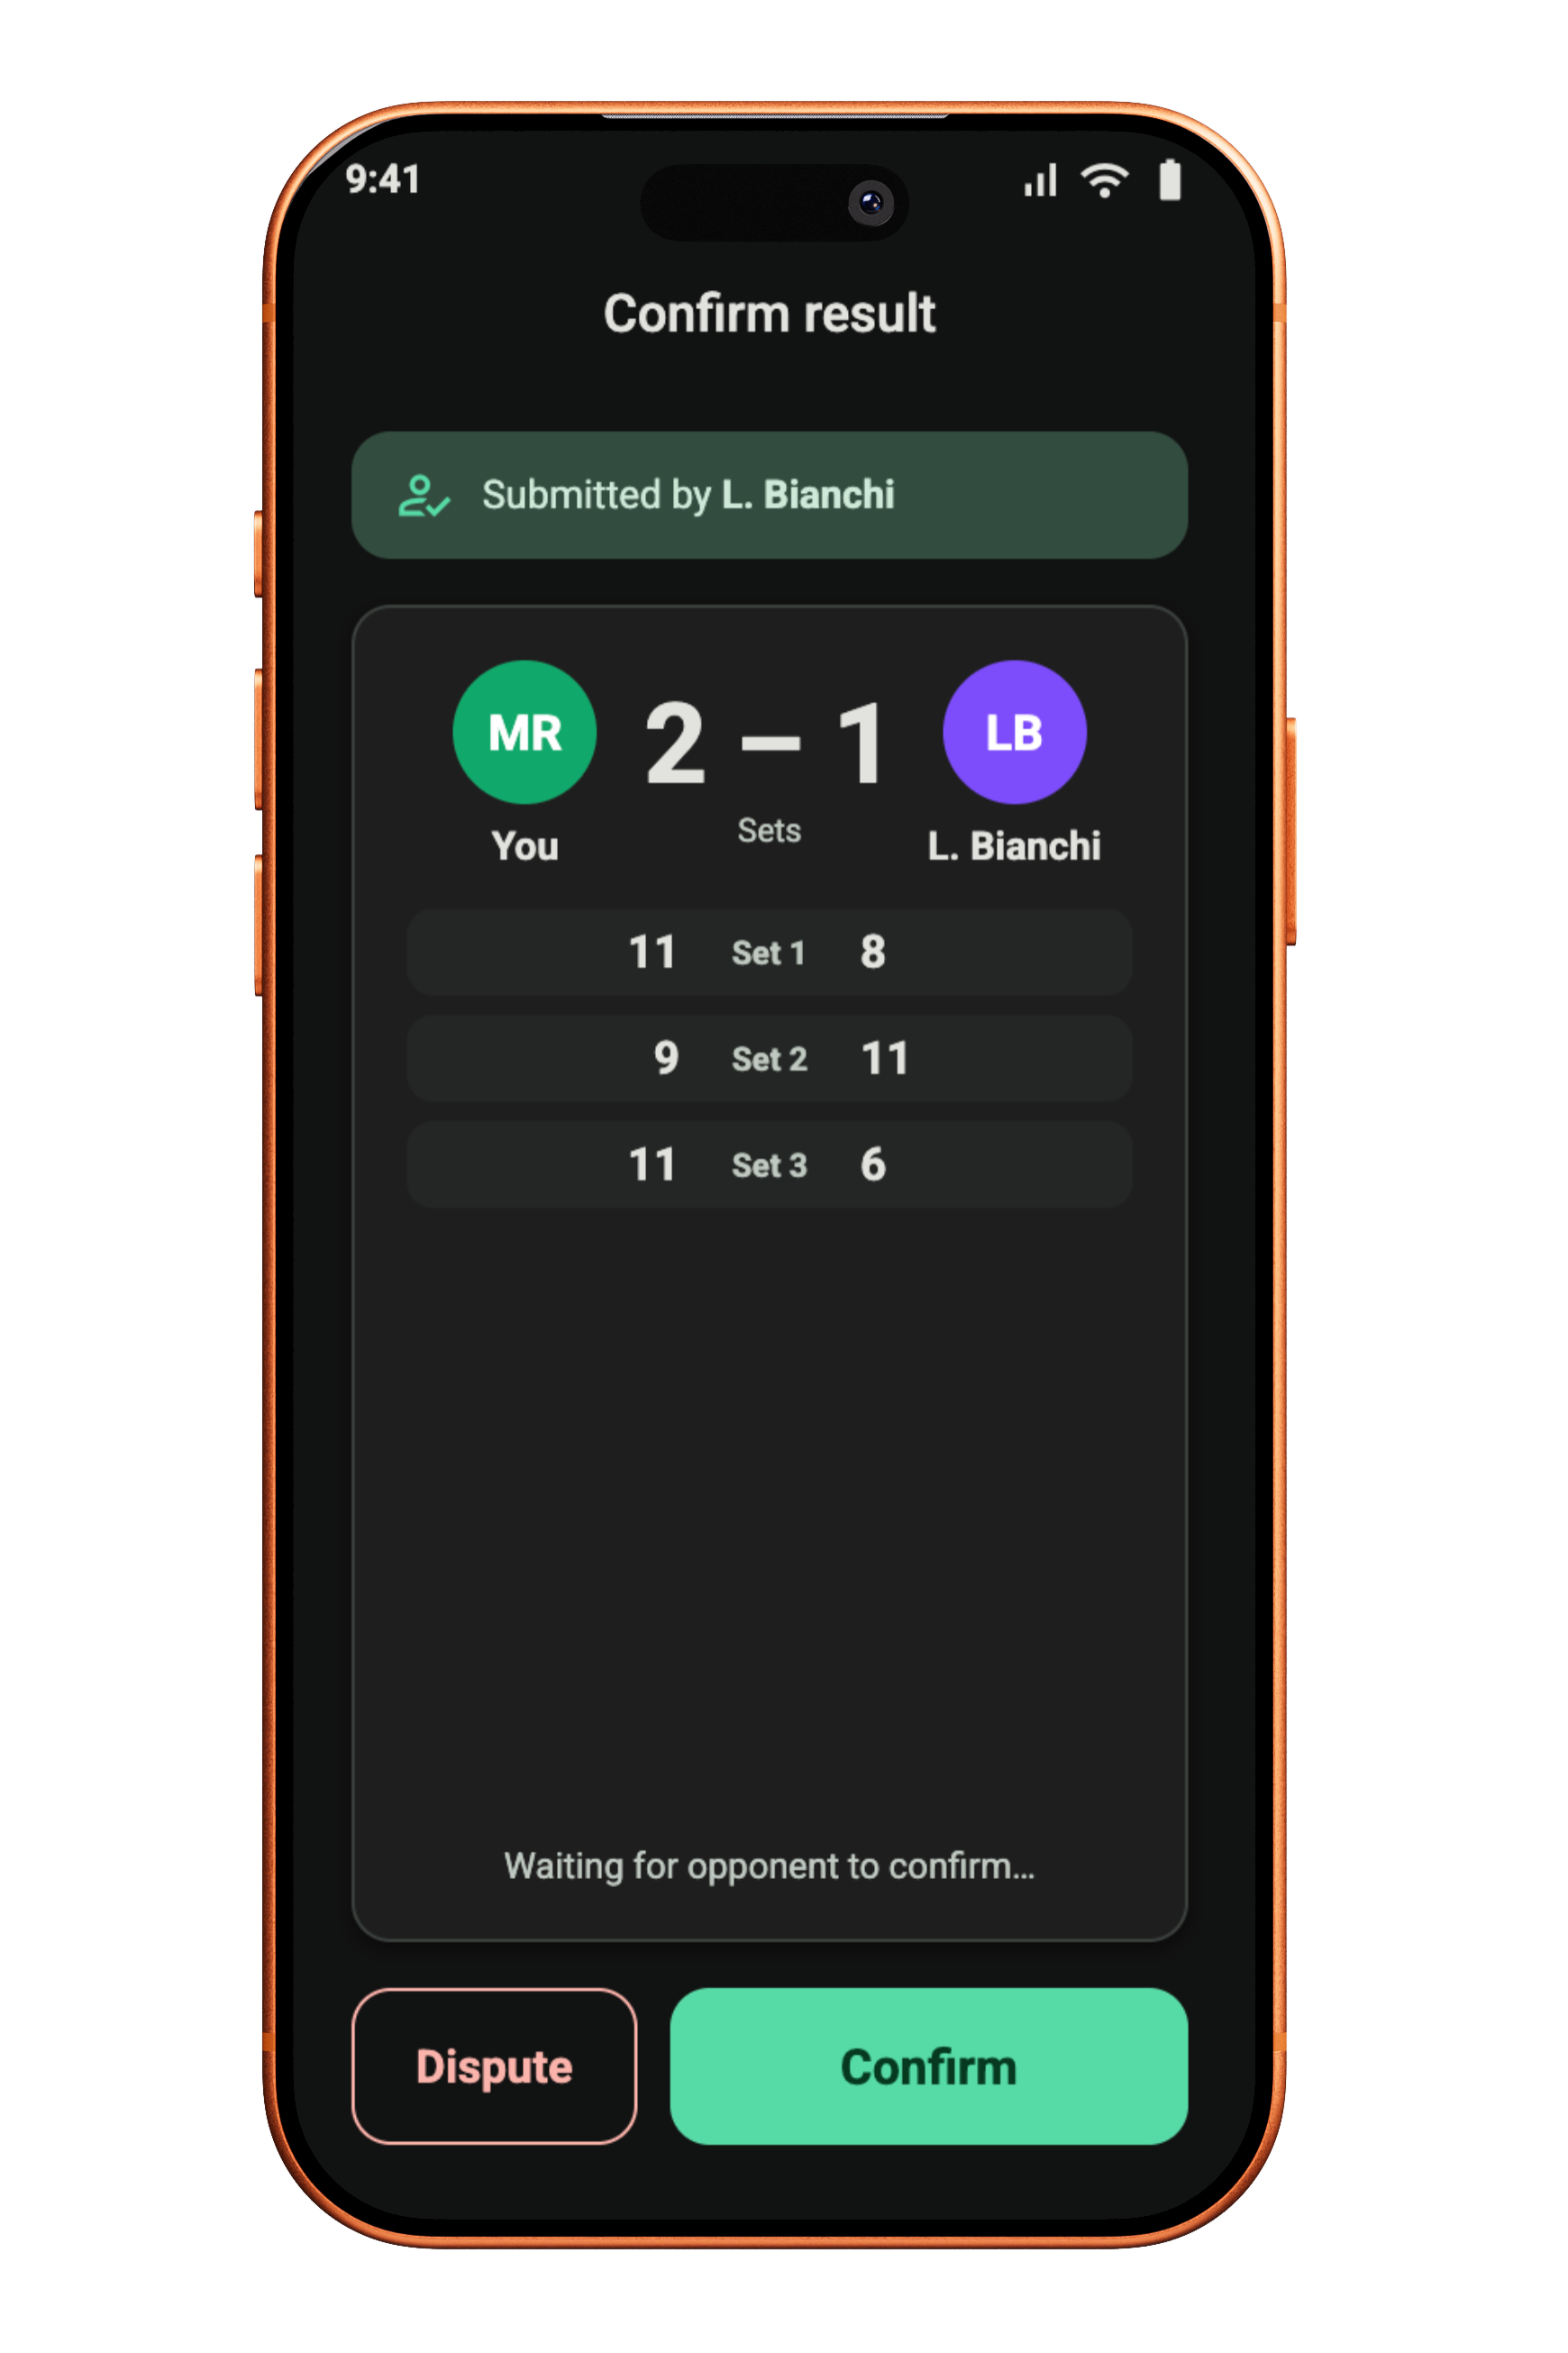
\includegraphics[width=0.2\linewidth]{mockups/confirm_en_dark}}\hfill
    \subfloat[Summary]{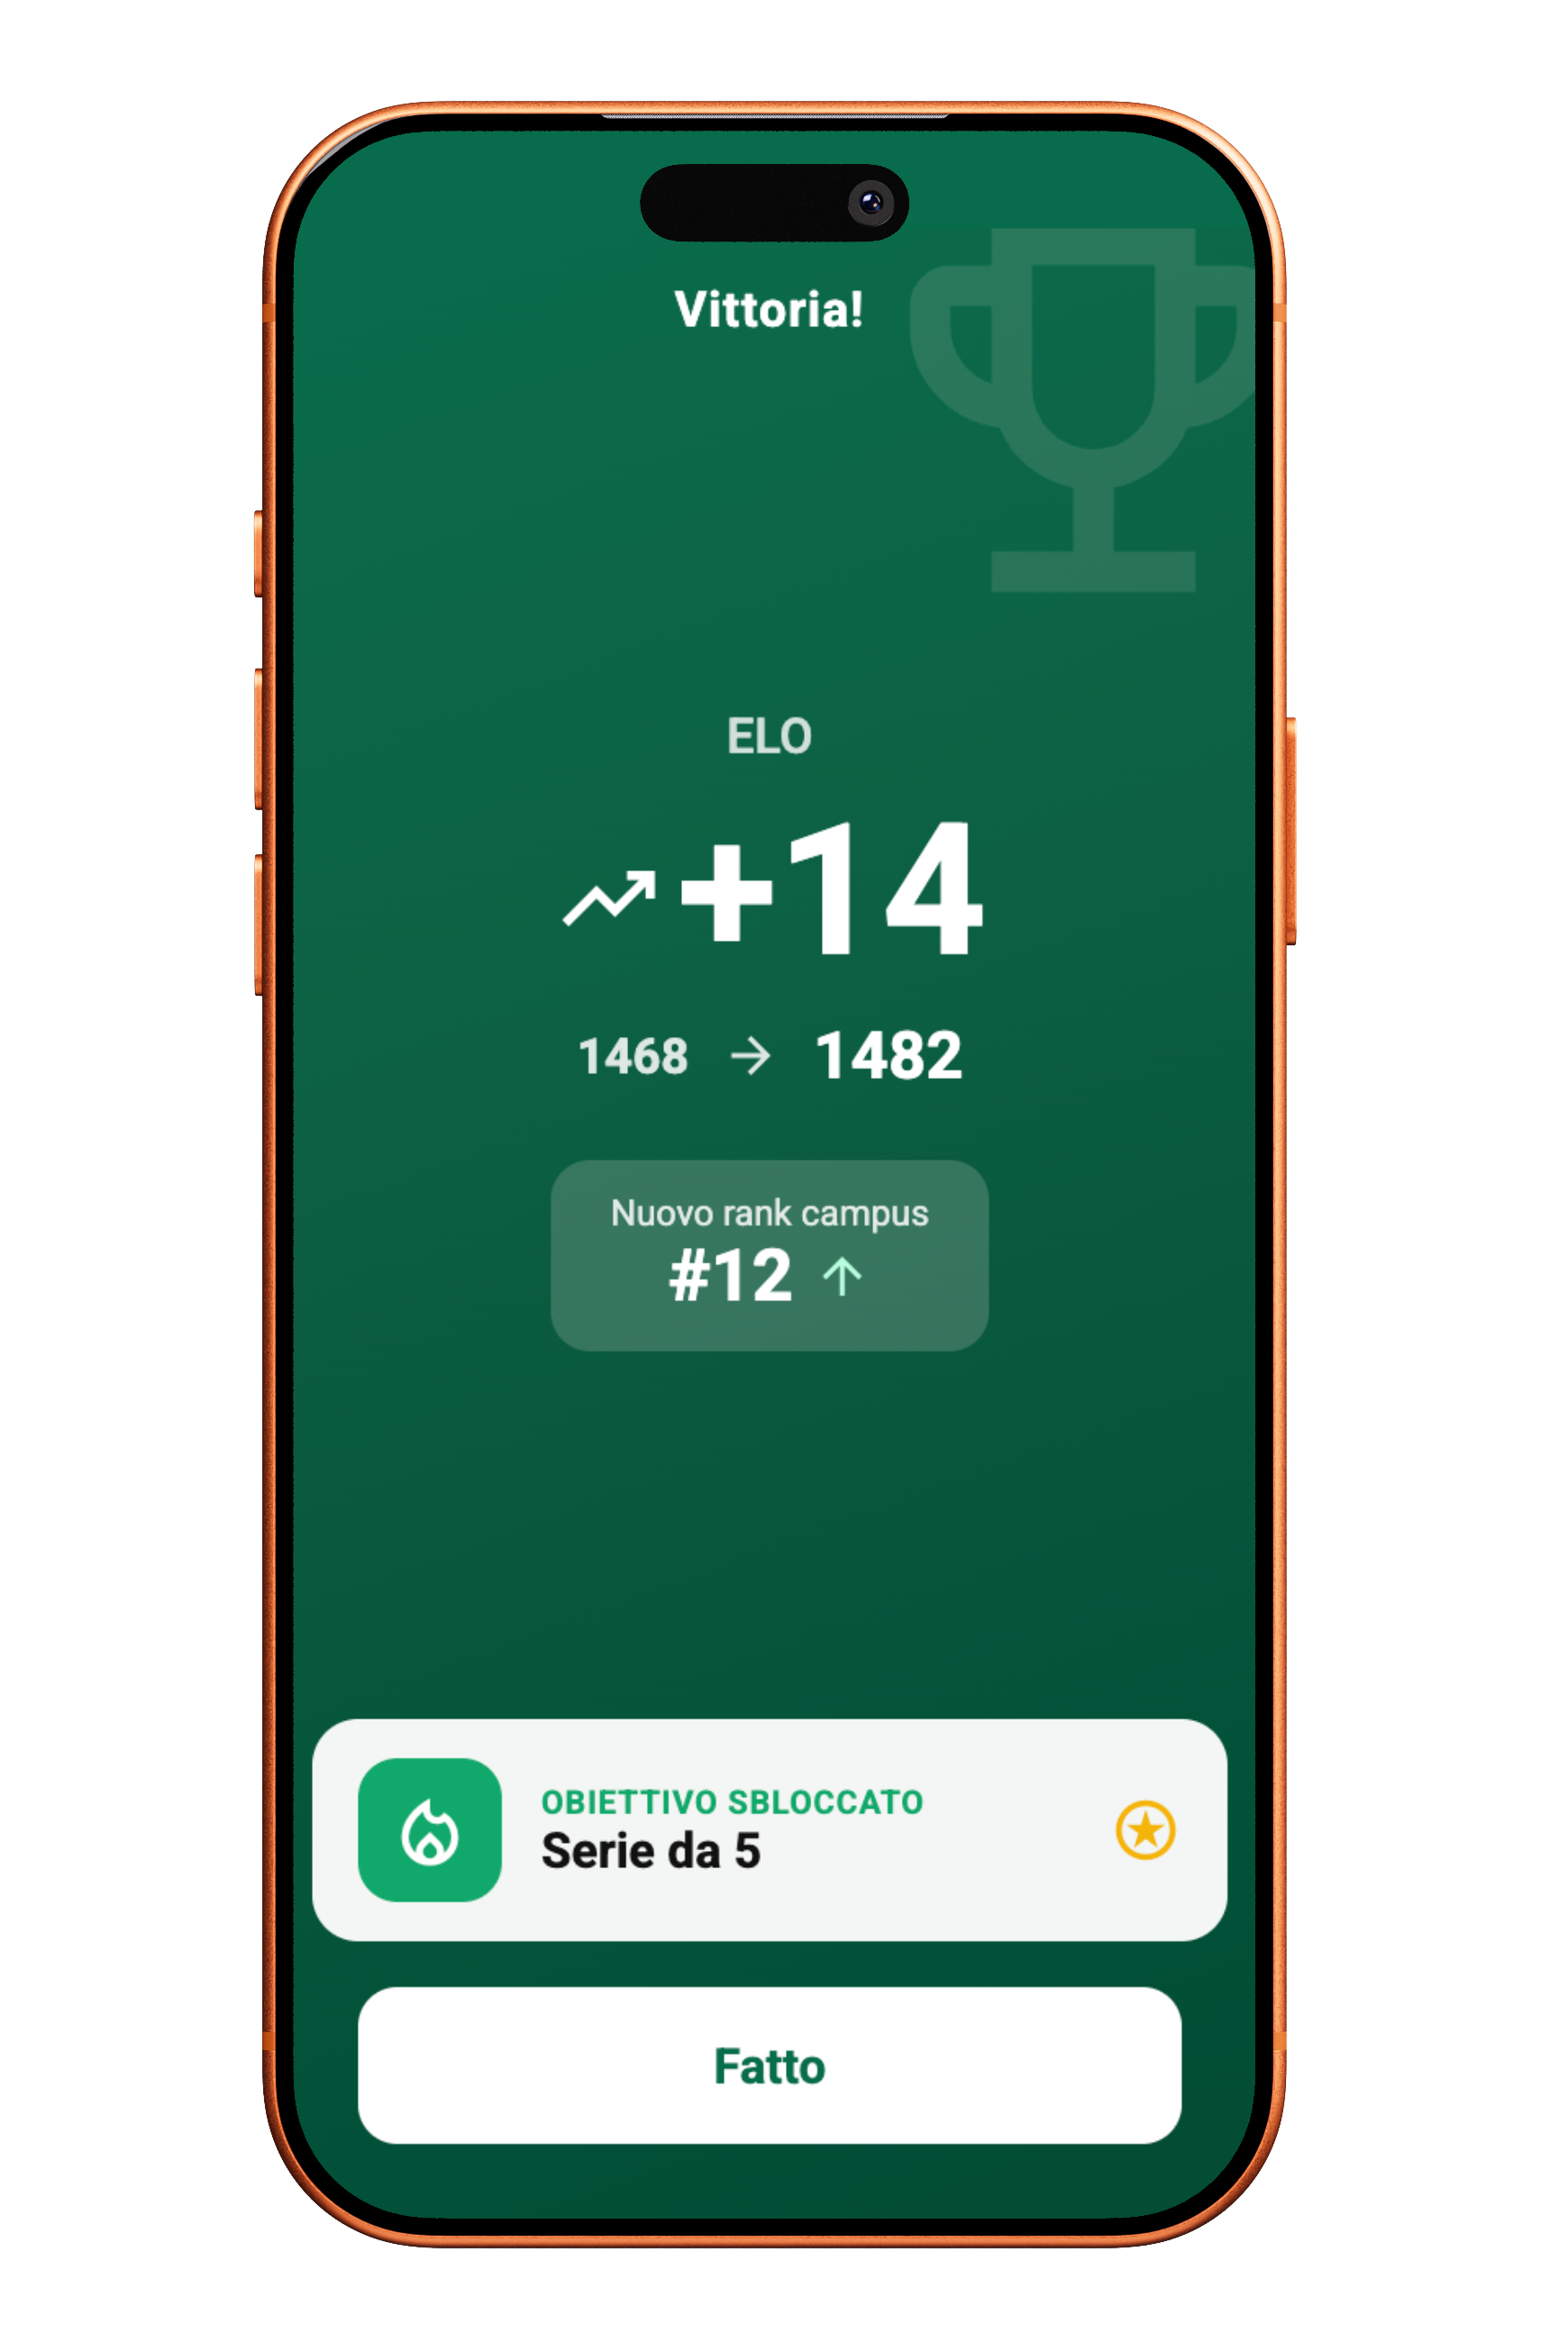
\includegraphics[width=0.2\linewidth]{mockups/result_it_light}}
    \caption{The Proof-of-Play match flow, from QR scan to ELO-delta summary.}
    \label{fig:match_screens}
\end{figure}

\begin{figure}[H]
    \centering
    \subfloat[Leaderboard]{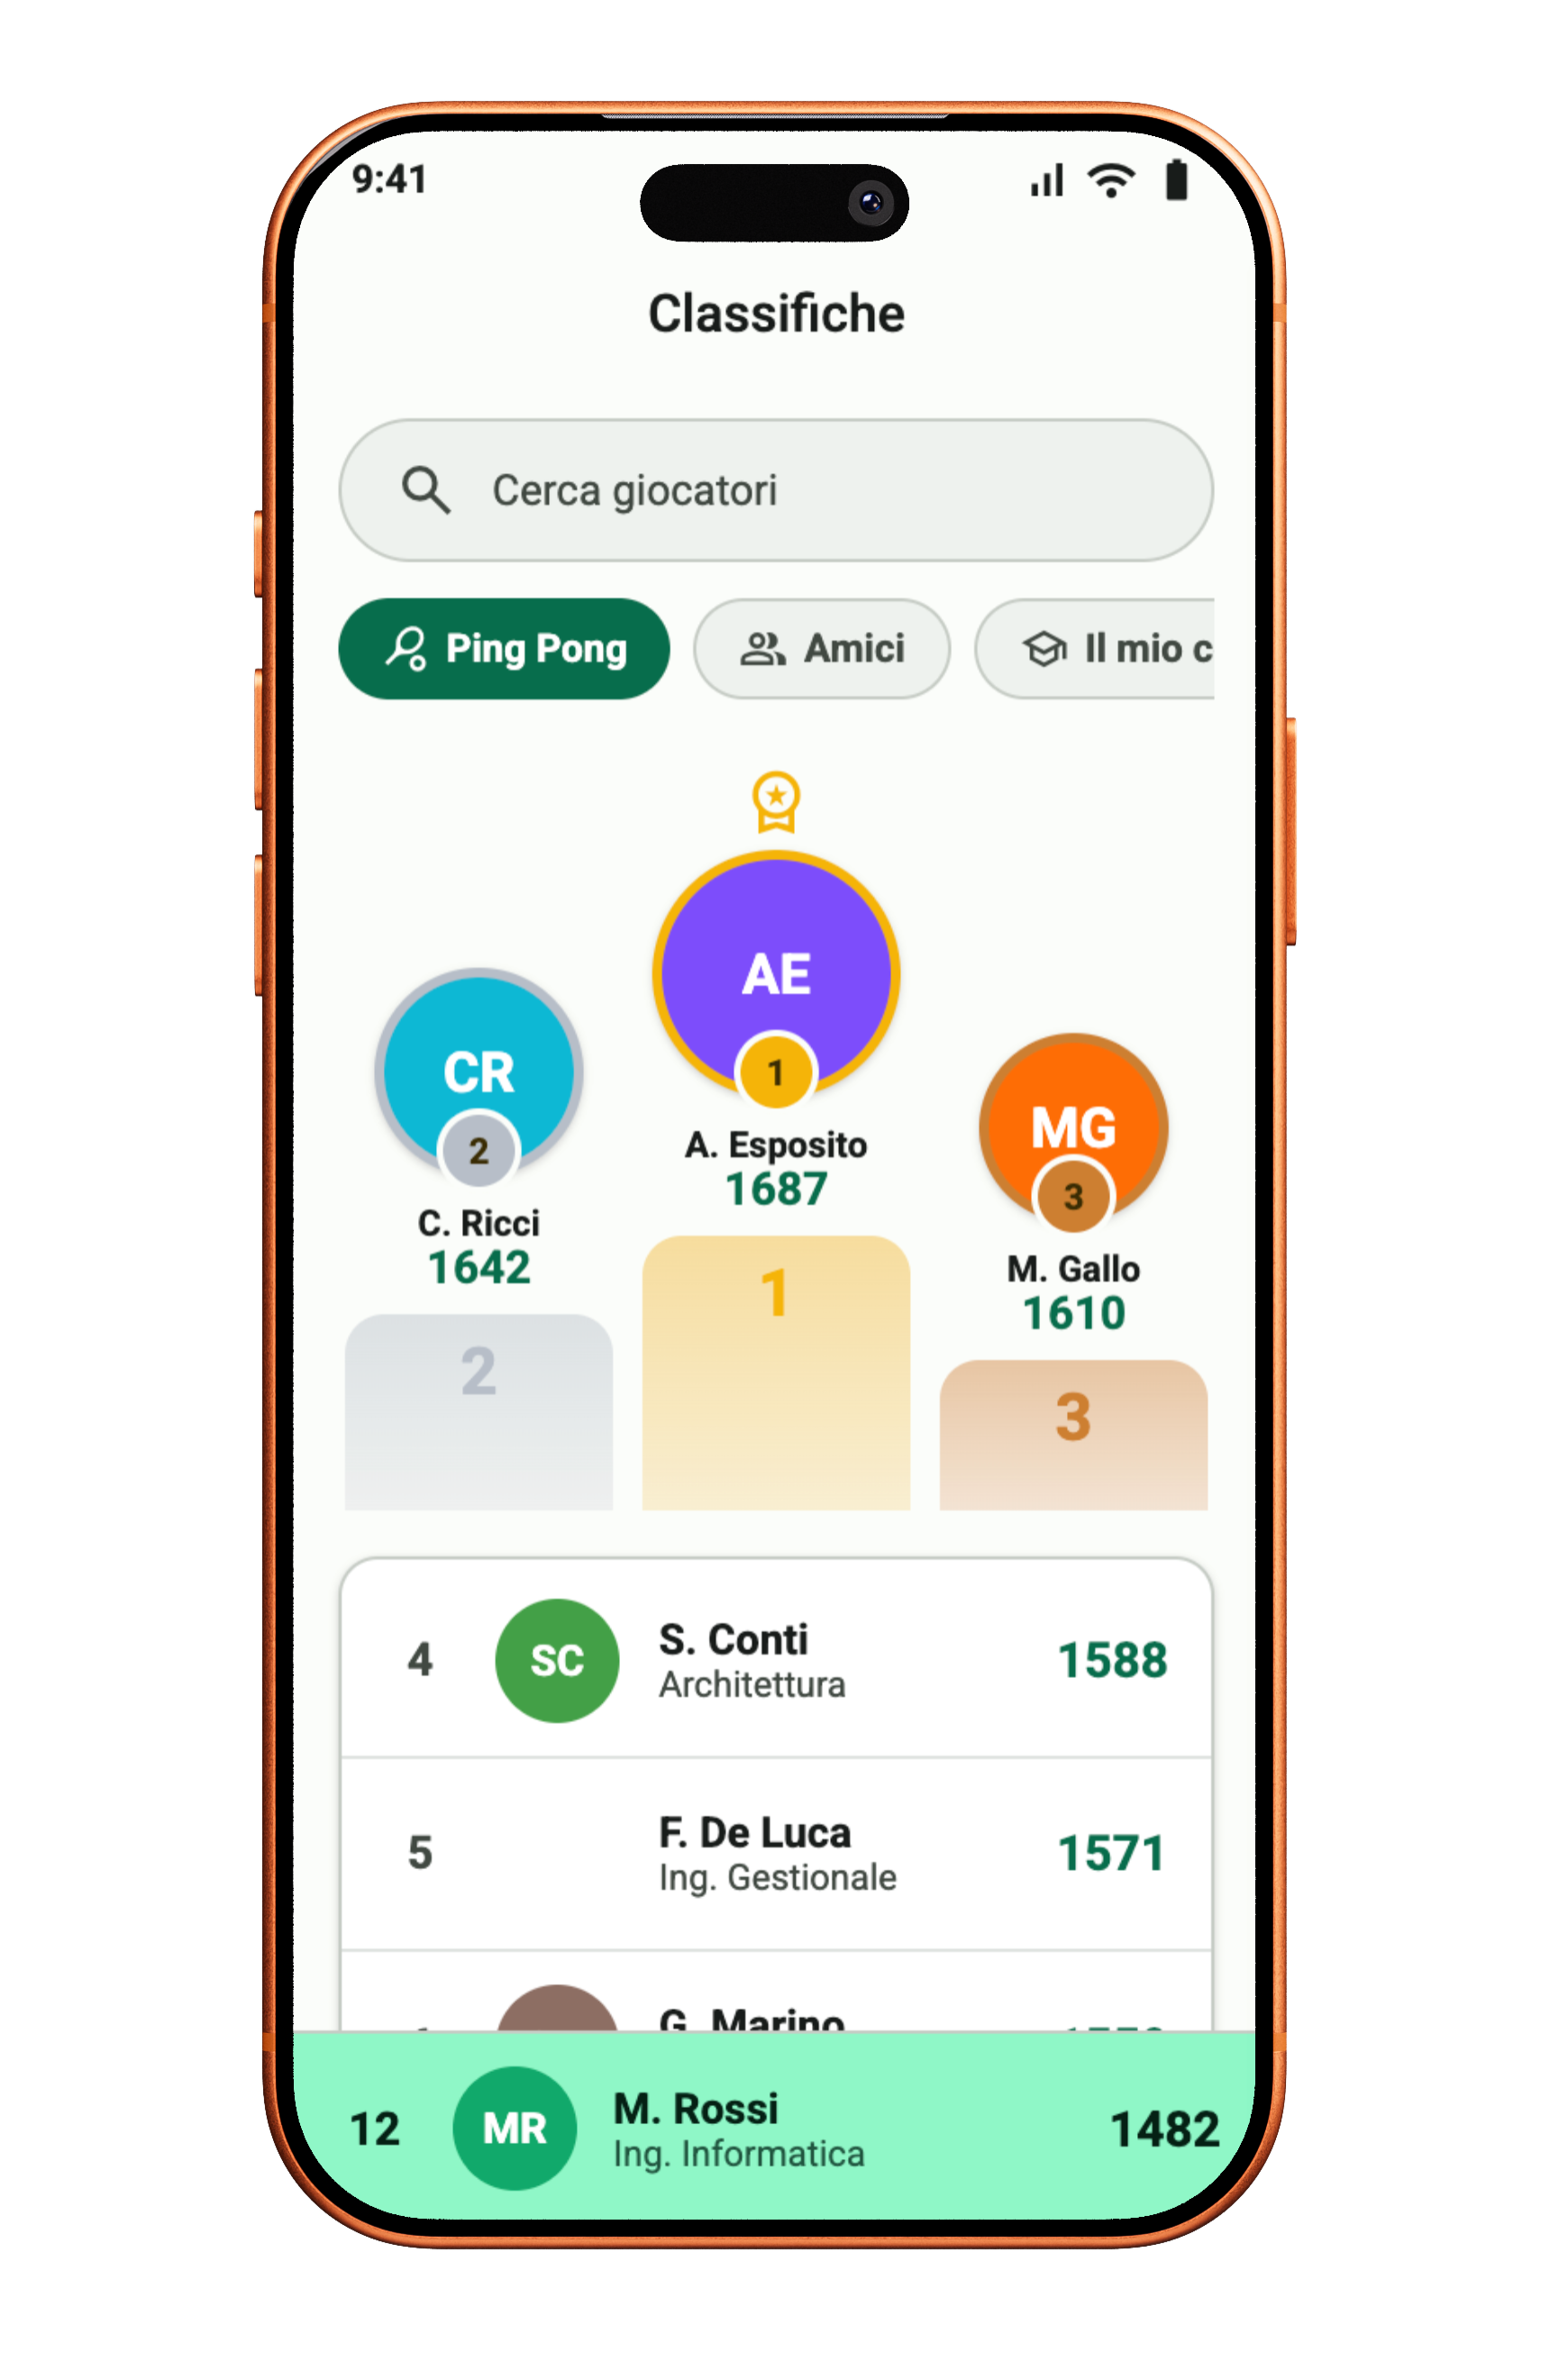
\includegraphics[width=0.25\linewidth]{mockups/leaderboard_it_light}}\hfill
    \subfloat[Friends]{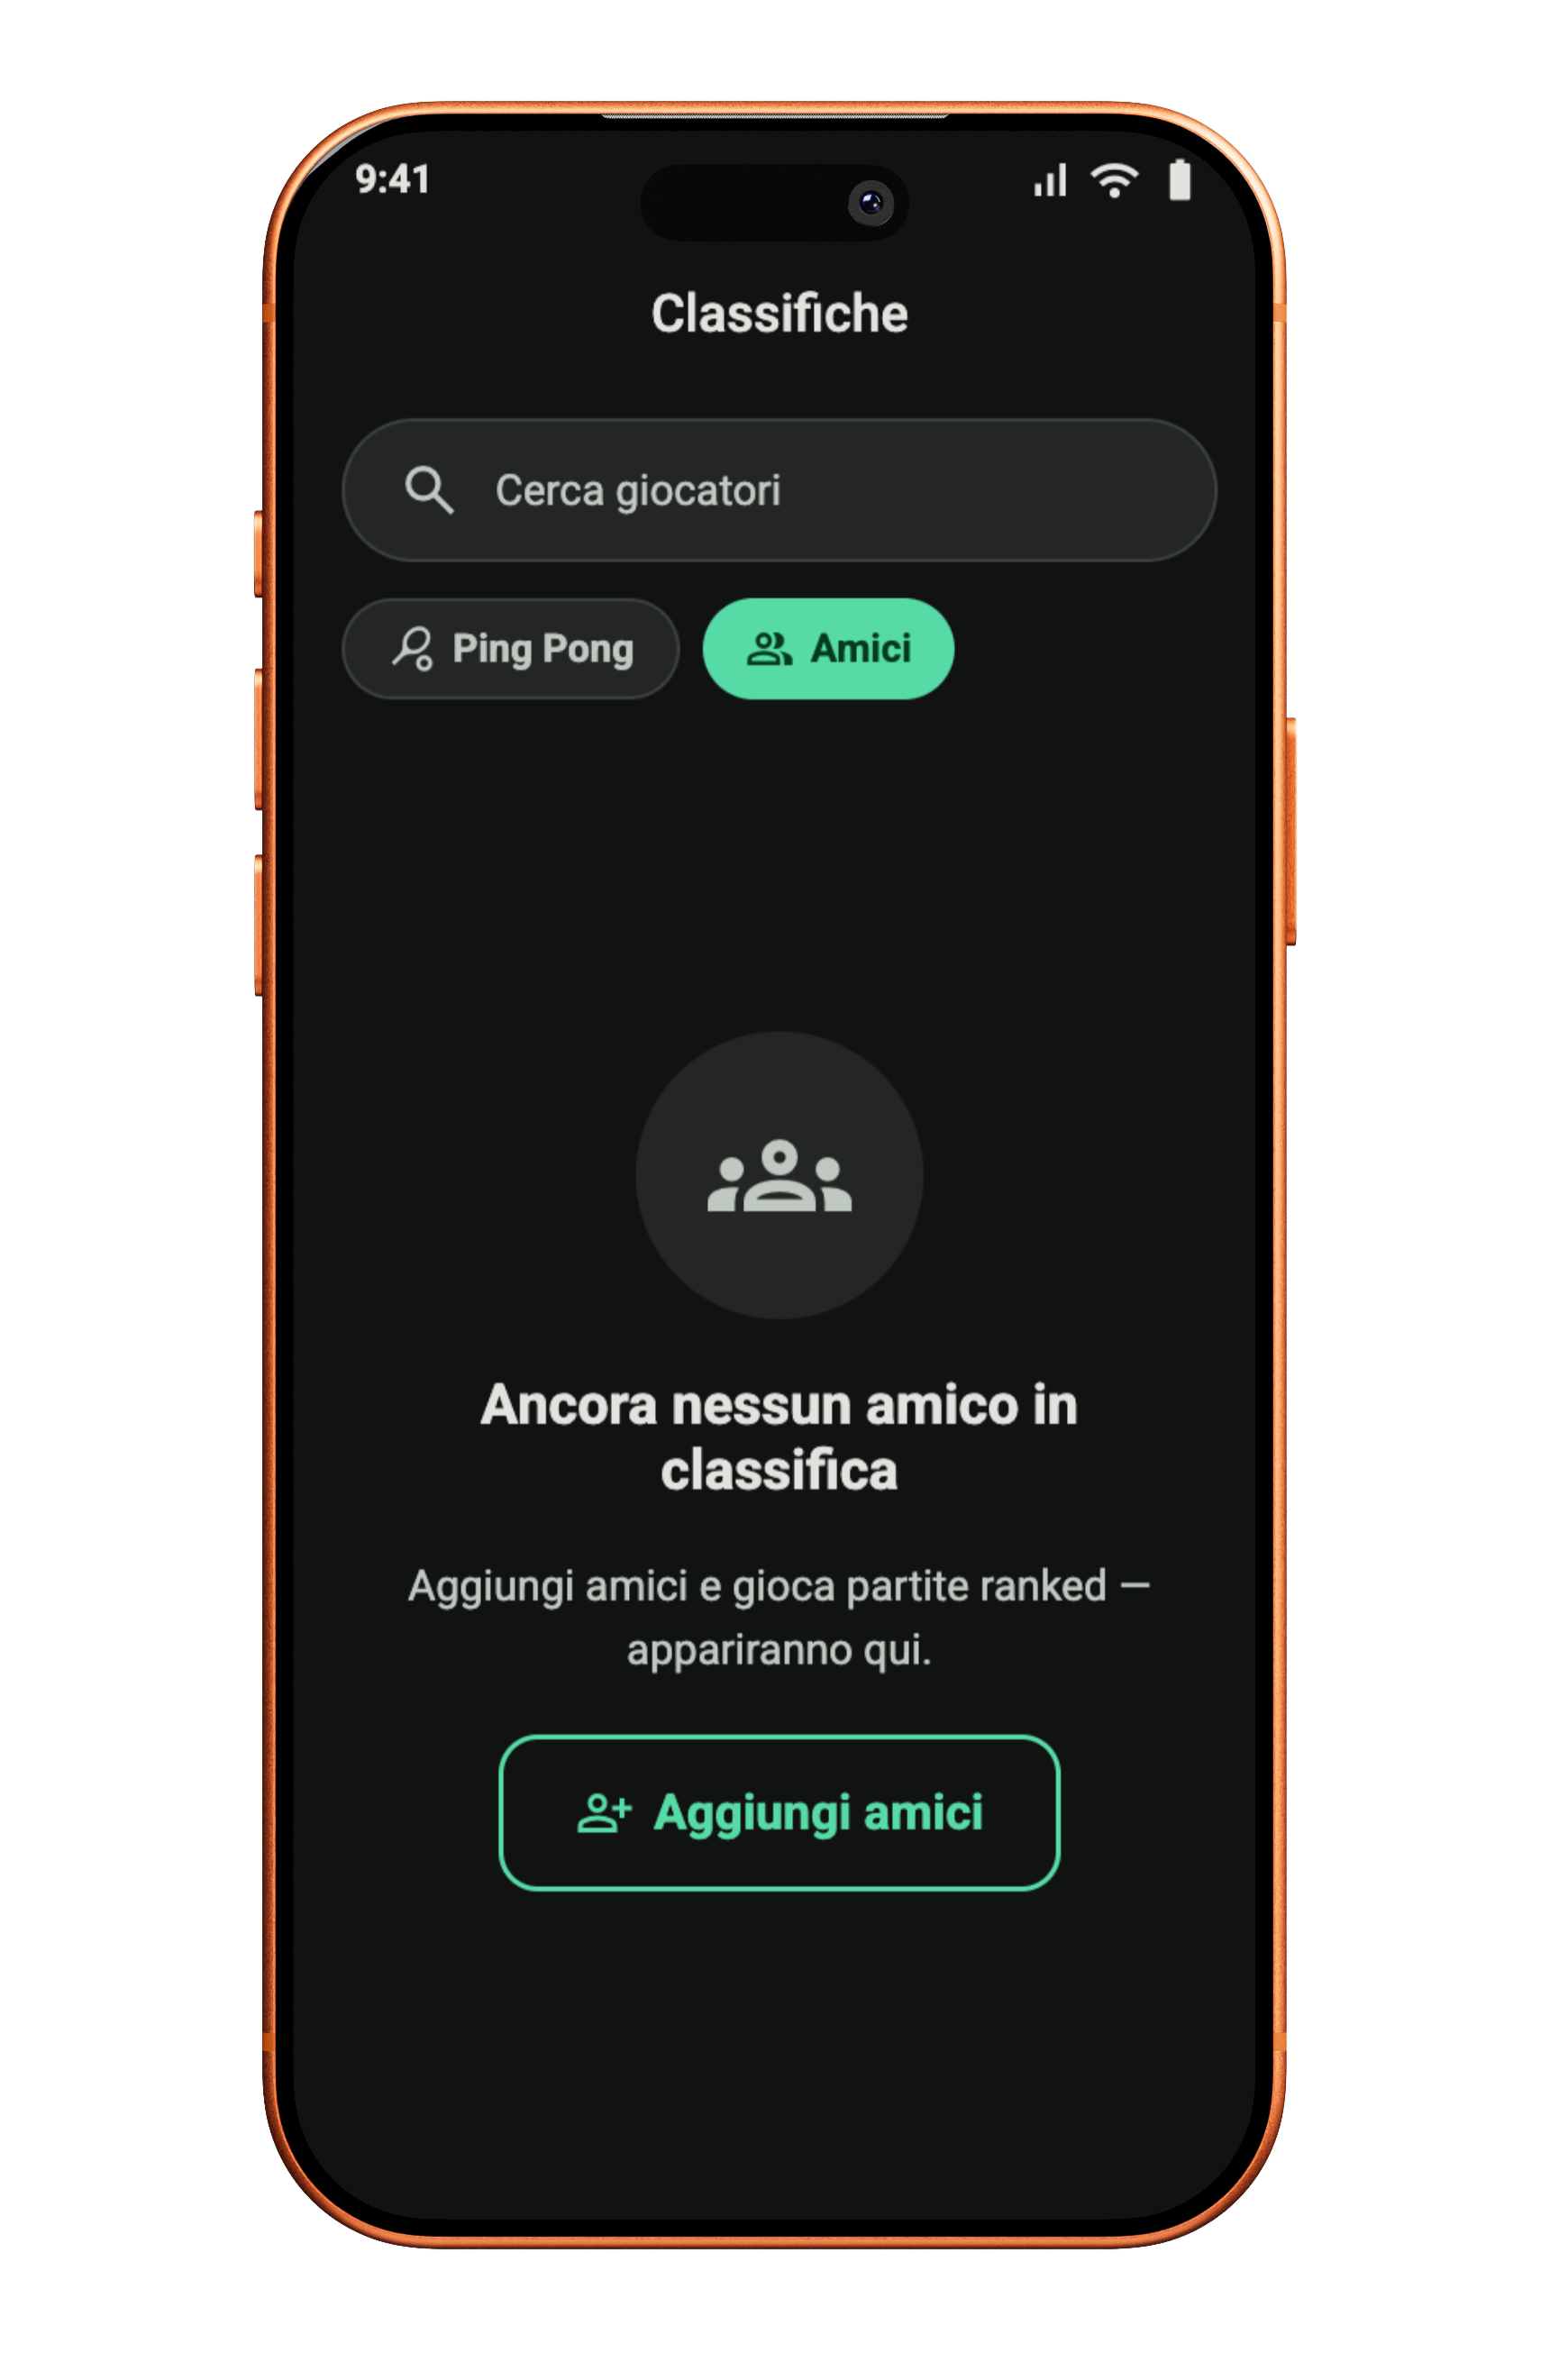
\includegraphics[width=0.25\linewidth]{mockups/friends_it_dark}}\hfill
    \subfloat[Settings]{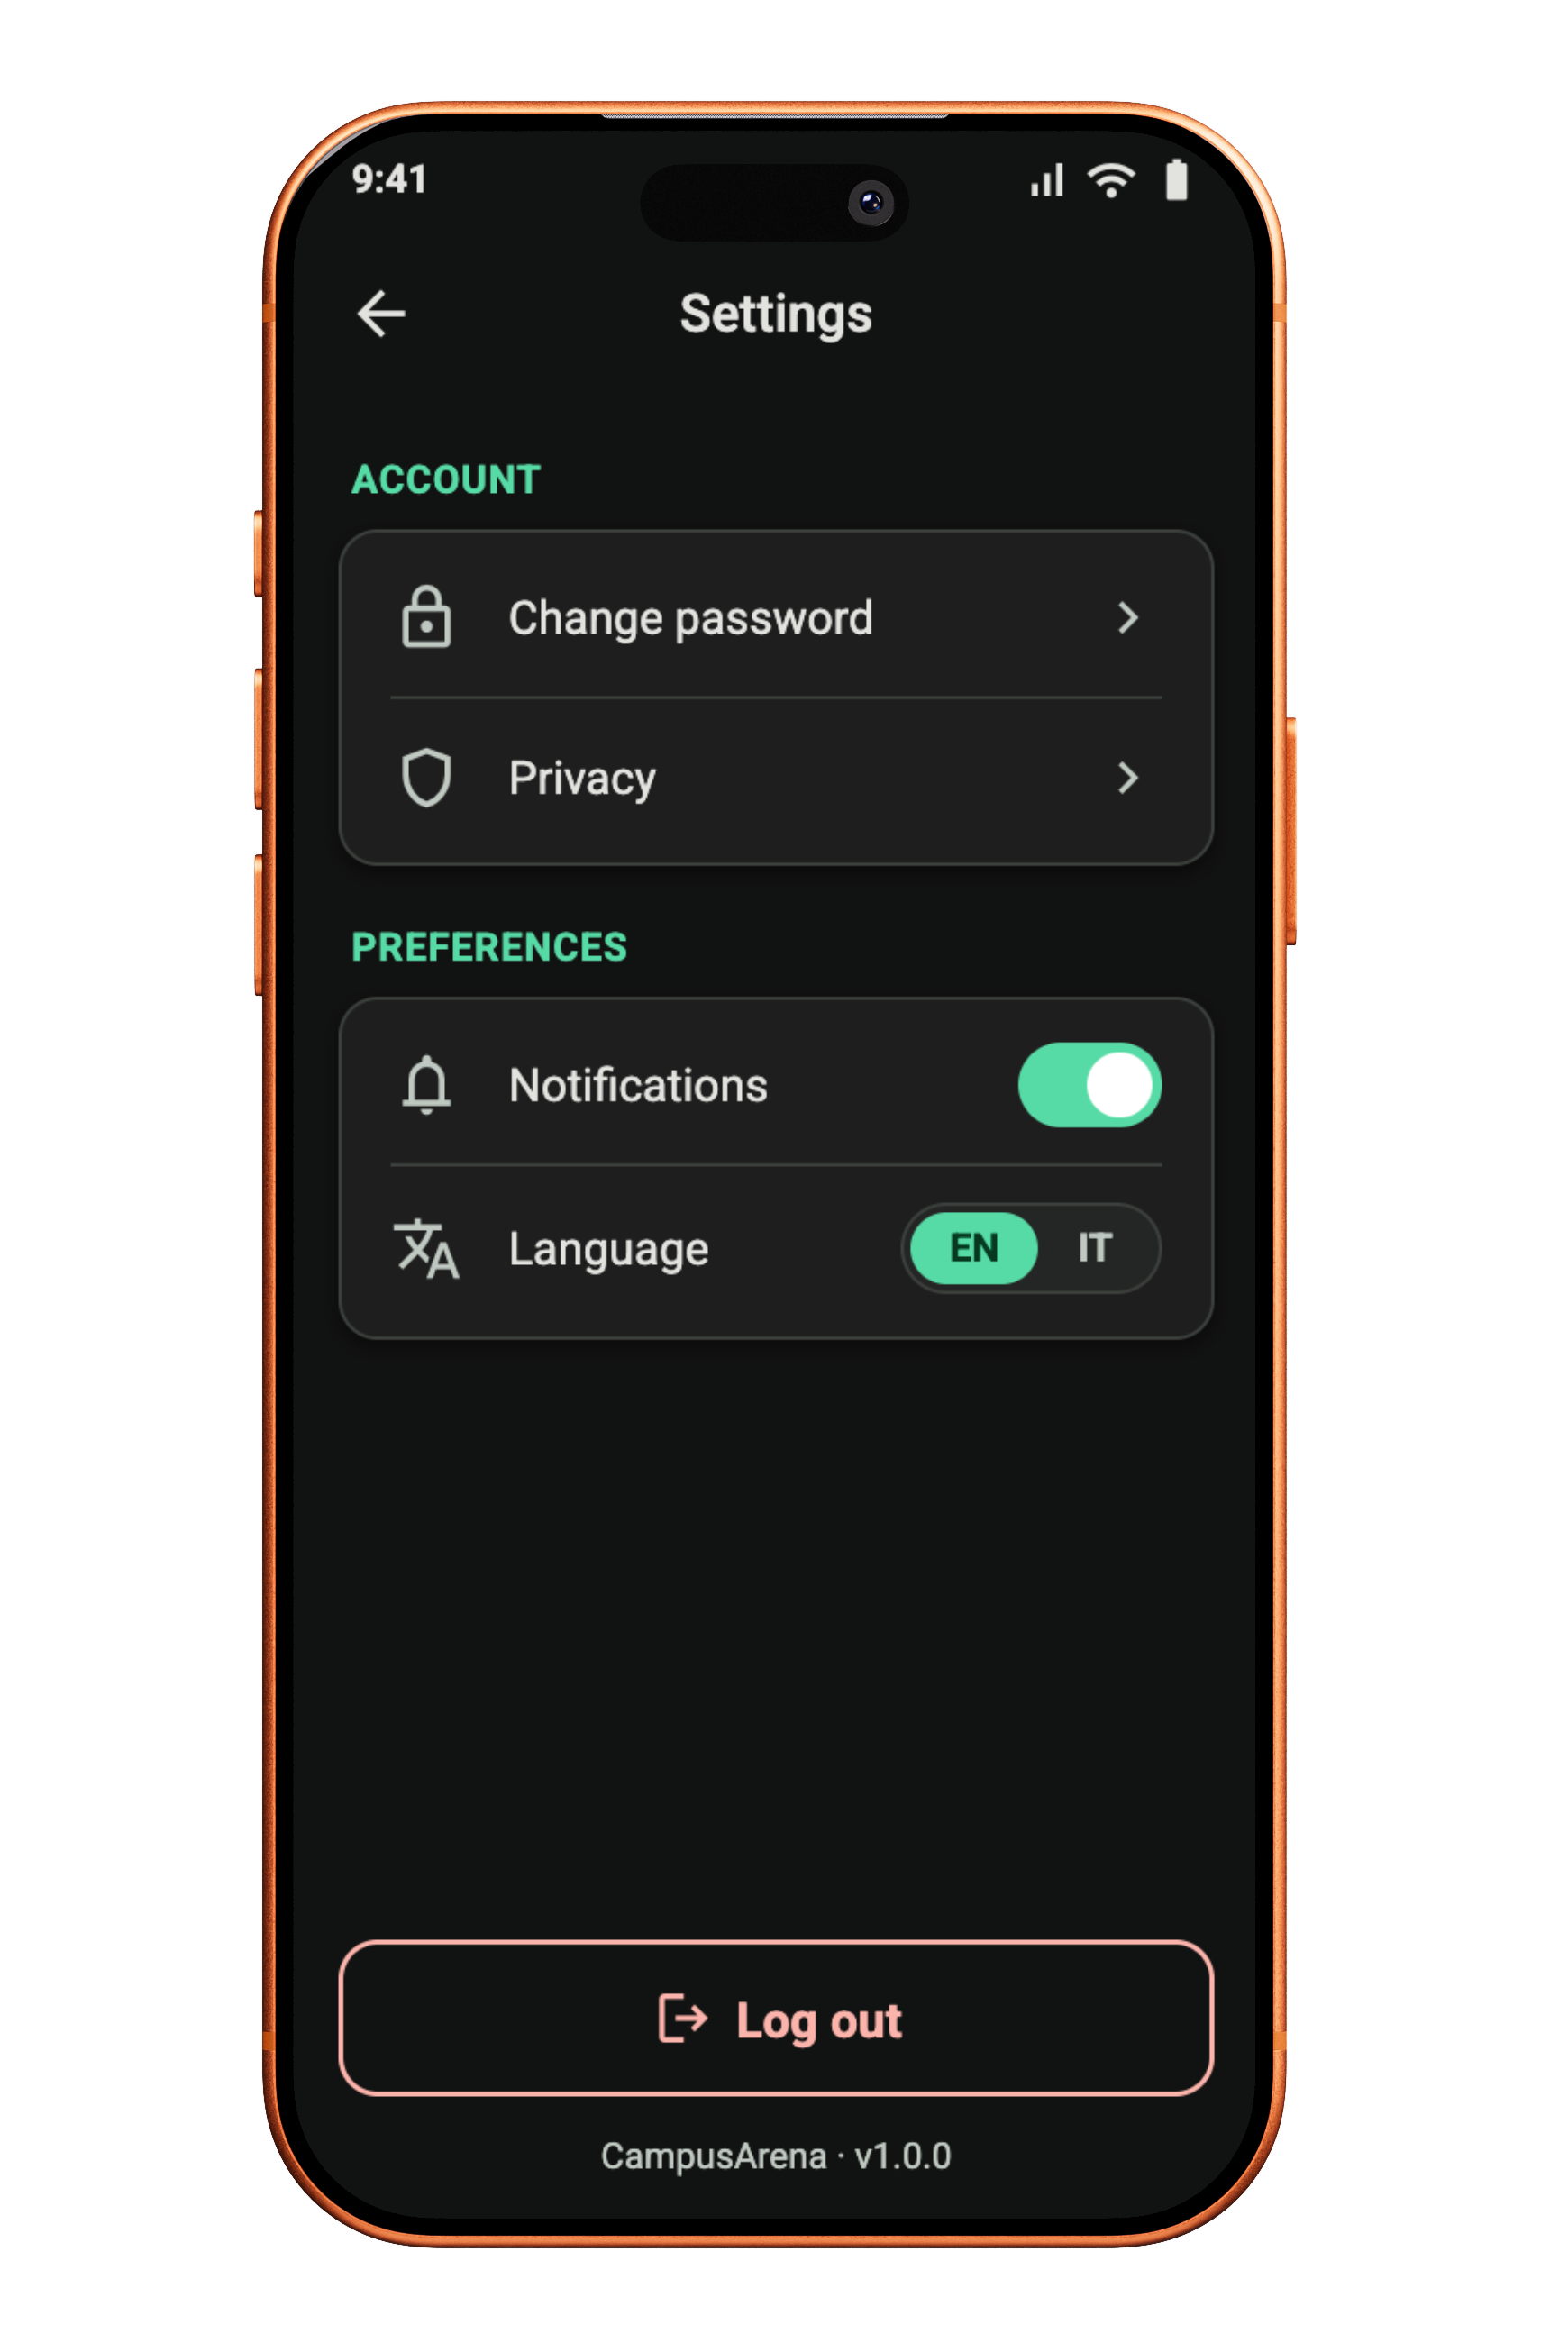
\includegraphics[width=0.25\linewidth]{mockups/settings_en_dark}}\hfill
    \subfloat[Profile \& stats]{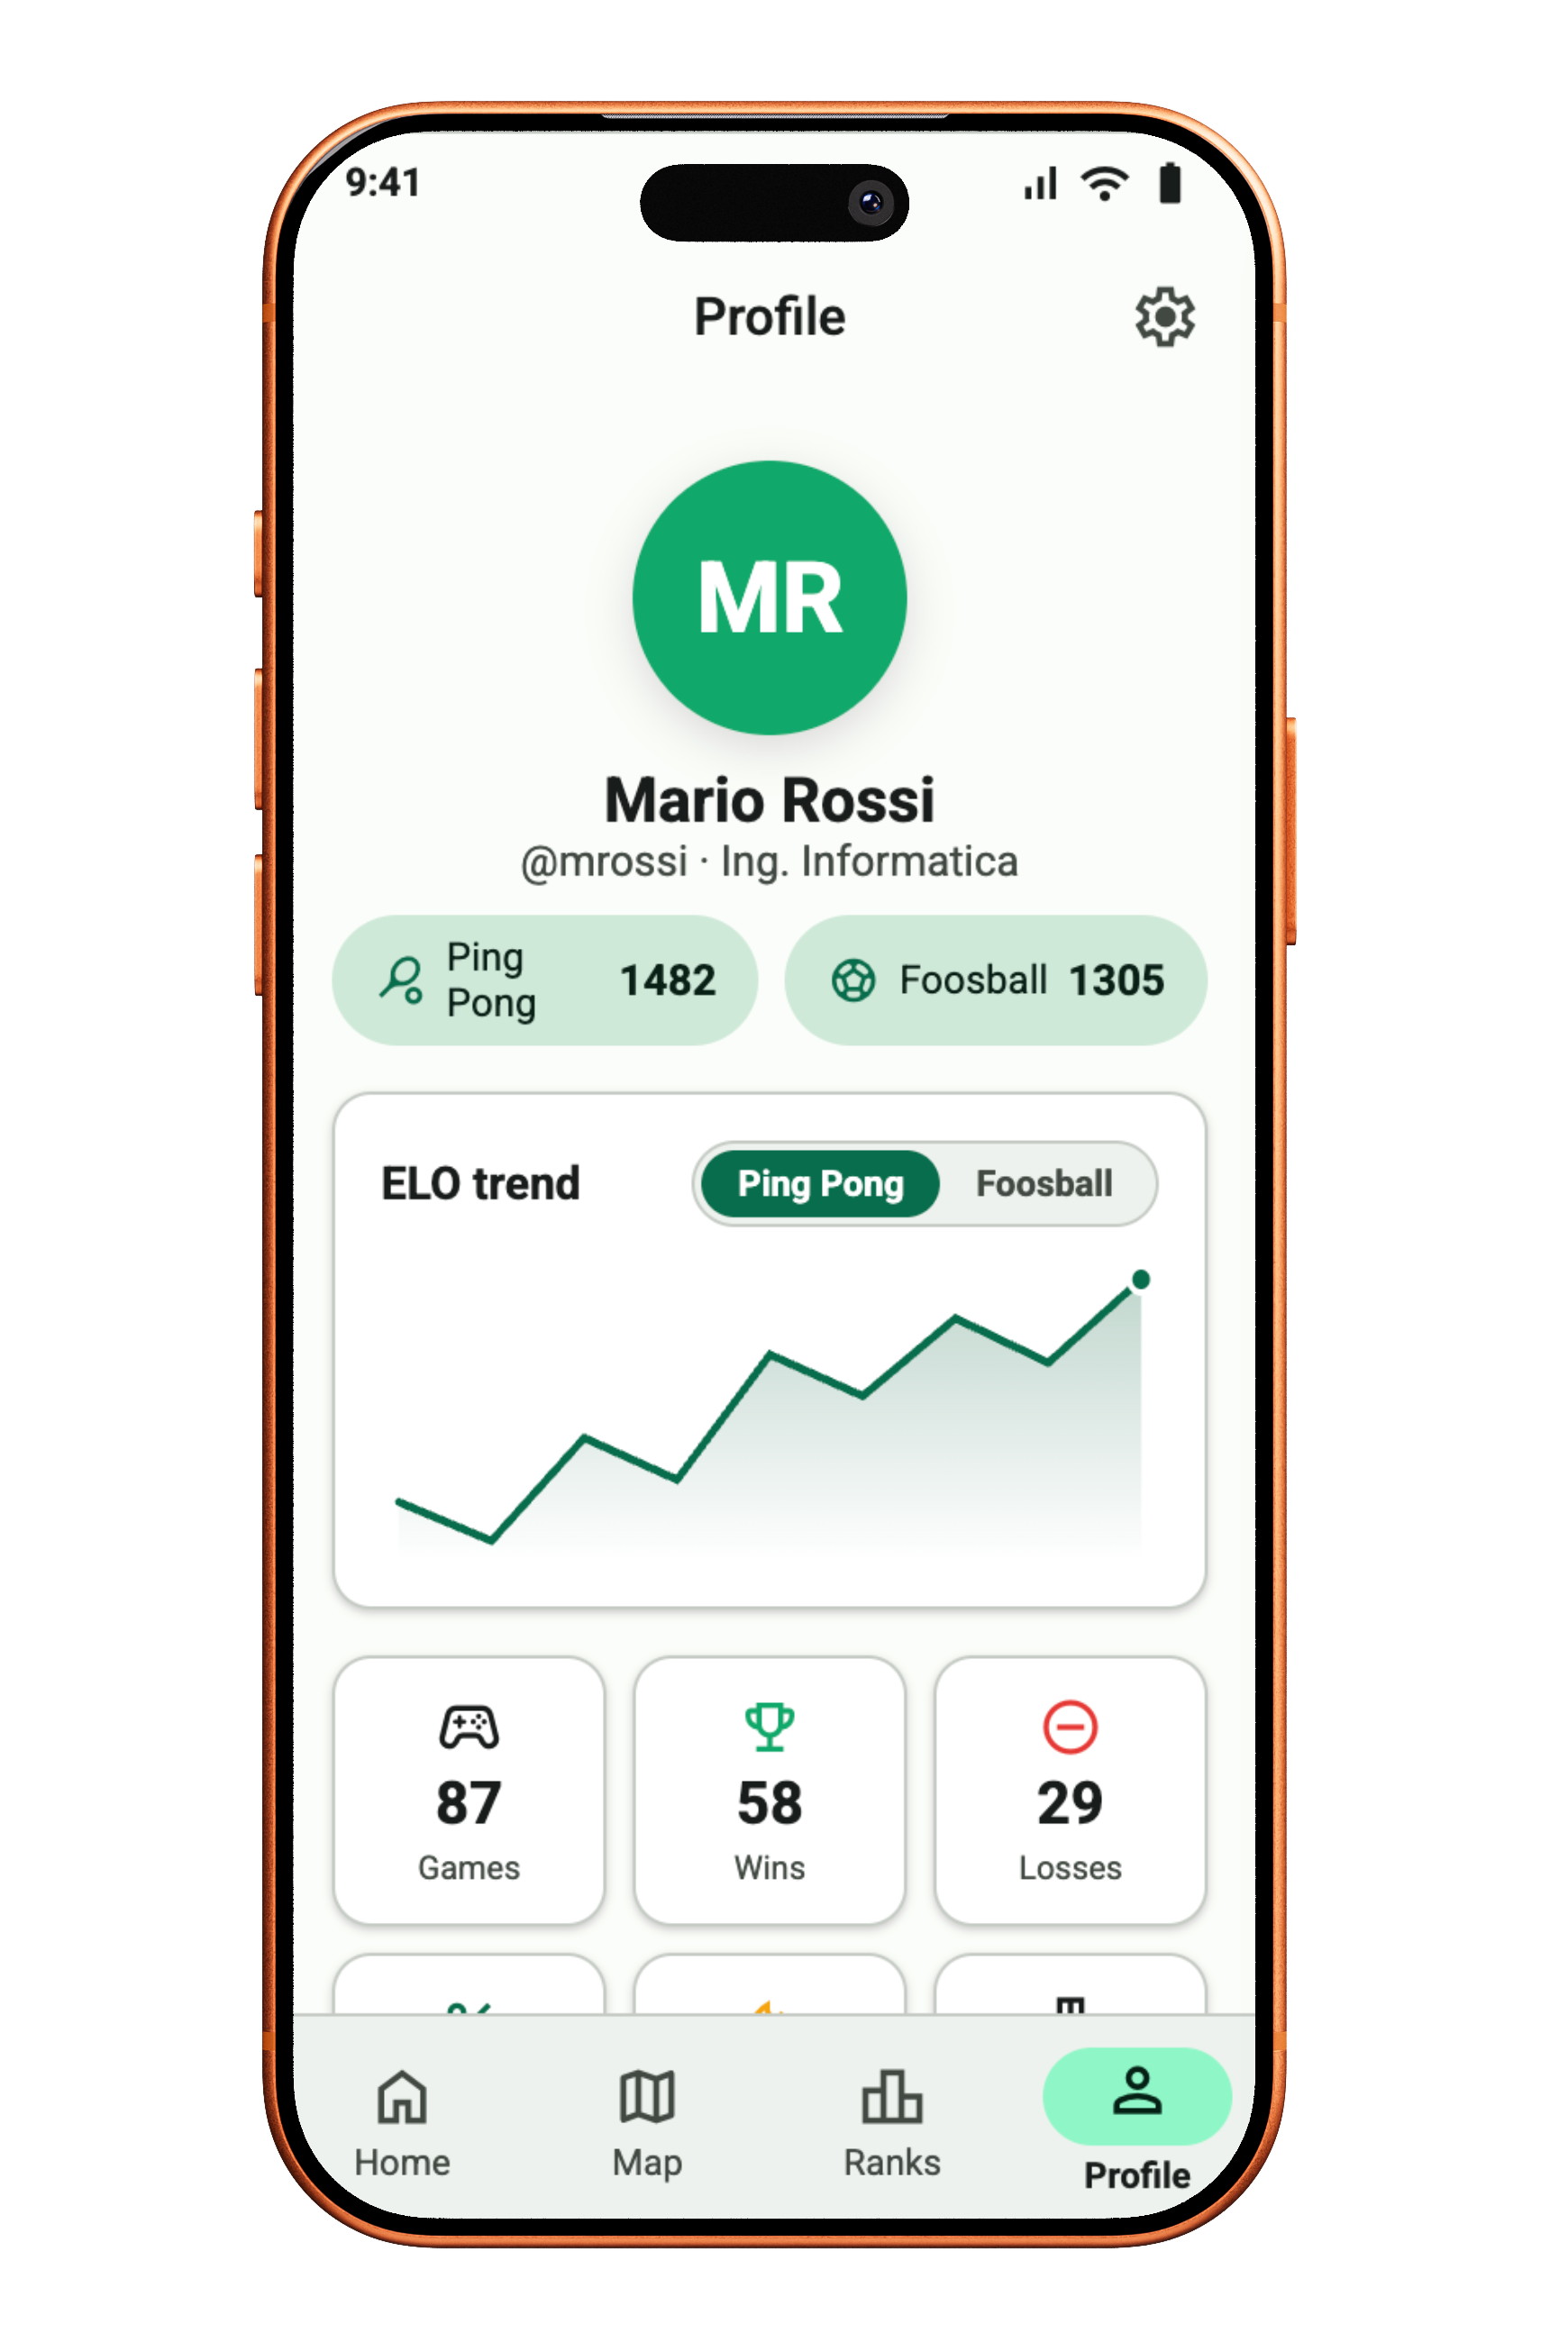
\includegraphics[width=0.25\linewidth]{mockups/profile_en_light}}
    \caption{Leaderboards (global / per-sport / friends / course-rivalry), the friends screen, account settings, and the player profile.}
    \label{fig:lead_profile_screens}
\end{figure}

\begin{figure}[H]
    \centering
    \subfloat[Tournament browser]{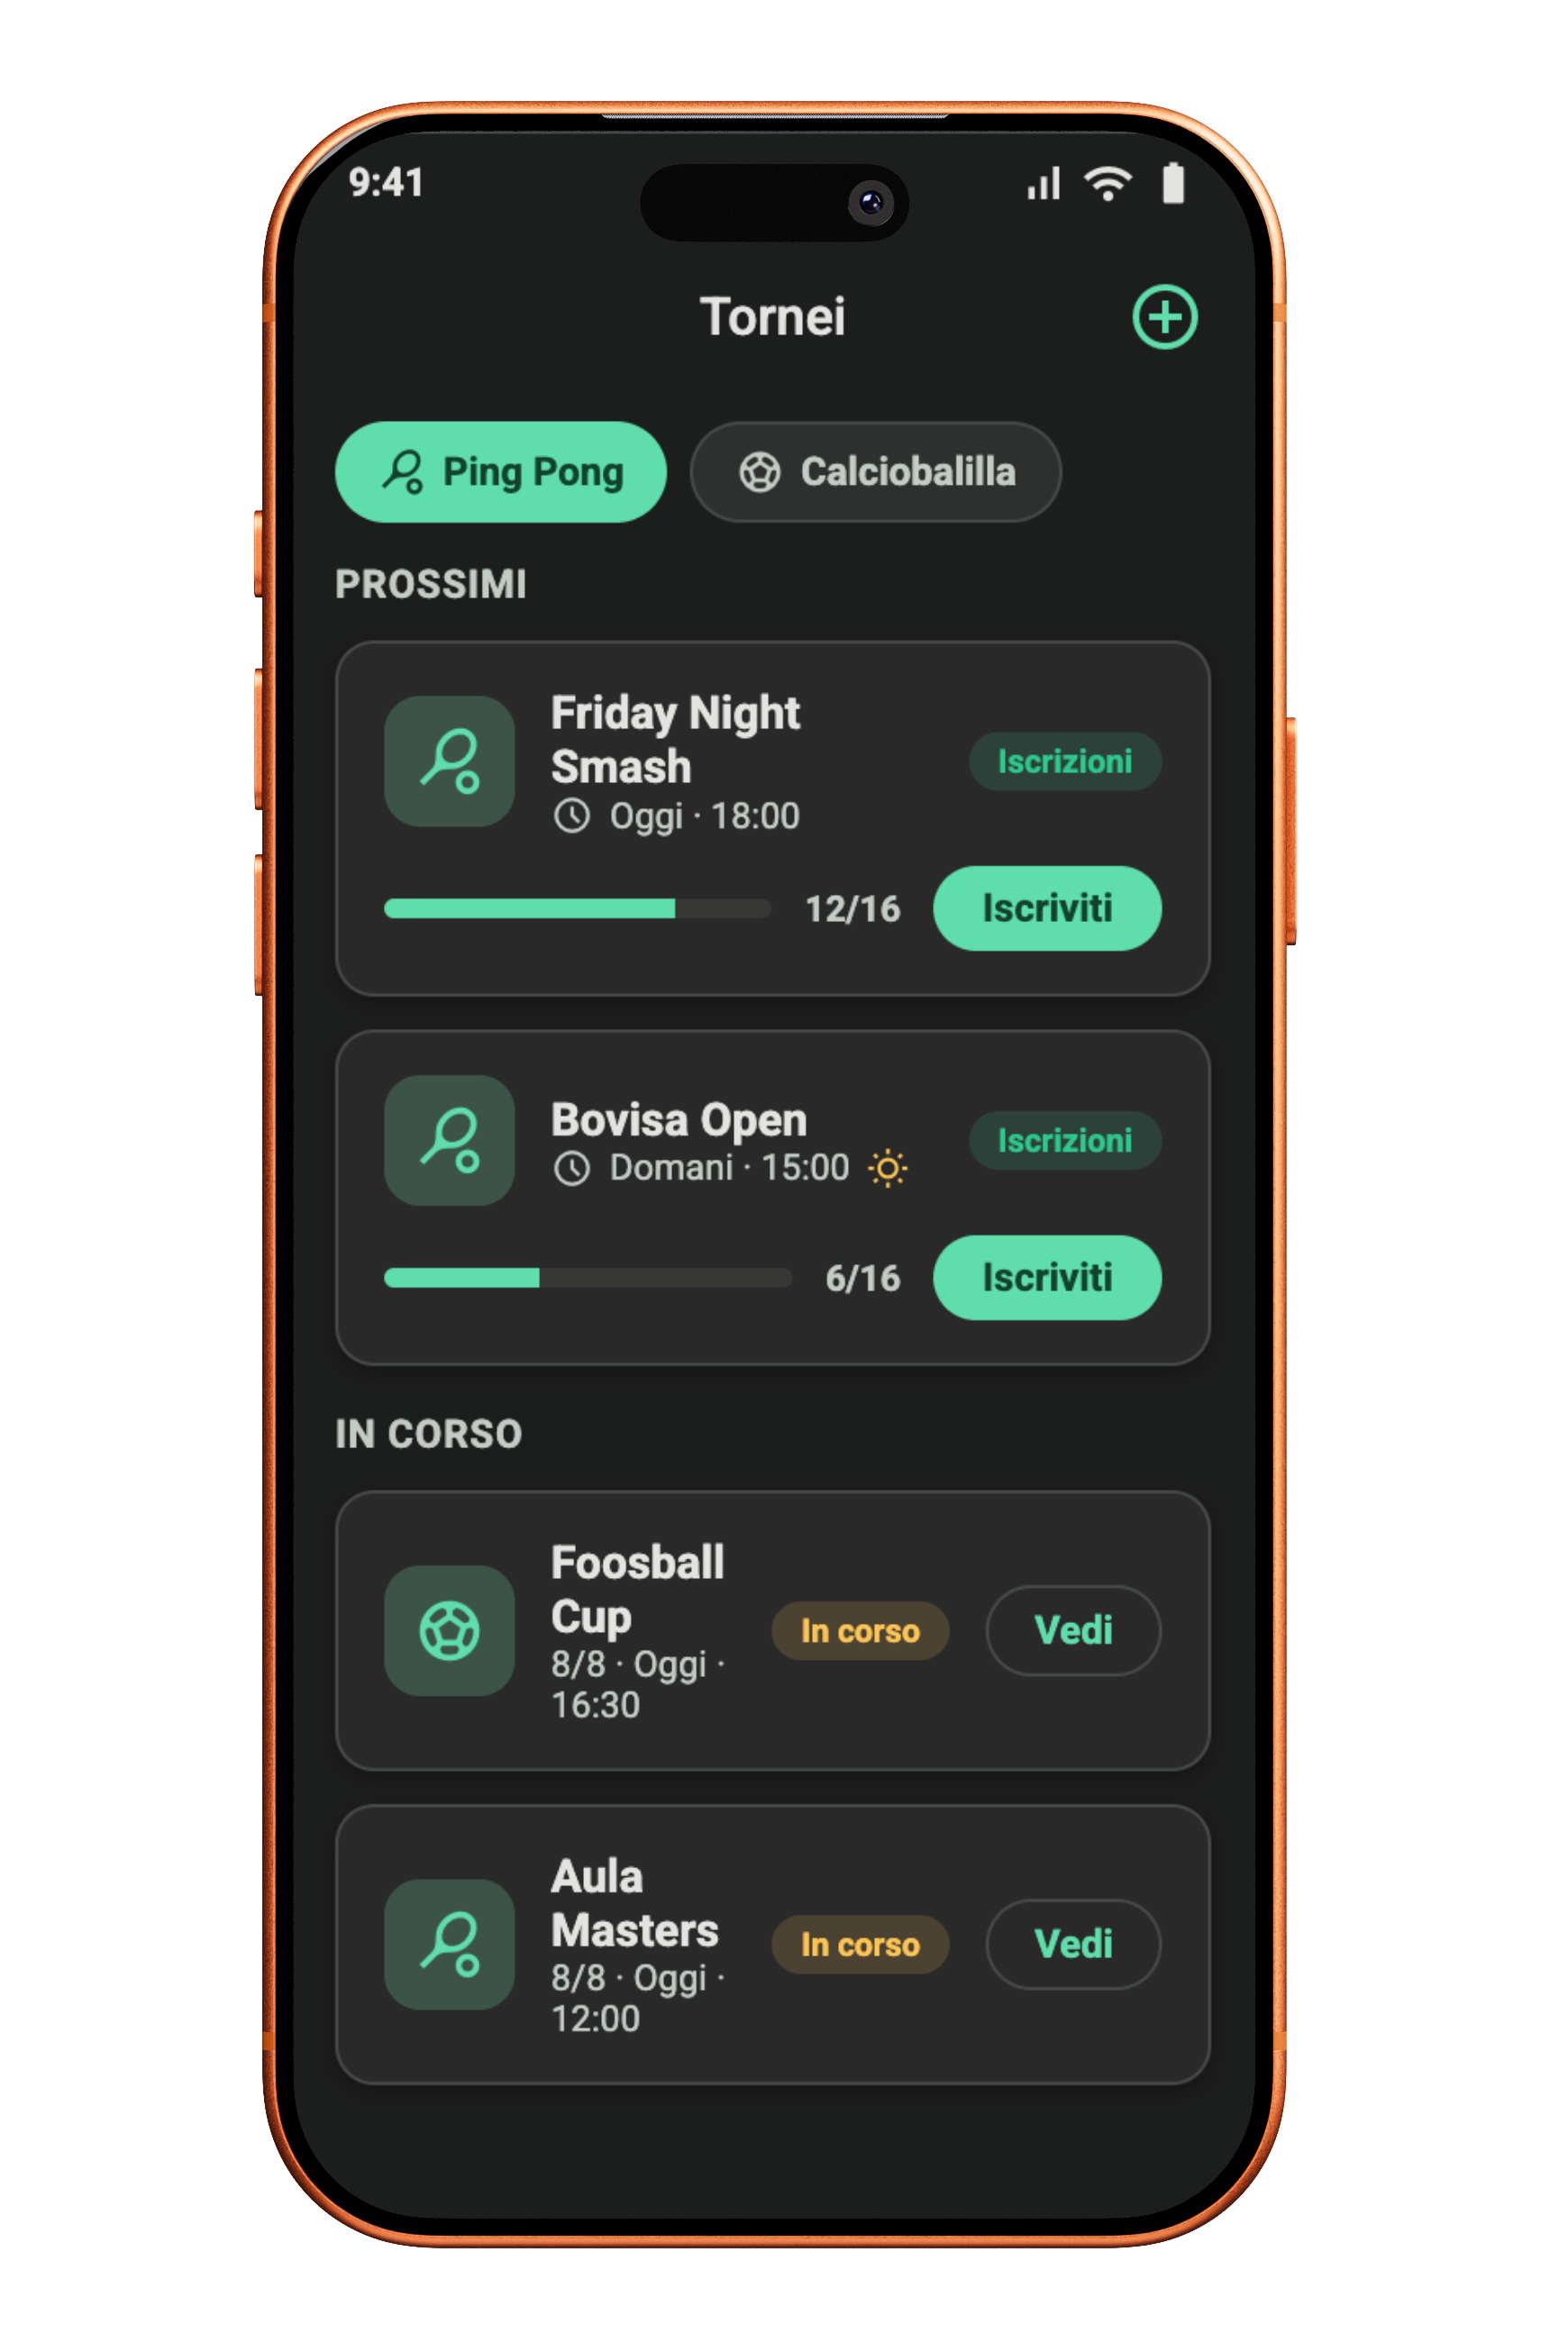
\includegraphics[width=0.25\linewidth]{mockups/tournaments_it_dark}}\hfill
    \subfloat[Create tournament]{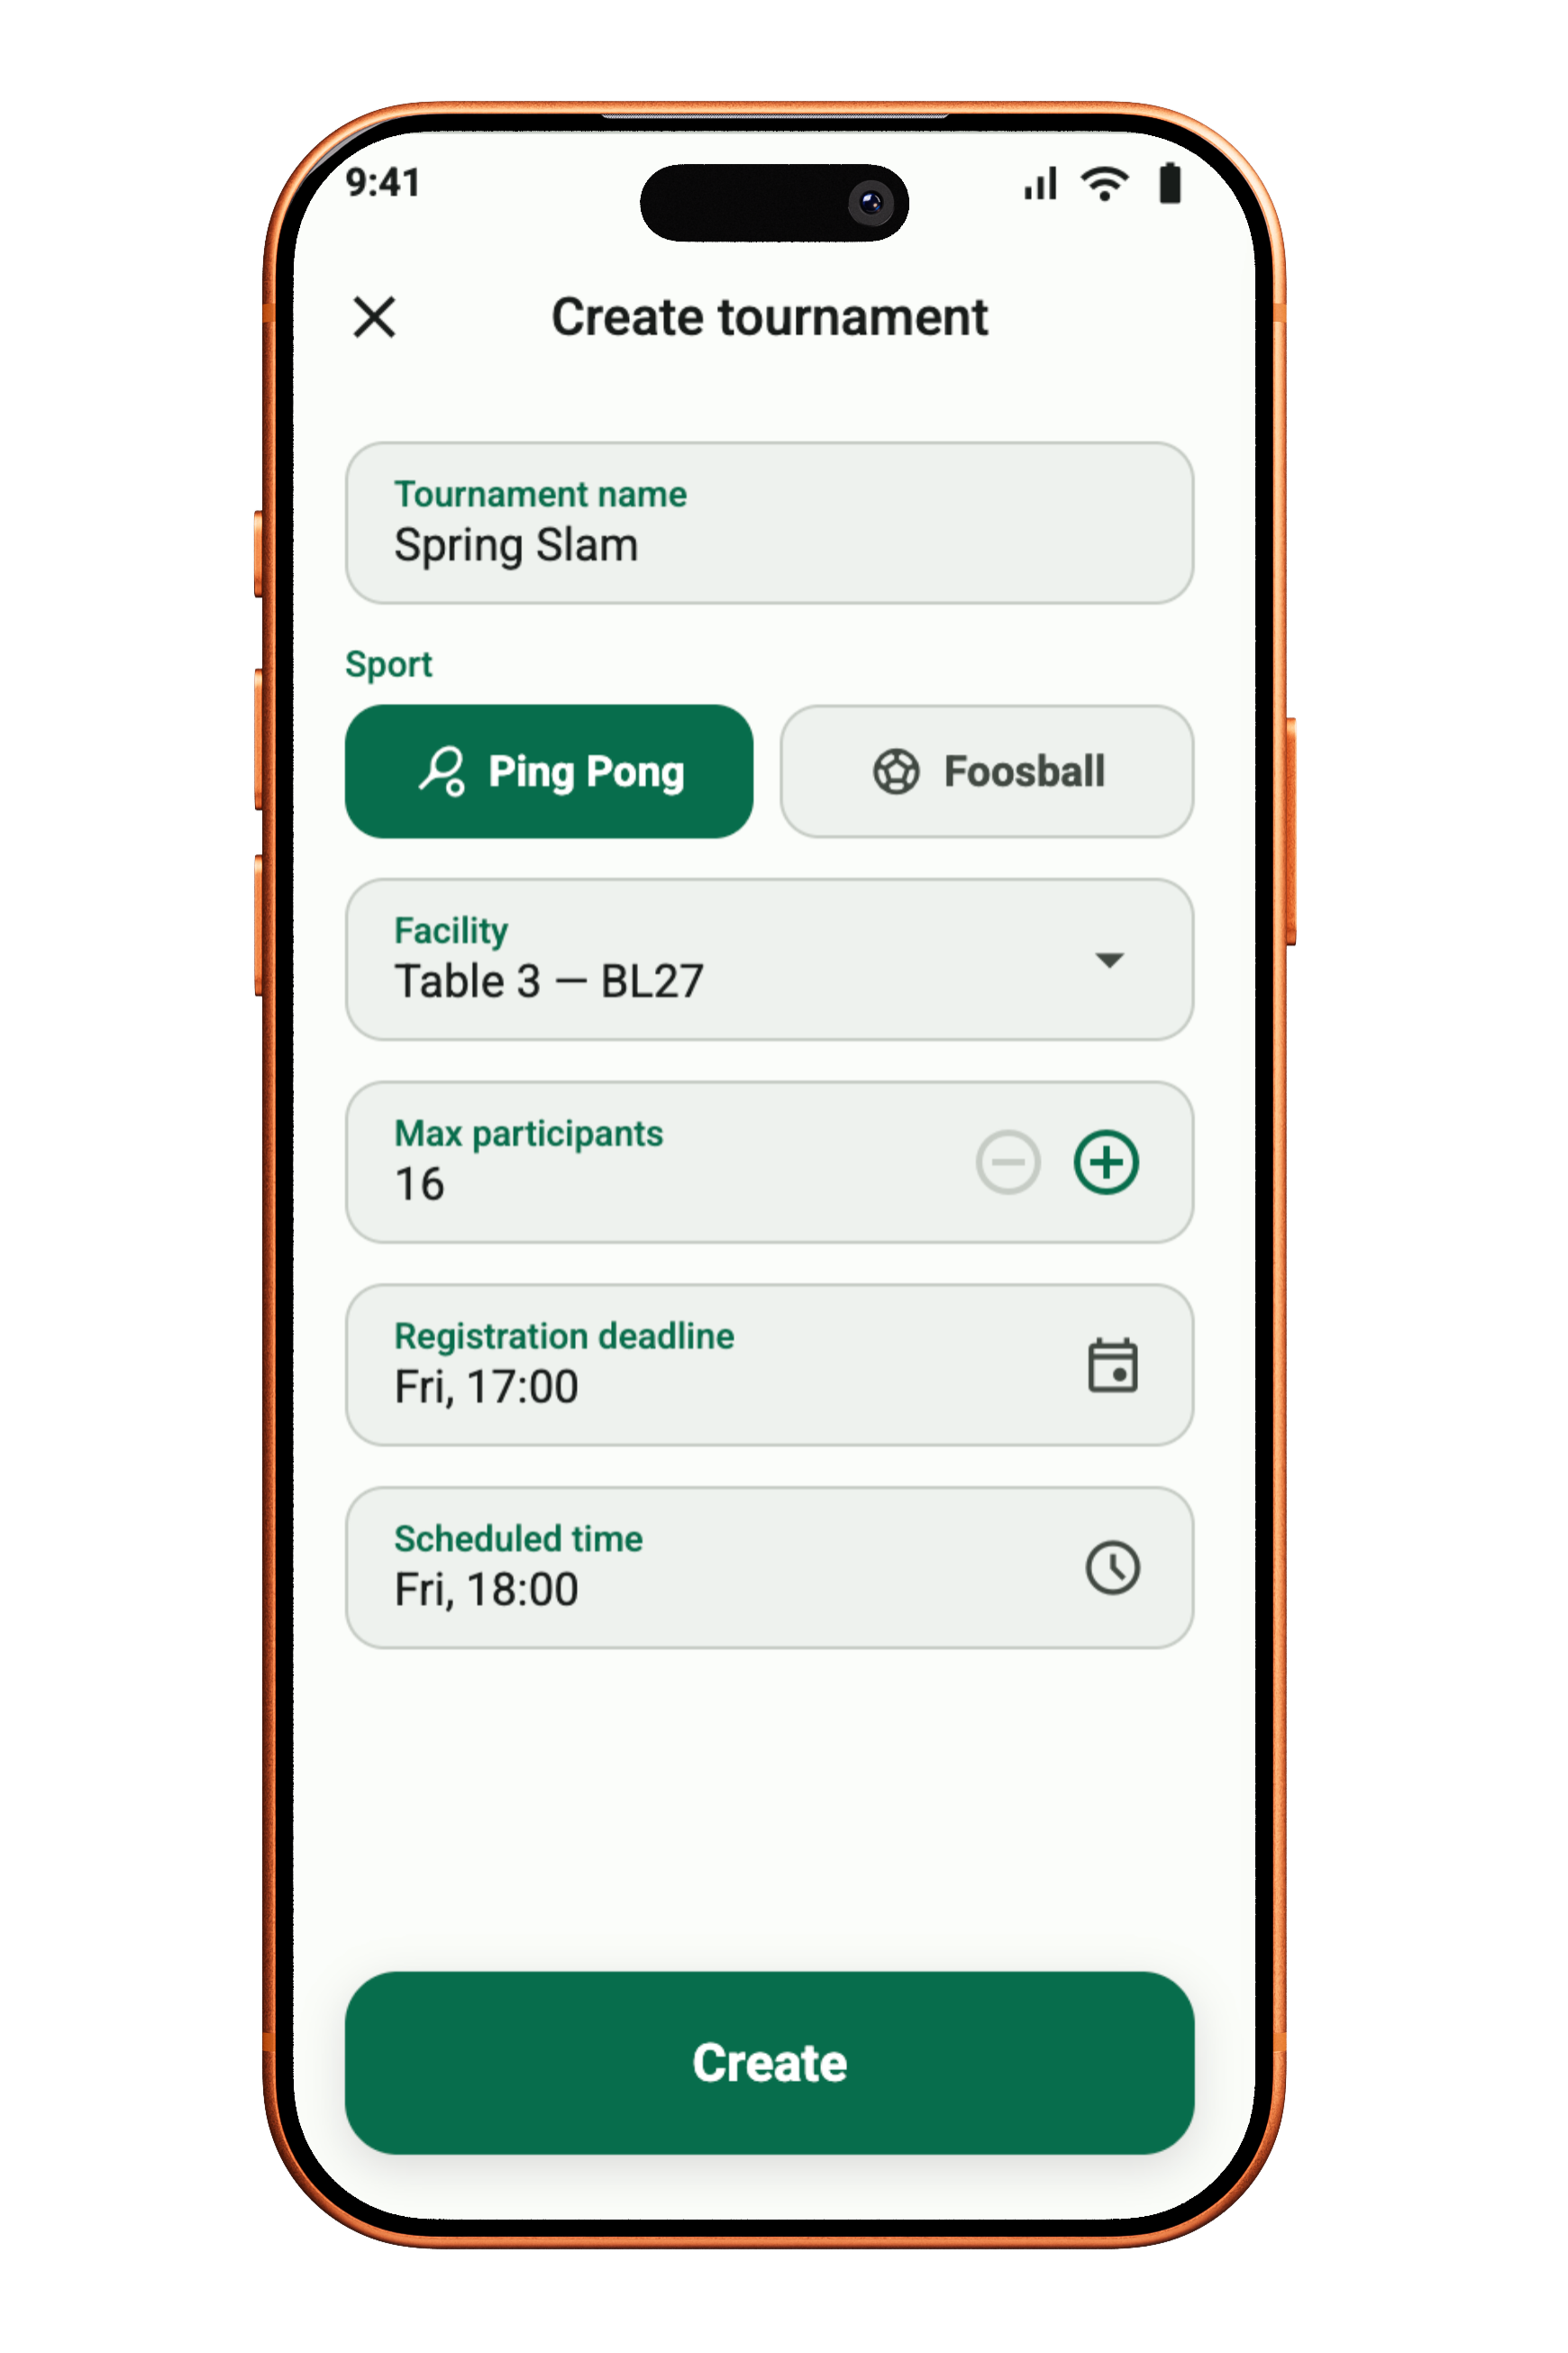
\includegraphics[width=0.25\linewidth]{mockups/create_en_light}}\hfill
    \subfloat[Live bracket]{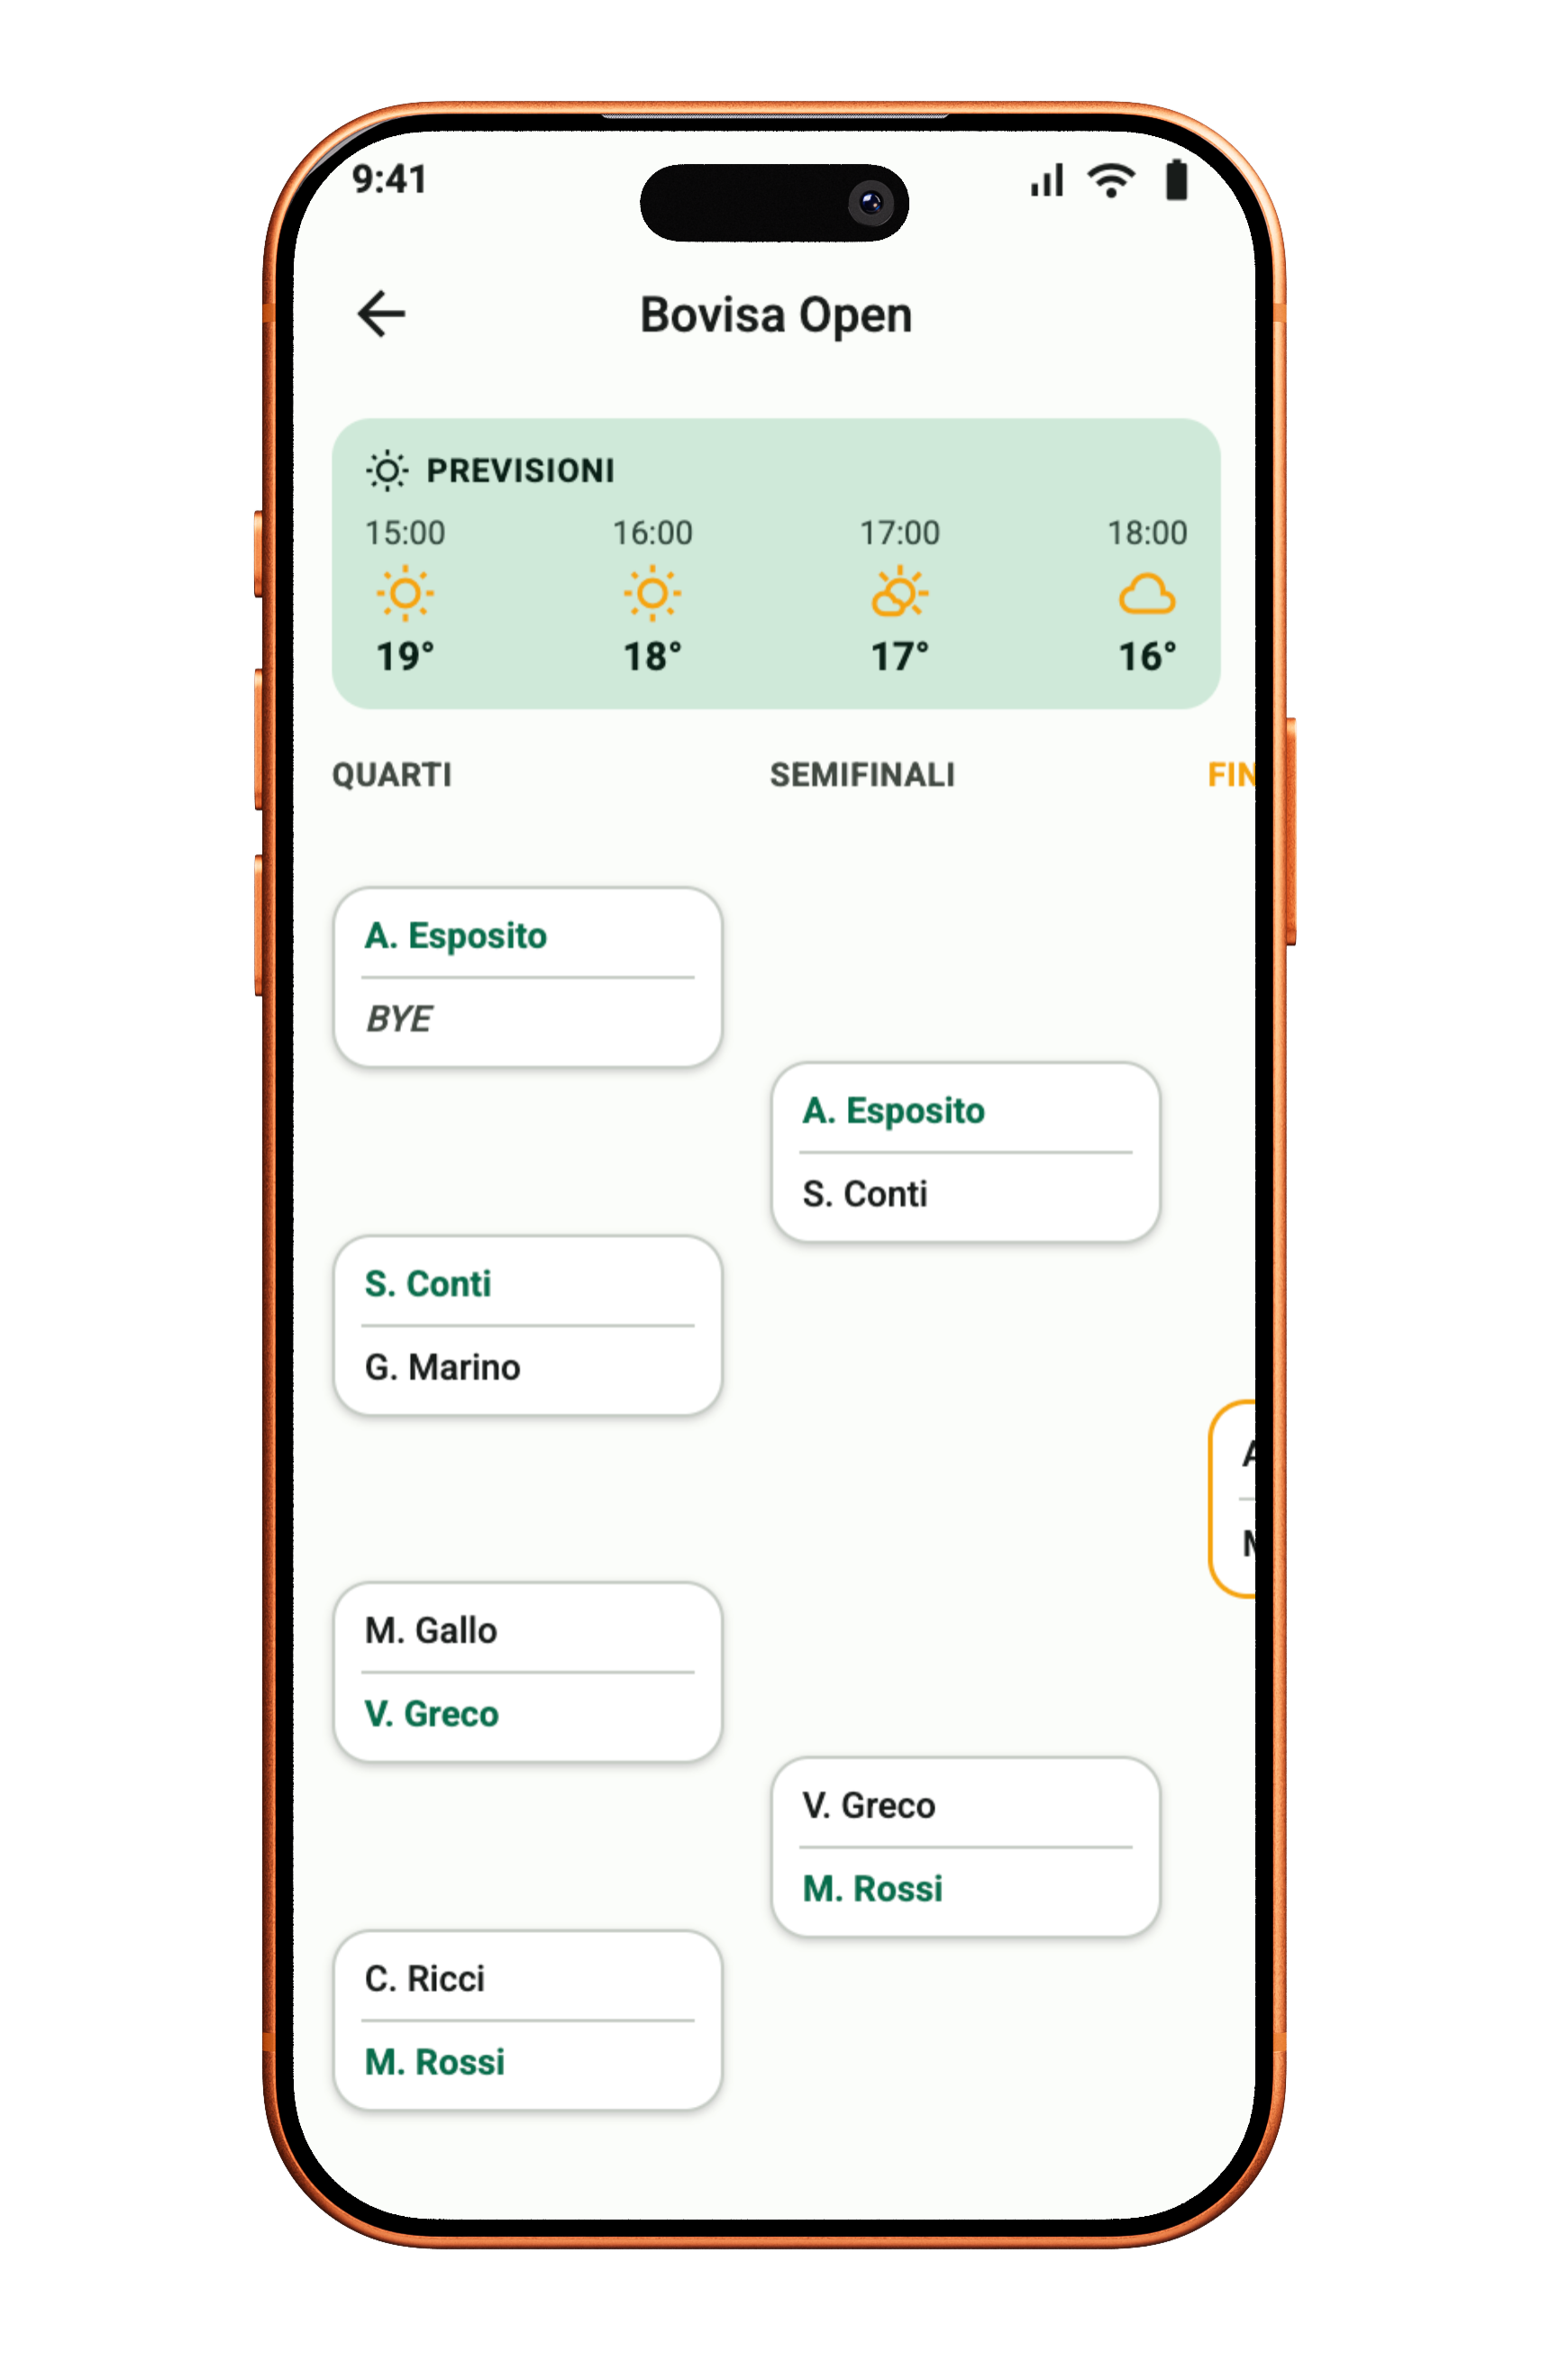
\includegraphics[width=0.25\linewidth]{mockups/bracket_it_light}}\hfill
    \subfloat[Tournament detail]{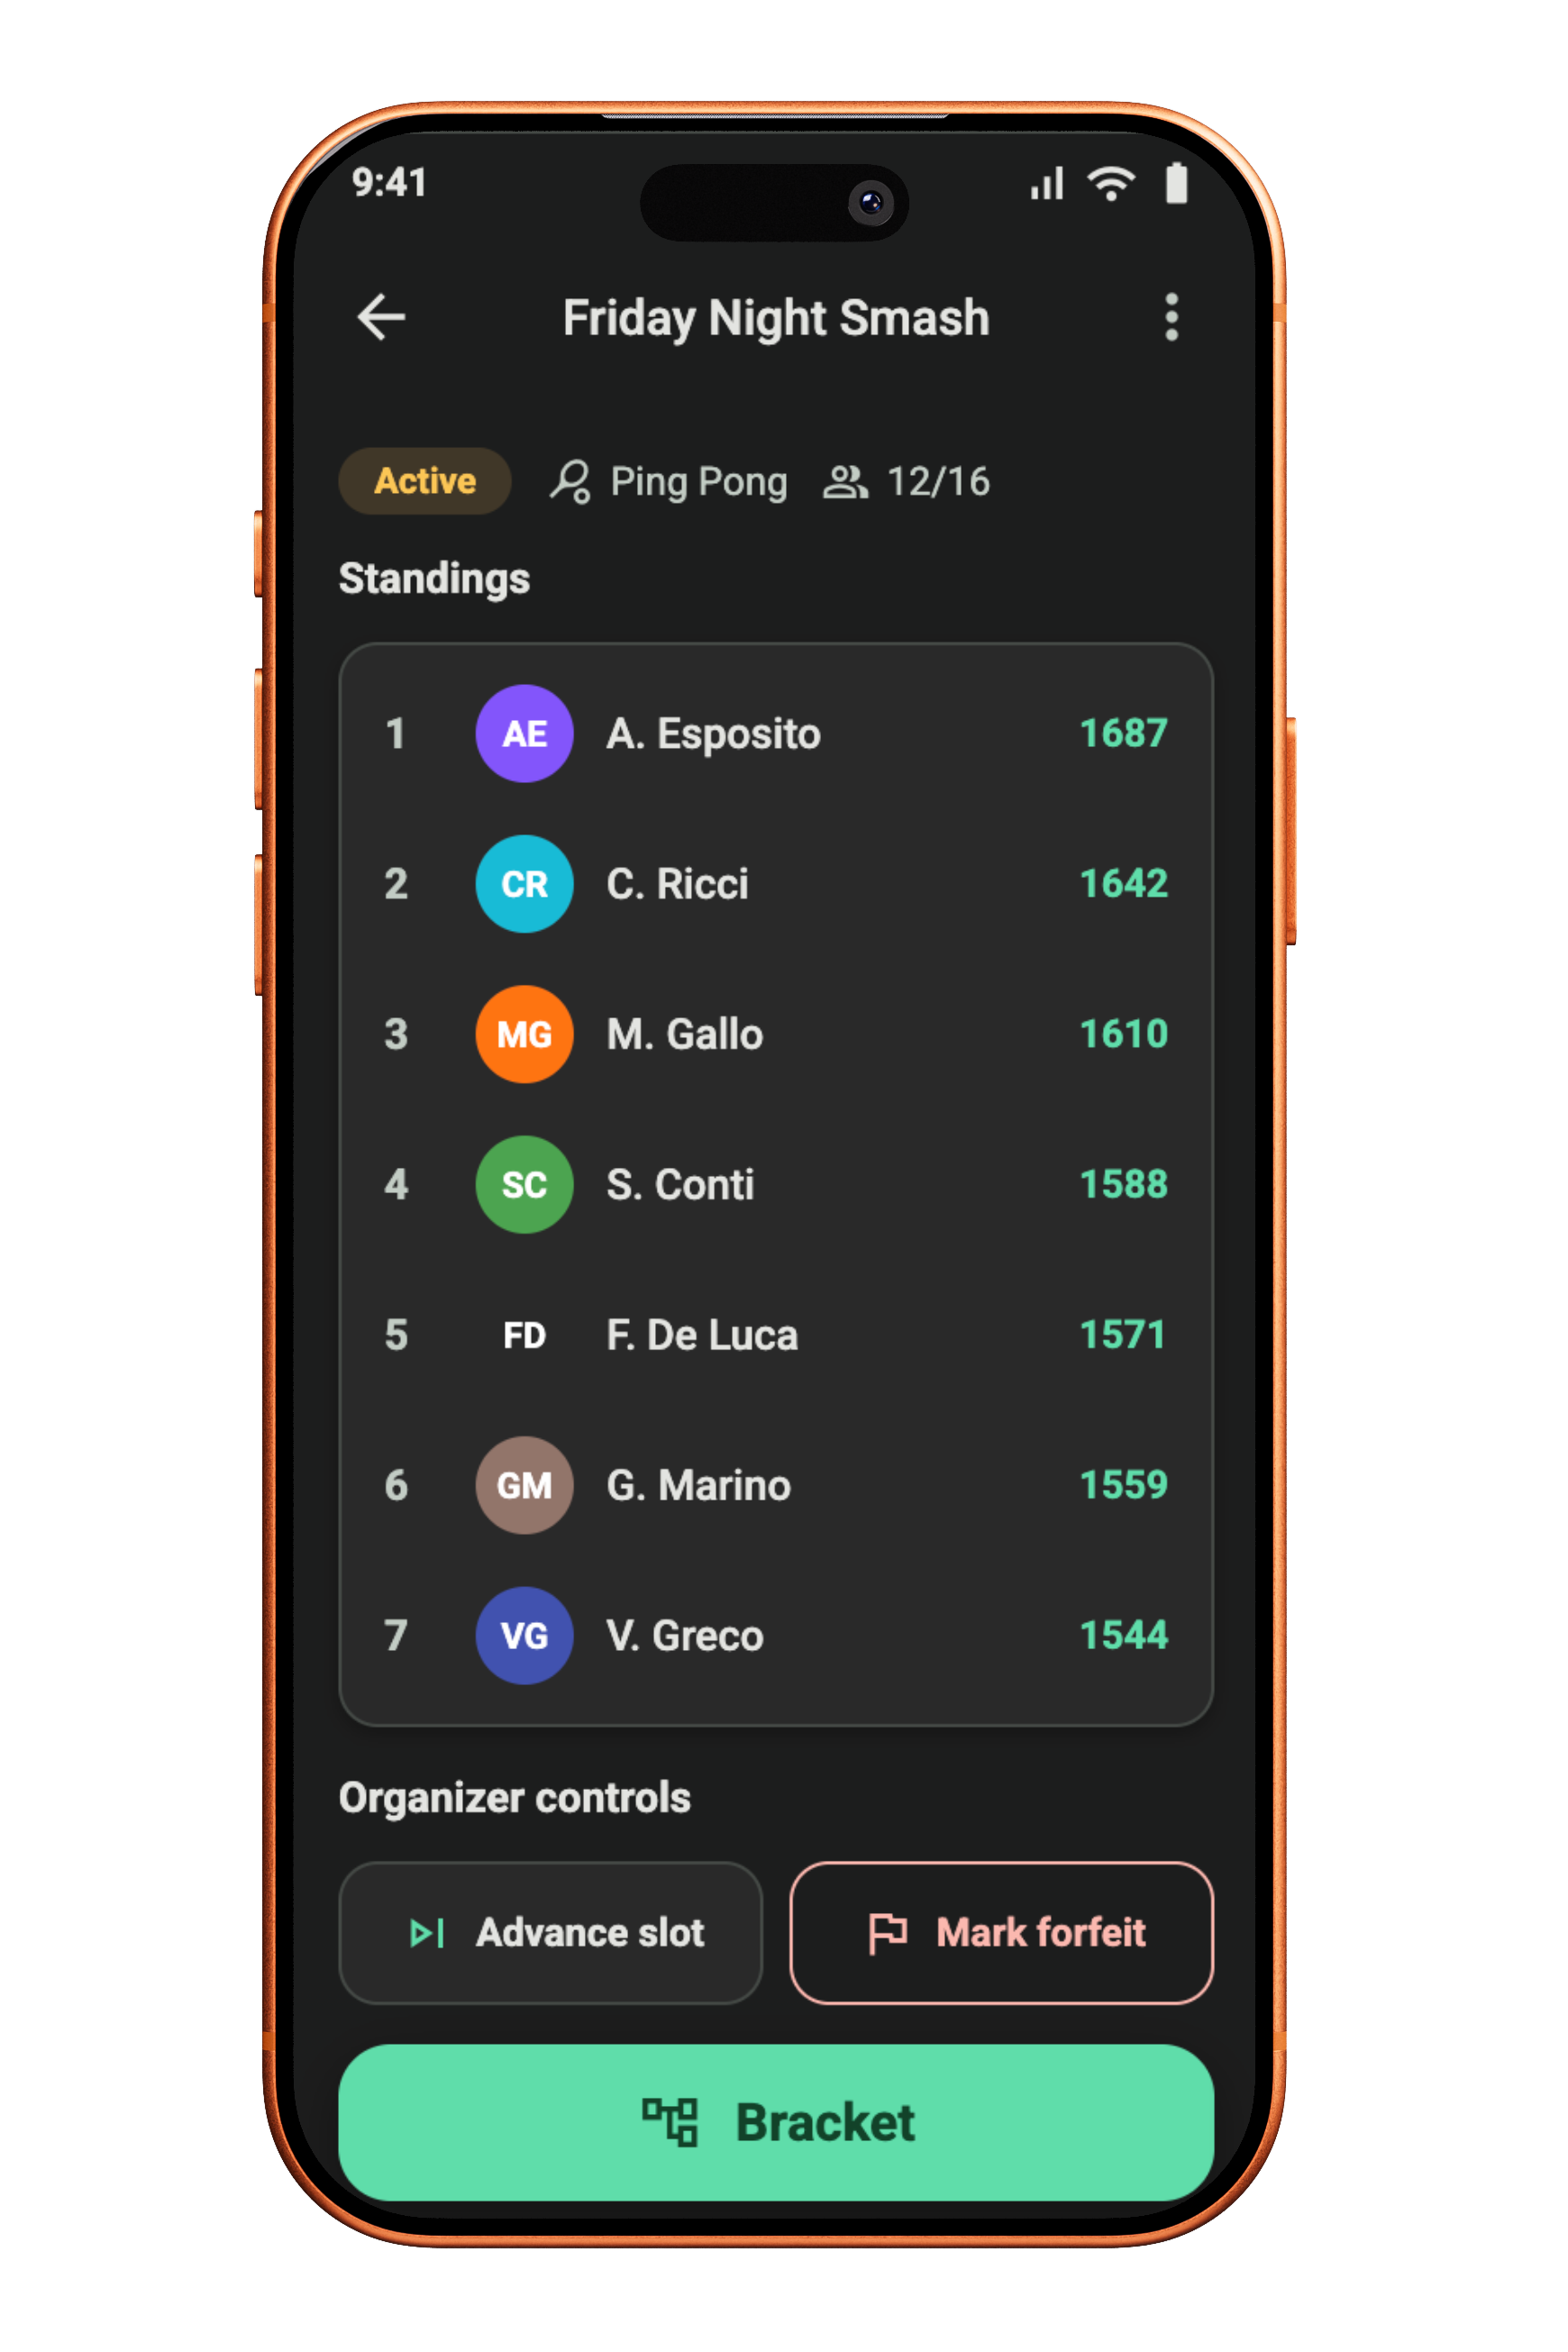
\includegraphics[width=0.25\linewidth]{mockups/standings_en_dark}}
    \caption{Tournament browser, creation form, live single-elimination bracket, and the tournament detail screen with organiser controls.}
    \label{fig:tournament_screens}
\end{figure}

\begin{figure}[H]
    \centering
    \subfloat[Opening state]{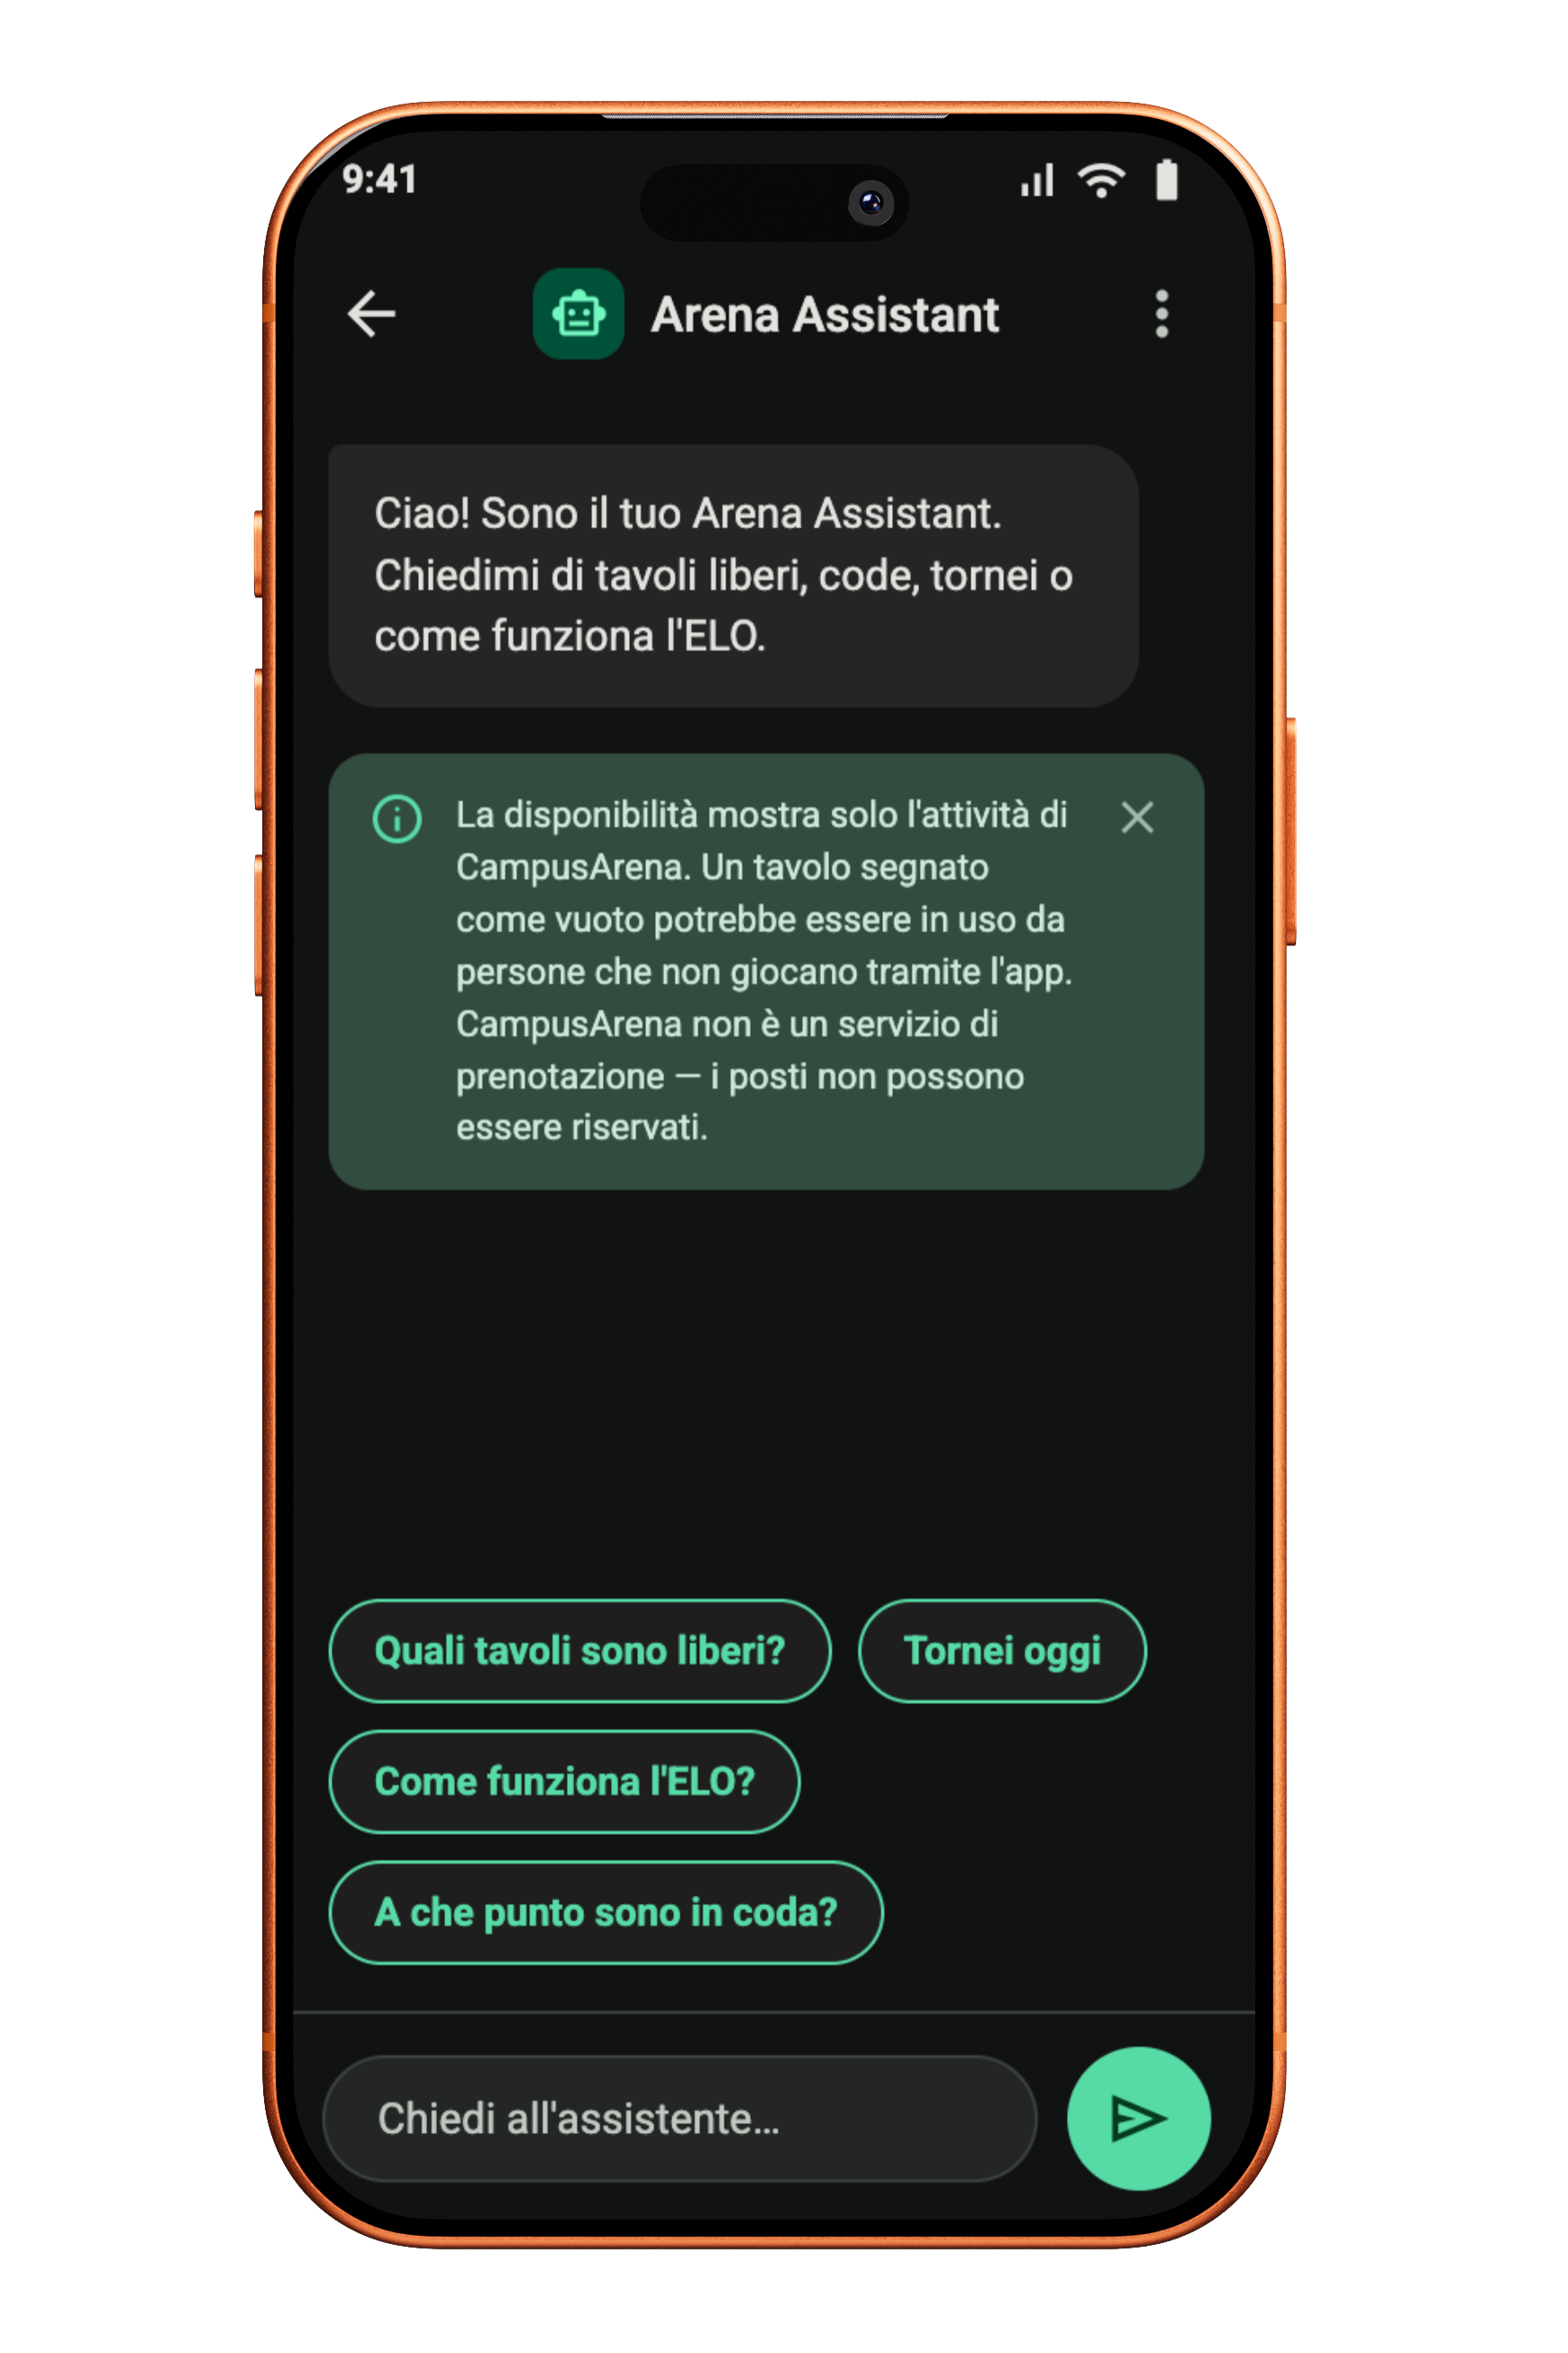
\includegraphics[width=0.3\linewidth]{mockups/assistant_it_dark}}\hfill
    \subfloat[Rich answer card]{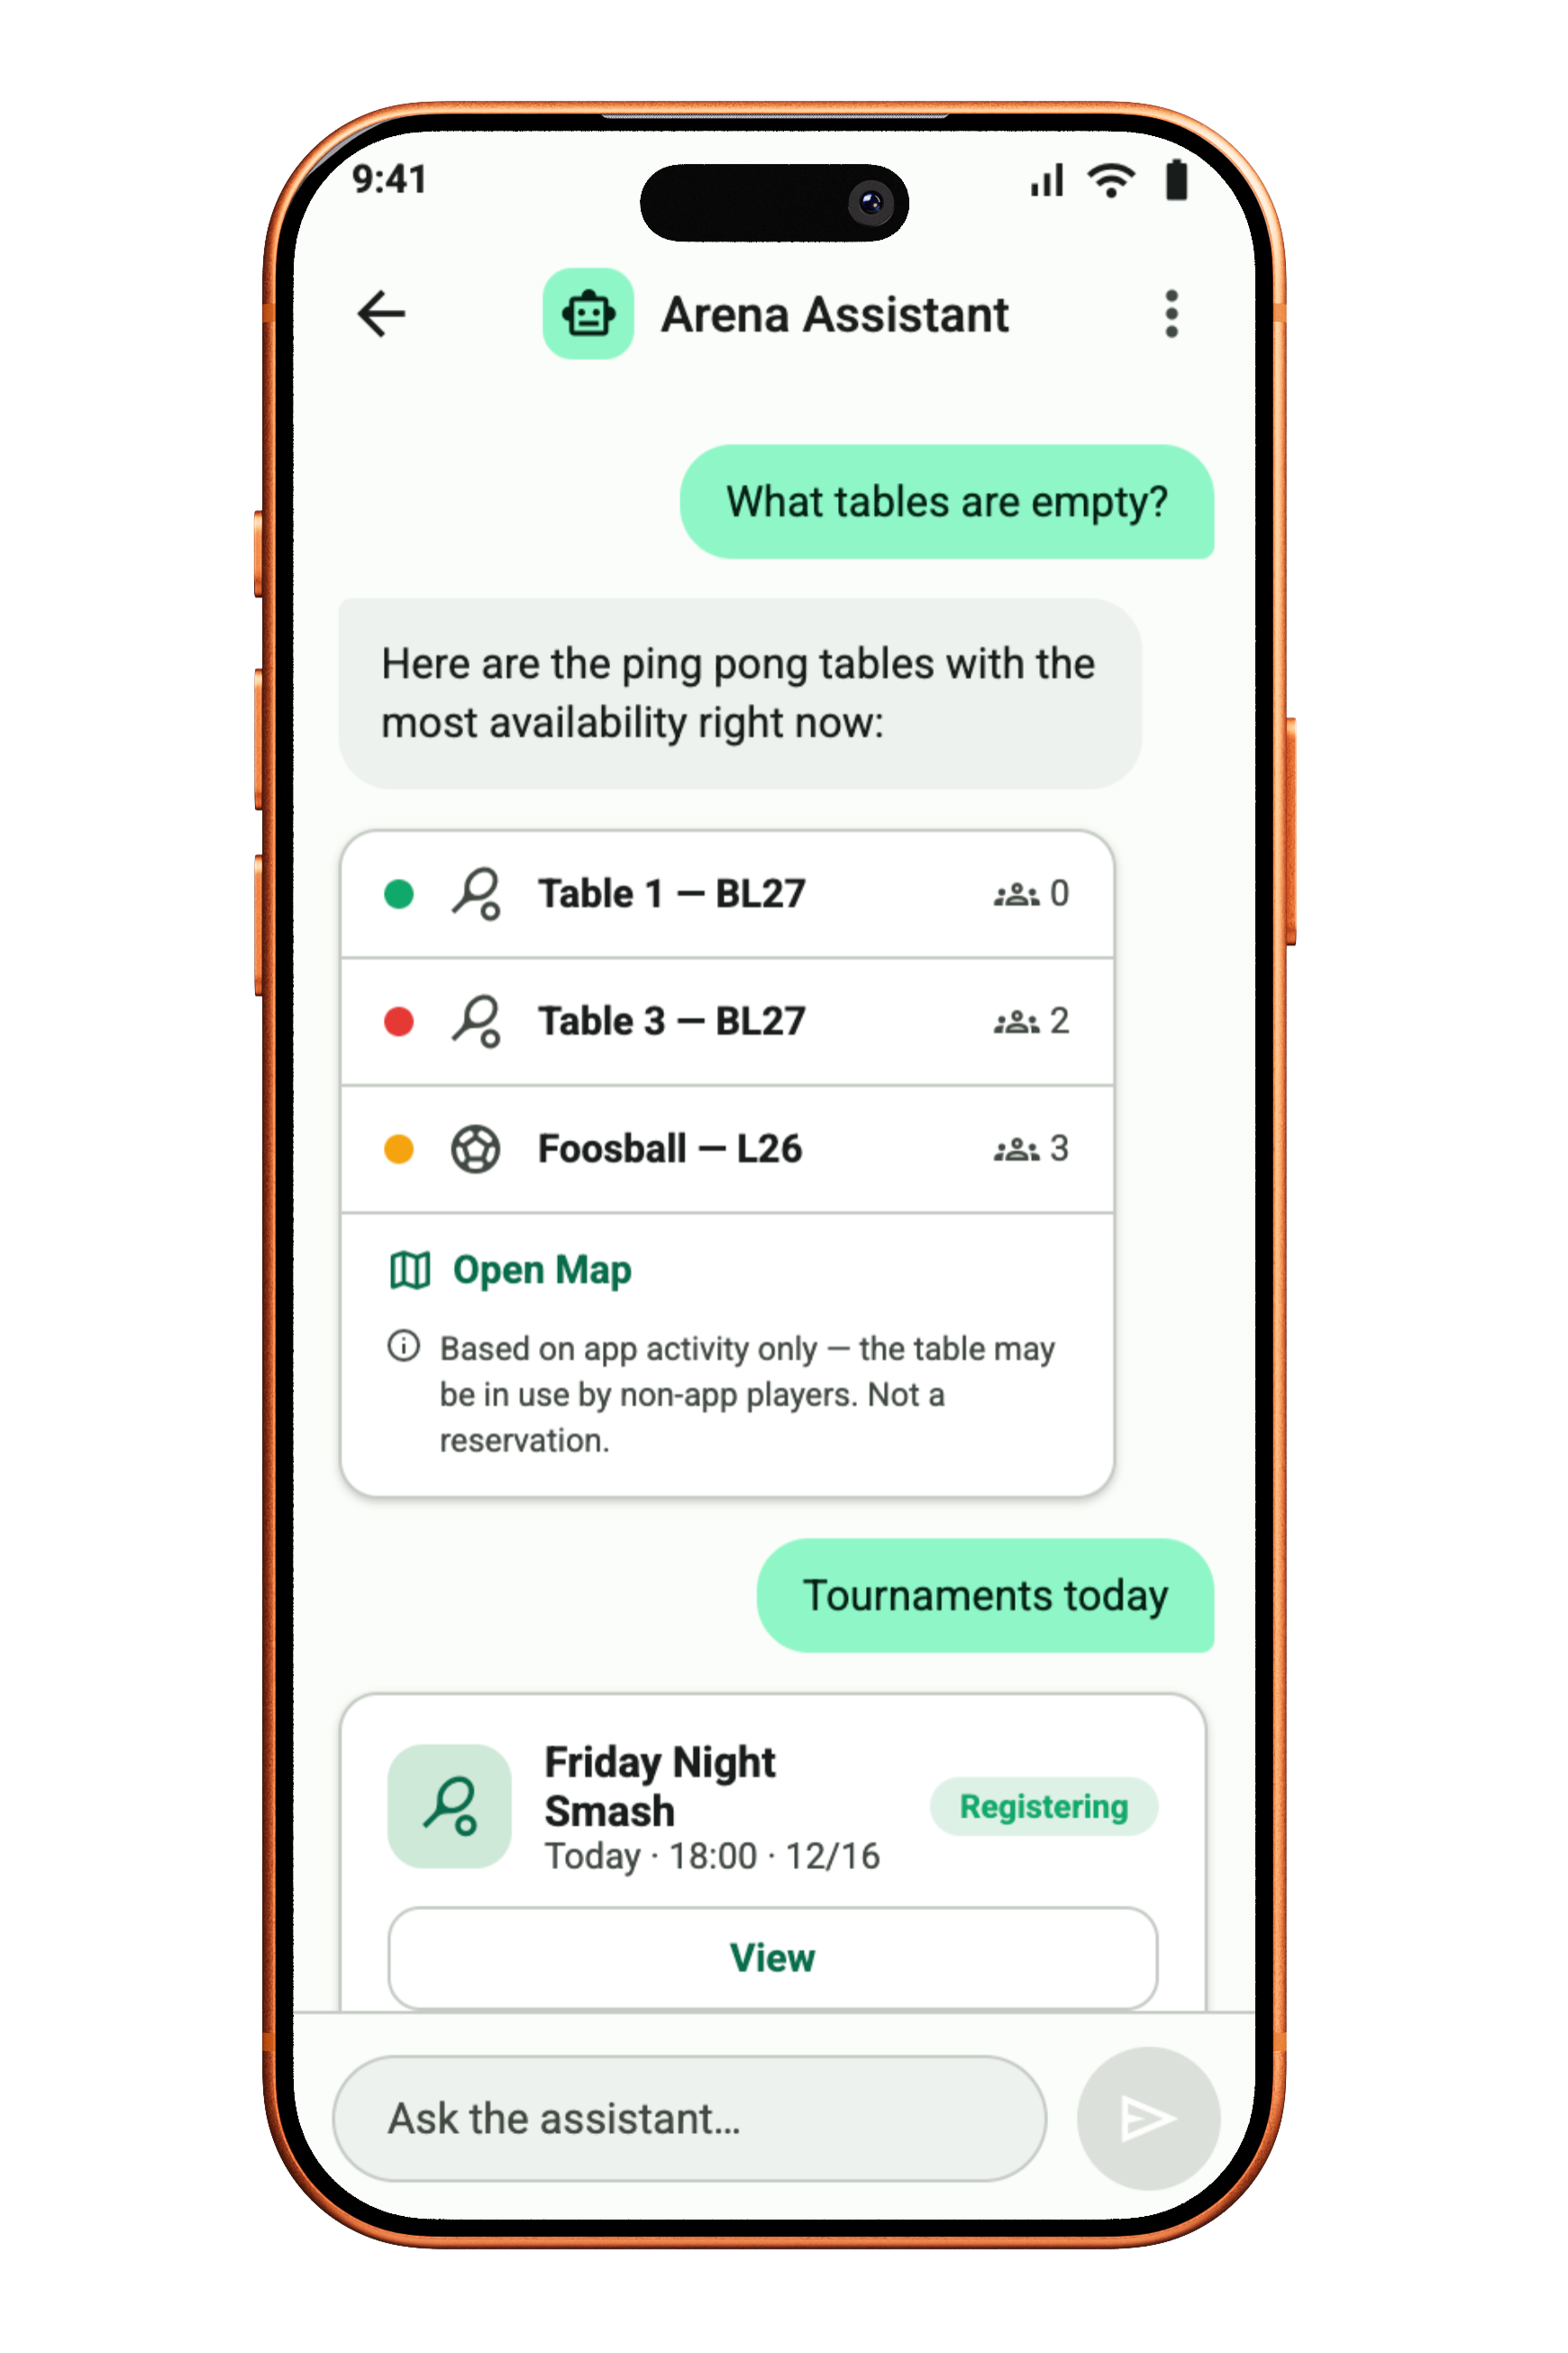
\includegraphics[width=0.3\linewidth]{mockups/assistantrichcard_en_light}}\hfill
    \subfloat[Error / retry]{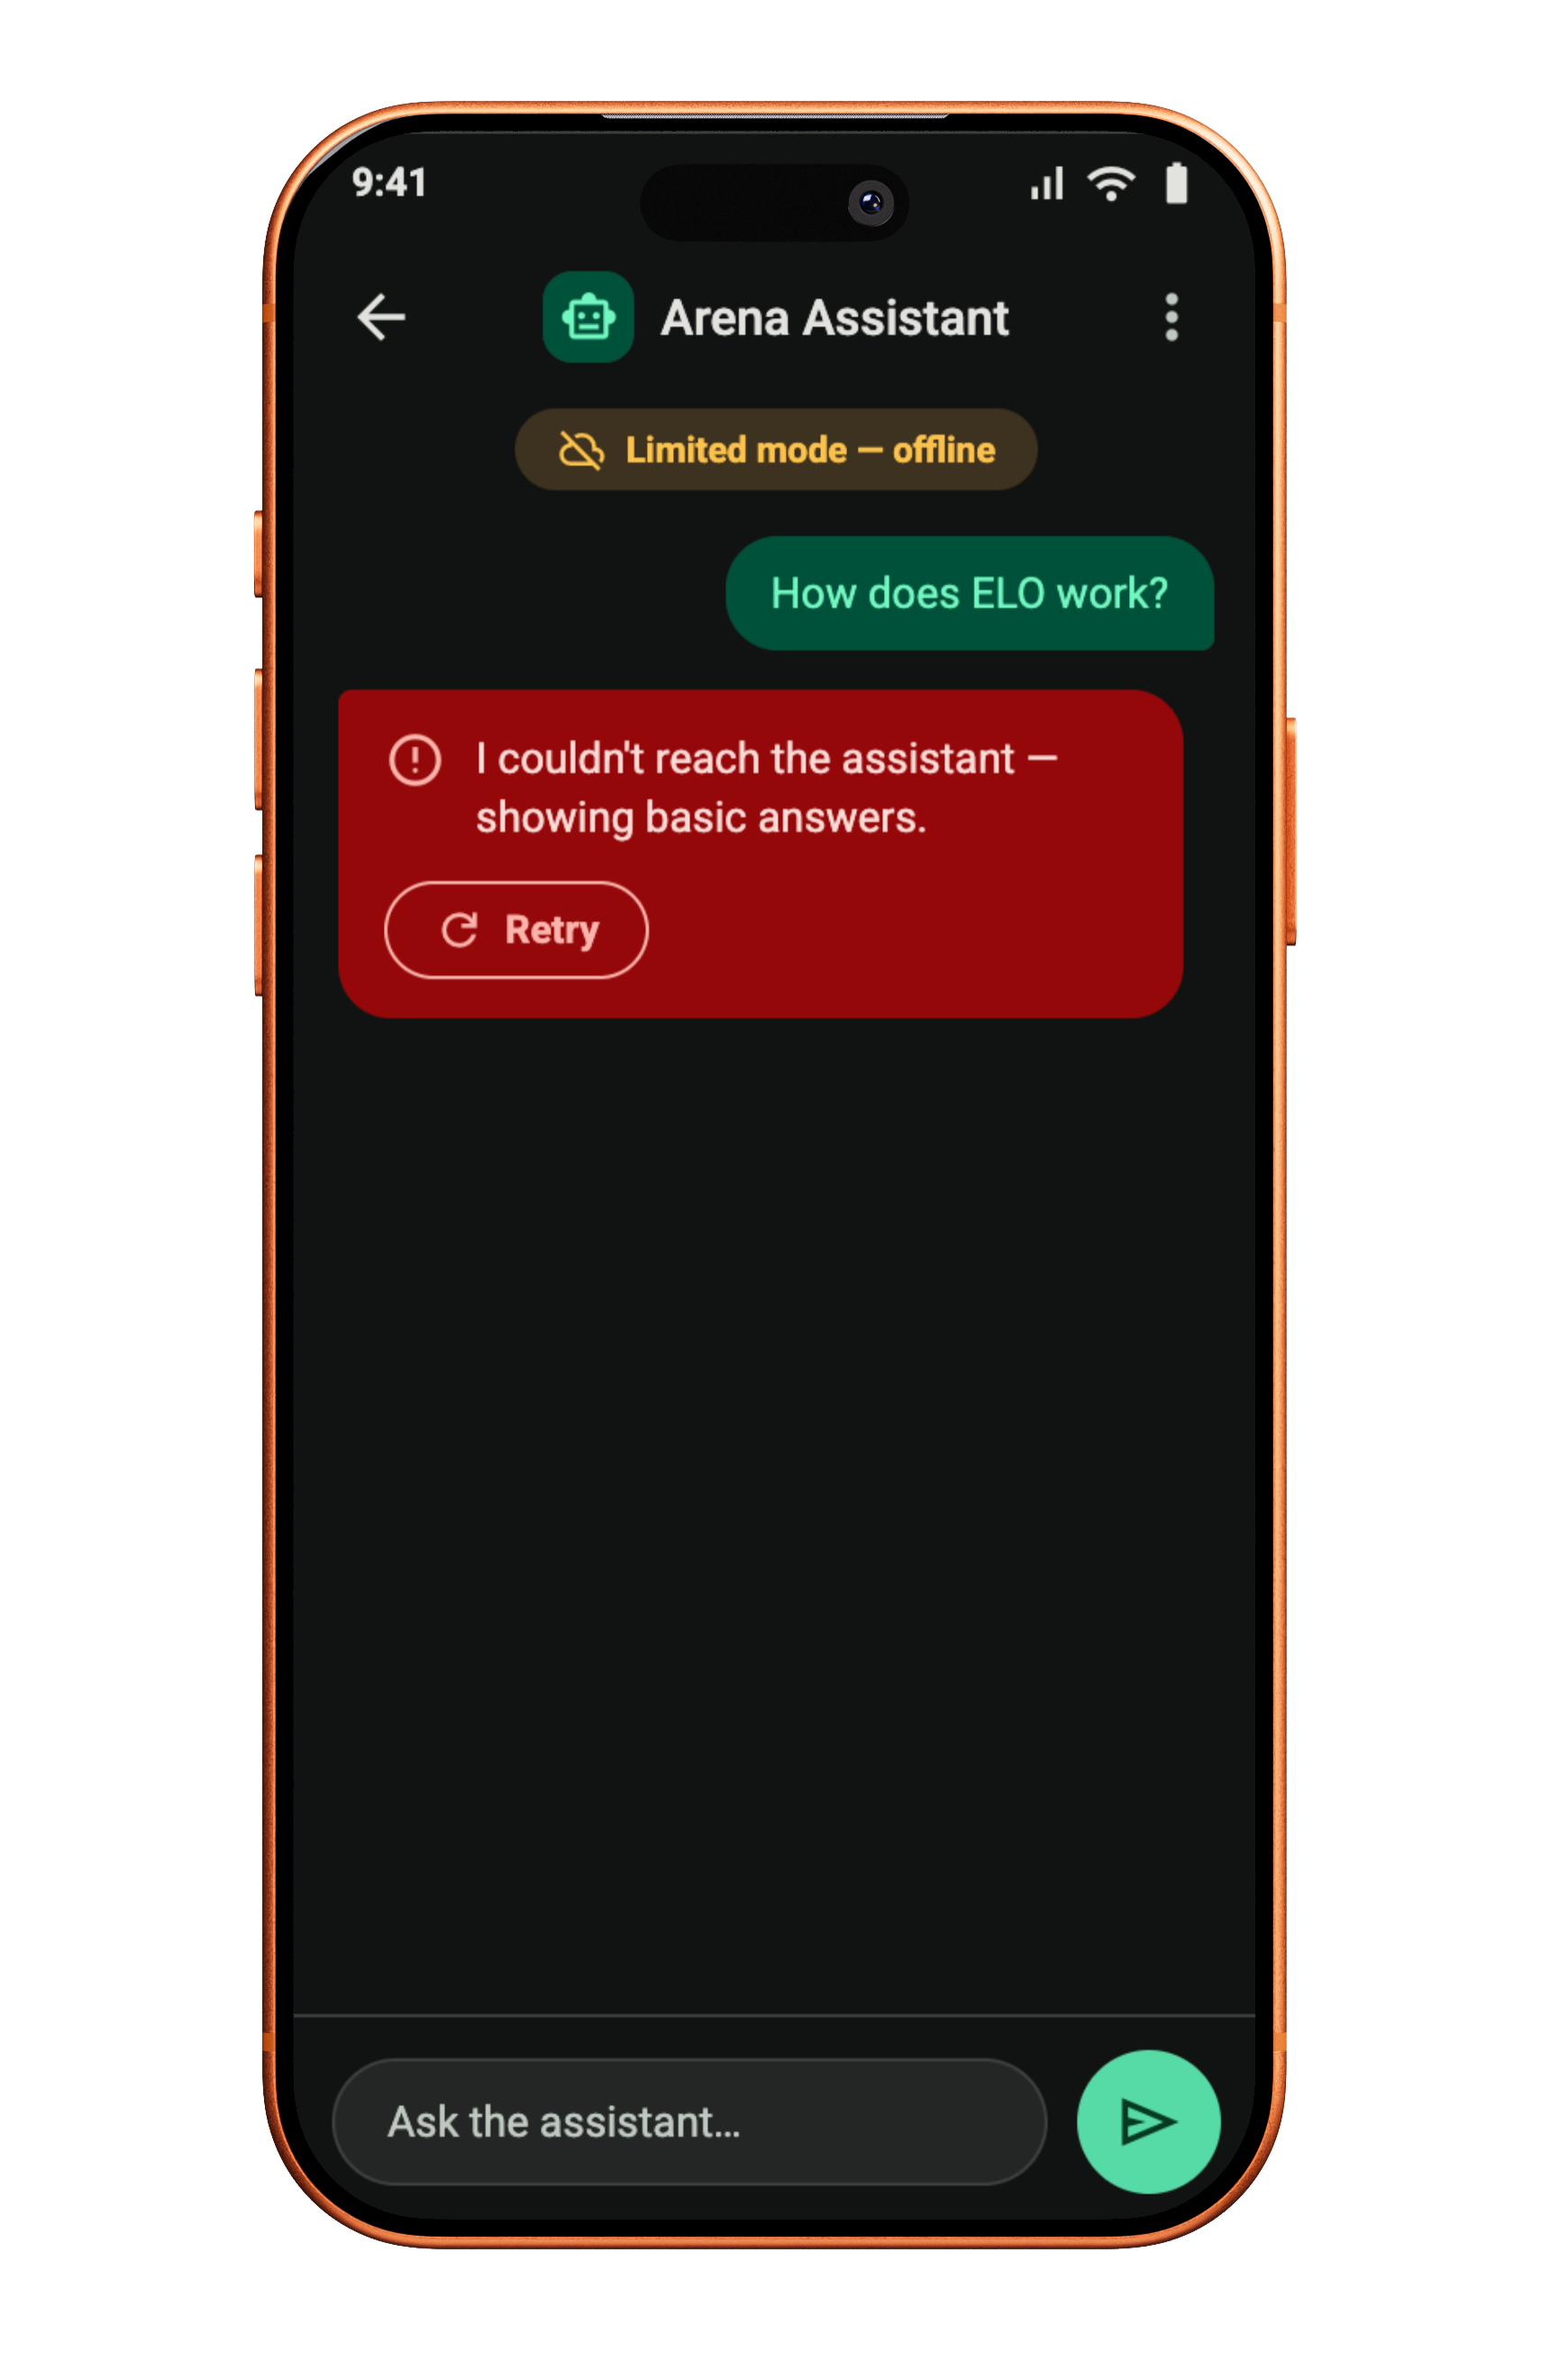
\includegraphics[width=0.3\linewidth]{mockups/assistanterror_en_dark}}
    \caption{Arena Assistant: first-open disclaimer and chips, a grounded answer card, and the error/retry state.}
    \label{fig:assistant_screens}
\end{figure}

\begin{figure}[H]
    \centering
    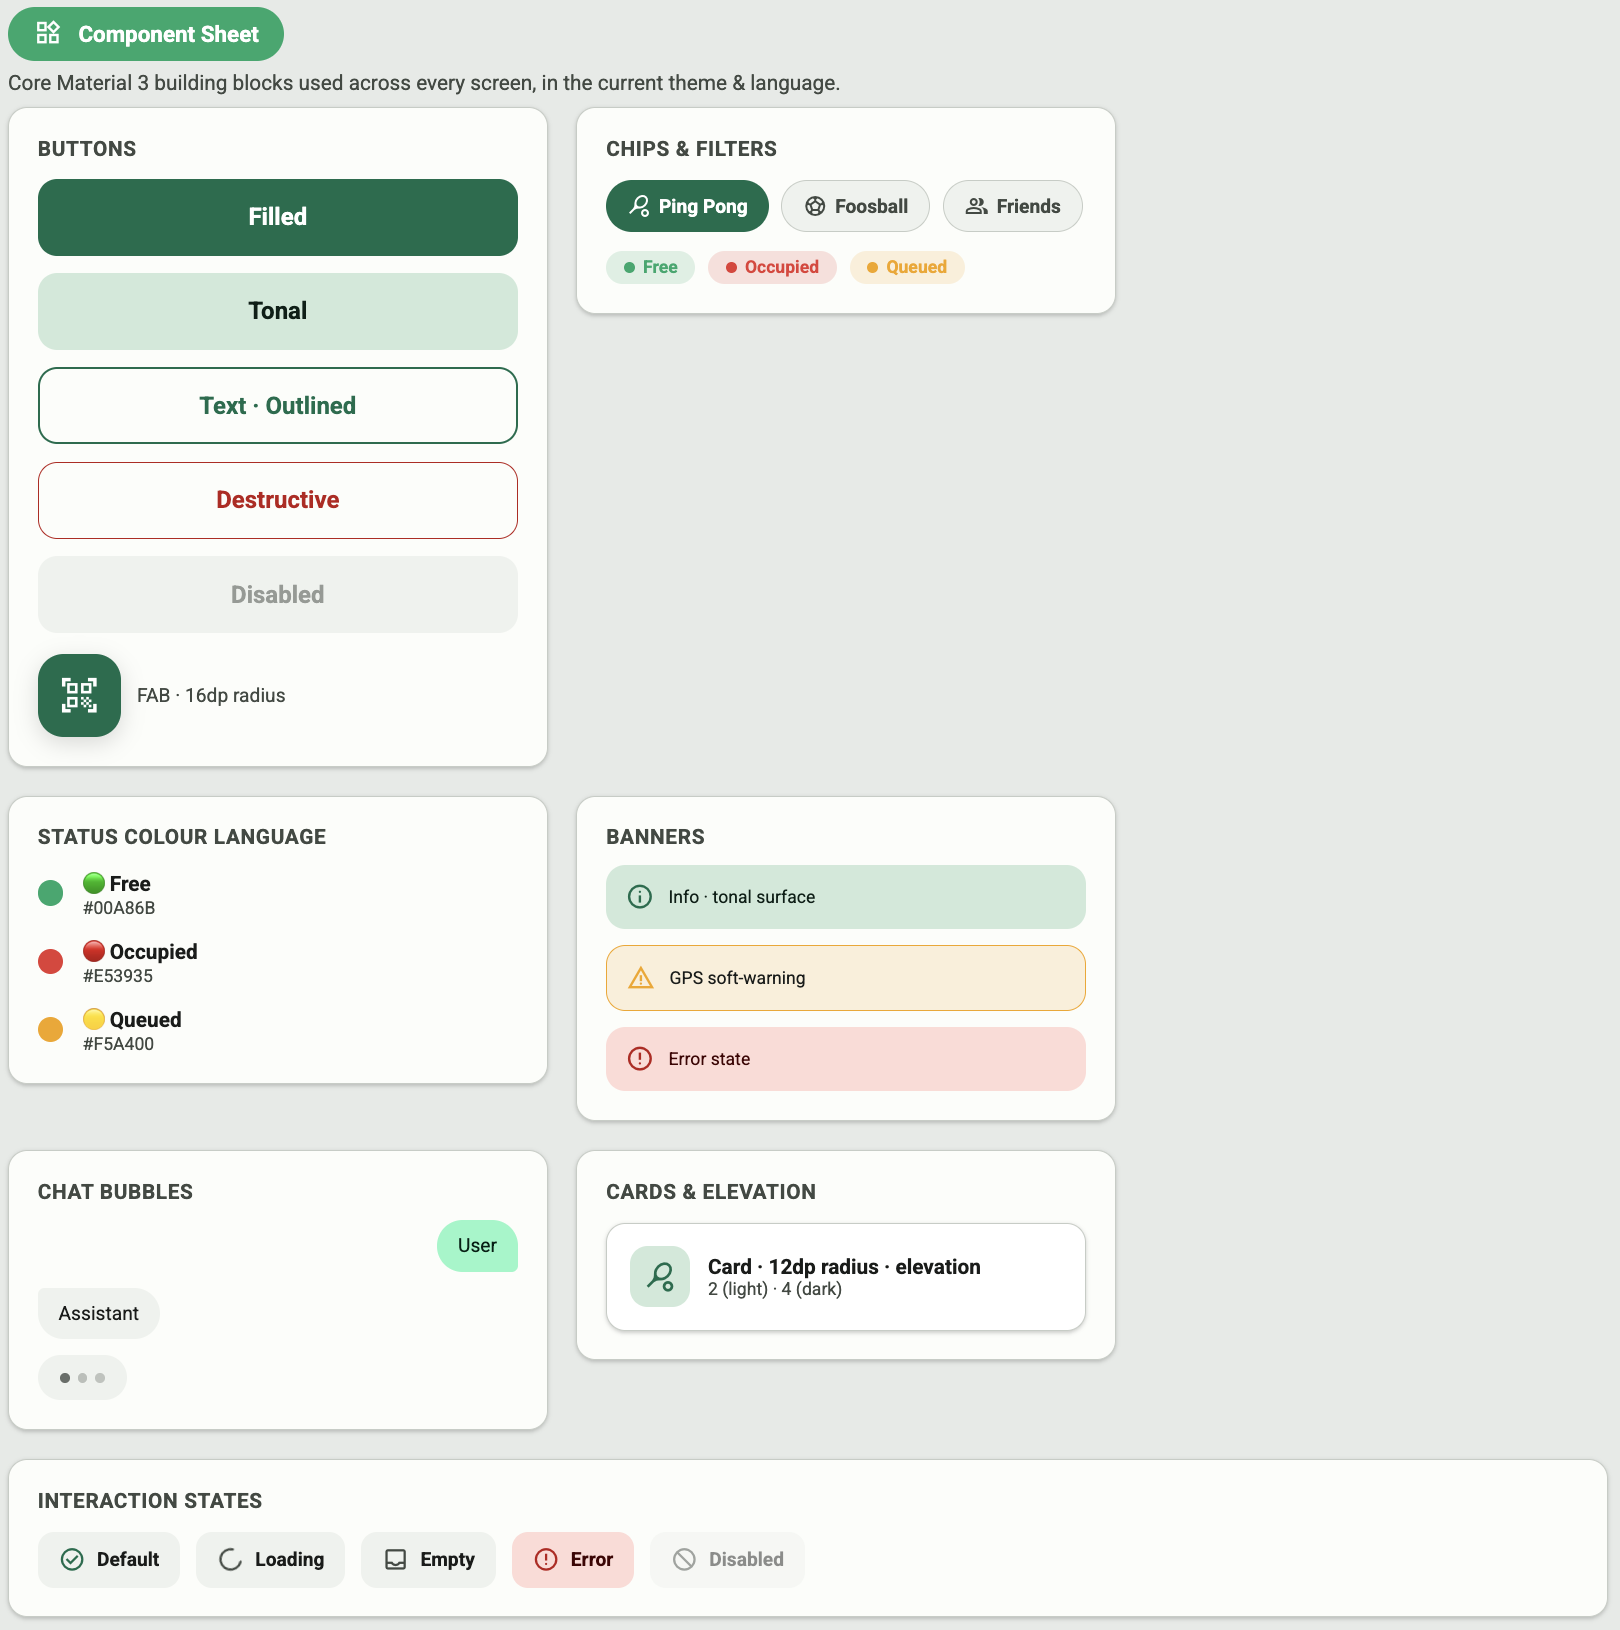
\includegraphics[width=0.5\linewidth]{screenshots/componentsheet_en_light}
    \caption{The design-system component sheet. Every mockup in this catalog alternates deliberately between the light and dark themes and the English and Italian locales, exercising both across the screen set.}
    \label{fig:crosscutting_screens}
\end{figure}

\section{Tablet Adaptivity}
\label{sec:responsive}

Responsiveness follows a single breakpoint used consistently: \textbf{600\,dp} of available width, checked with \texttt{LayoutBuilder} constraints (for the shell) and \texttt{MediaQuery.sizeOf} (for screen-level decisions).

\begin{itemize}
    \item \textbf{Navigation chrome.} Below 600\,dp, \texttt{AppShell} shows a Material 3 \texttt{NavigationBar}; at 600\,dp and above it switches to a \texttt{NavigationRail} with a leading app badge, and the \texttt{MaterialApp.builder} removes the now-unneeded bottom padding so rail layouts run edge to edge.
    \item \textbf{Split views.} The two highest-density screens get true two-pane tablet layouts. The Map shows the interactive map and the facility list side by side, with the detail card docked instead of sliding over. Home shows the ELO hero card and sport selector alongside the activity column, removing the phone's vertical scroll.
    \item \textbf{Everything else} is made correct on a large canvas through constrained, centred content (forms, leaderboards, chat) rather than bespoke layouts, which keeps the widget-test matrix tractable. Both orientations work; nothing is locked to portrait.
\end{itemize}

\begin{figure}[H]
    \centering
    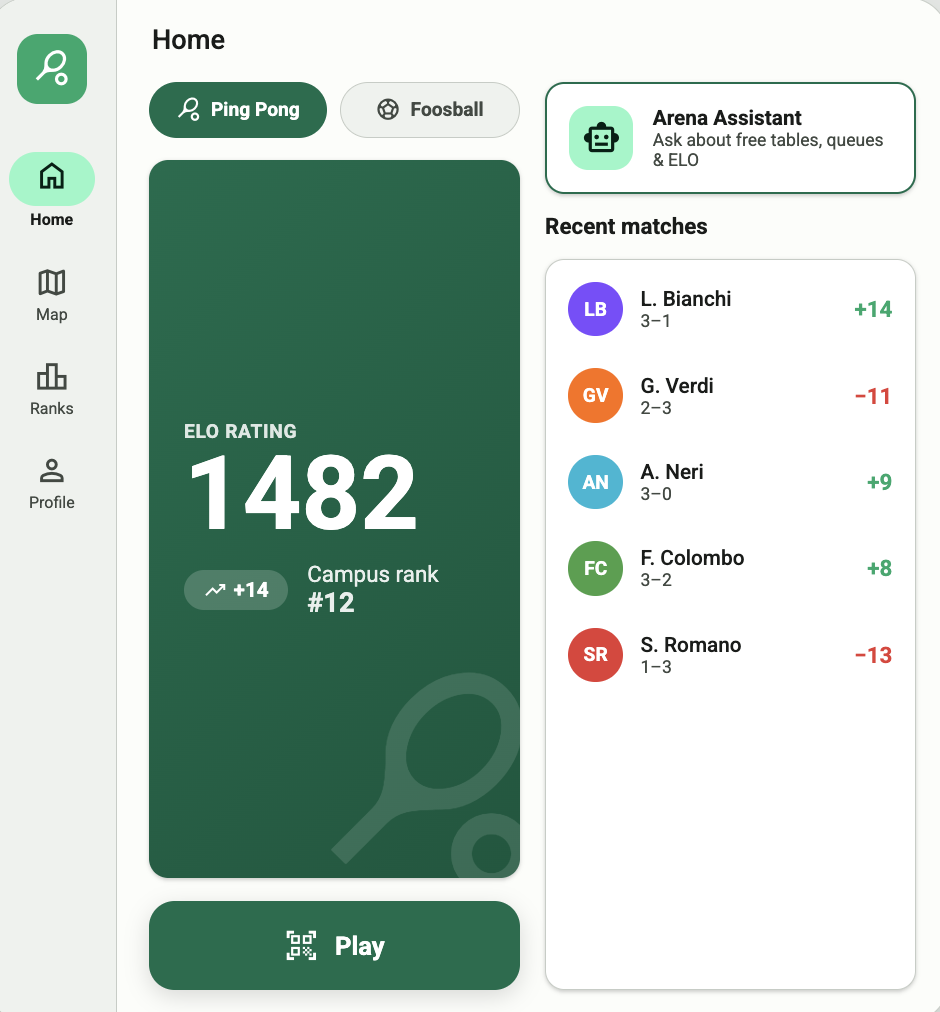
\includegraphics[width=0.5\linewidth]{screenshots/tablet_en_light}
    \caption{The Home dashboard as a bespoke two-pane tablet split-view, with the \texttt{NavigationRail} replacing the phone's bottom \texttt{NavigationBar}.}
    \label{fig:tablet_split}
\end{figure}

\section{Localisation}
\label{sec:localisation}
The app ships in English and Italian through \texttt{flutter\_localizations} and \texttt{intl} with ARB files (\texttt{app\_en.arb}, \texttt{app\_it.arb}, compiled into \texttt{lib/l10n/}). No user-facing string is hardcoded: screens, dialogs, validation errors (including Firebase Auth error mapping), badge names/descriptions (through the \texttt{nameKey}/\texttt{descriptionKey} indirection in \texttt{achievementDefs}), the tutorial, and both chatbot disclaimers are all keyed. Plurals, dates, and numbers go through \texttt{intl} formatting. Player names, usernames, and ELO values are data and are never translated. The language is chosen in Settings, persisted on the user document, and seeded into \texttt{LocaleCubit} at sign-in so a choice follows the user across devices; before sign-in the system locale applies.

\section{Theming and Dark Mode}
\label{sec:theming}
The visual identity is a Material 3 theme generated from a single seed colour, emerald green \texttt{\#00A86B} (\texttt{AppTheme.primarySeedColor}), with \texttt{ColorScheme.fromSeed} producing the light and dark schemes. The dark theme darkens surfaces explicitly (\texttt{\#121212} scaffold, \texttt{\#1E1E1E} cards) for OLED-friendly contrast. \texttt{themeMode} is \texttt{ThemeMode.system}, so the app follows the OS setting and both themes are exercised in testing. Component themes are centralised: 12\,dp corner radii, 48\,dp minimum touch targets, filled text fields with a 2\,dp primary focus border, and a transparent centred app bar. Semantic colours outside the Material scheme — the gold/silver/bronze podium accents — live in a \texttt{PodiumColors} \texttt{ThemeExtension} with separate light and dark palettes, and a fixed avatar palette keeps identity colours stable across themes.

\section{Design System}
\label{sec:design_system}
The mockups in this chapter are sourced from the project's implemented design system, an interactive HTML/CSS catalog of every component and screen across both themes and both locales — rather than a separate design-tool file. Anchoring the mockups to the design system the app is actually built against keeps them executable and drift-free.

% ============================================================
%   CHAPTER 6 — TESTING AND QUALITY ASSURANCE
% ============================================================

\chapter{Testing and Quality Assurance}
\label{ch:testing_quality}

The team planned the testing approach up front, before implementation started, and the final suite follows that plan closely. The \texttt{app/test/} tree mirrors \texttt{app/lib/} and comprises \textbf{105 test files} (plus 3 shared helper files) containing roughly \textbf{864 test-case declarations}. The suite is deterministic by construction: time-dependent logic (decay, penalties, timeouts, queue eviction) always accepts an injected \texttt{now}, and all network and Firebase access is replaced by fakes or mocks.

\section{Test Levels}
\begin{itemize}
    \item \textbf{Unit tests} target pure Dart logic with no framework and no I/O: \texttt{EloCalculator}, the single-elimination bracket builder in \texttt{bracket\_engine.dart}, the \texttt{ScoringStrategy} implementations, \texttt{AchievementEvaluator}, input validators, and all models. They are fast and assert exact values (an equal-rating win at $K=32$ moves exactly 16 points; a 400-point favourite has an expected score of $\approx 0.909$).
    \item \textbf{Repository tests} verify the data layer against \texttt{fake\_cloud\_firestore}, an in-memory Firestore that honours references, queries, and transactions. This level occupies the space integration tests would normally fill: a repository test drives a realistic multi-document flow (create match, submit, confirm, observe ELO writes on two rating documents and a facility flip) entirely in process. All ten repositories have a dedicated file.
    \item \textbf{Cubit tests} verify state management in isolation using \texttt{bloc\_test} and \texttt{mocktail}, stubbing success or failure responses and asserting the exact emitted-state sequences. Every Cubit has a test file.
    \item \textbf{Widget tests} pump screens or components with \texttt{flutter\_test}, backed by mocked repositories or a seeded fake Firestore, verifying rendering, form validation, tap interactions, dialog flows, and localised text in both locales. \textbf{Routing tests} are a specialisation: they mount the real \texttt{createRouter} inside a \texttt{MaterialApp.router} and verify redirect behaviour against a scripted \texttt{AuthCubit}.
    \item \textbf{Cross-vertical integration tests} (\texttt{app/test/integration/}) exercise the three shared contracts on \texttt{fake\_cloud\_firestore}: the match document at confirmation (read by profile/history), the facility status flip (read by the map), and the queue ticket (read by check-in).
\end{itemize}

\section{Frameworks and Test Doubles}
\begin{table}[H]
    \centering
    \small
    \begin{tabularx}{\textwidth}{l l X}
        \textbf{Package} & \textbf{Version} & \textbf{Role} \\\hline\\[-9px]
        \texttt{flutter\_test} & SDK & Test runner, \texttt{testWidgets}, finders, matchers, \texttt{WidgetTester}. \\[3px]
        \texttt{bloc\_test} & 10.0.0 & Declarative Cubit tests: \texttt{build}/\texttt{act}/\texttt{expect}/\texttt{verify}, error injection. \\[3px]
        \texttt{mocktail} & 1.0.5 & Null-safe mocks without code generation; stubbing repositories and Firebase types. \\[3px]
        \texttt{fake\_cloud\_firestore} & 4.1.1 & In-memory Firestore: collections, queries, snapshots, transactions. \\[3px]
        \texttt{flutter\_lints} & 6.0.0 & Static-analysis rule set enforced by CI alongside the tests. \\[3px]
    \end{tabularx}
    \caption{Testing frameworks and tools.}
    \label{tab:test_frameworks}
\end{table}

The suite uses two families of doubles, chosen by layer. At the \textbf{repository level} the double is a \emph{fake}: \texttt{FakeFirebaseFirestore} is seeded through the production model classes (\texttt{toMap}) and read back through \texttt{fromMap}, so serialisation is exercised on both sides and tests verify actual query semantics and transaction atomicity. At the \textbf{Cubit and widget level} repositories are replaced with \texttt{mocktail} mocks, and stream APIs are stubbed with \texttt{StreamController}s so tests can push auth or snapshot updates at controlled moments. Three shared helpers keep this consistent: \texttt{auth\_test\_helpers.dart} (authenticated/unauthenticated \texttt{AuthCubit} factories), \texttt{fake\_tile\_provider.dart} (a synthetic \texttt{flutter\_map} tile provider so map tests never hit OSM), and \texttt{queue\_test\_helpers.dart} (queue/facility seeding).

\section{Test Inventory}
\begin{table}[H]
    \centering
    \small
    \begin{tabularx}{\textwidth}{l r X}
        \textbf{Module} & \textbf{Files} & \textbf{Focus} \\\hline\\[-9px]
        \texttt{test/core/} & 10 & ELO calculator, scoring strategies, bracket engine, achievement evaluator, validators, map defaults. \\[3px]
        \texttt{test/models/} & 7 & Model serialization round-trips and \texttt{copyWith}. \\[3px]
        \texttt{test/repositories/} & 10 & All repositories against \texttt{fake\_cloud\_firestore}, including every transactional path. \\[3px]
        \texttt{test/features/} & 70 & Cubit transitions (\texttt{bloc\_test}) and screen/widget tests per feature, both locales. \\[3px]
        \texttt{test/routing/} & 3 & Shell tab navigation and public-profile drill-in; registration and auth-redirect edge cases. \\[3px]
        \texttt{test/integration/} & 3 & The three cross-vertical shared contracts. \\[3px]
        \texttt{test/l10n/} & 1 & Both-locale render check. \\[3px]
        \texttt{test/widget\_test.dart} & 1 & Application smoke test: full app boot to an authenticated home screen. \\[3px]
        \textbf{Total} & \textbf{105} & $\approx$864 test-case declarations. \\[3px]
    \end{tabularx}
    \caption{Automated test inventory by module.}
    \label{tab:test_inventory}
\end{table}

\section{Notable Test Cases}
The following clusters verify the most failure-prone behaviour in the system.

\begin{itemize}
    \item \textbf{K-factor boundary.} \texttt{kFactor(9)} returns 32 and \texttt{kFactor(10)} returns 16; because \texttt{matchesPlayed} is the pre-match count, a player with 9 recorded matches is playing their tenth and is still rated at $K=32$ (delta of exactly 16 on an even win). Re-verified through the persistence layer.
    \item \textbf{Lazy inactivity decay.} No decay within the 30-day grace period; exactly one point per whole idle day afterwards; partial days ignored; a hard floor at 1200; ratings at or below 1200 untouched. Repeated reads at the same instant never compound, and a repository case proves the decayed value becomes \texttt{eloBefore}.
    \item \textbf{One canonical pair identity.} \texttt{pairIdFromUids} sorts UIDs, is order-independent, and does not mutate input; a decisive case asserts \texttt{pairIdFromUids(uids) == RatingRepository.pairId(uids)}, enforcing one implementation shared by calculator and repository.
    \item \textbf{Bracket byes and TBD.} The number of first-round byes equals \texttt{bracketSize - N} for 5, 6, 7 participants; a bye slot is not playable and reports the real player as winner; an unresolved feeder yields a \texttt{TBD} slot (not a bye), so a waiting player never appears to advance for free.
    \item \textbf{Forfeit advancement without double-counting.} A mid-bracket forfeit advances the opponent and makes the final playable; a player who is both eliminated and the confirmed loser is resolved by the match, so the forfeit branch does not fire twice.
    \item \textbf{The confirm transaction moves together or not at all.} From a single \texttt{confirmResult} call: the match becomes \texttt{confirmed} with \texttt{eloBefore}/\texttt{eloDeltas} snapshotted (\texttt{\{u1: 16, u2: -16\}}), both ratings move to 1216/1184 with incremented counts, and the facility returns to \texttt{free}. The doubles variant proves the \emph{pair} entity is rated (keys \texttt{u1\_u2}, \texttt{u3\_u4}) while all four singles ratings stay untouched. Guard cases assert \texttt{StateError} outside the valid state.
    \item \textbf{Dispute escalation and penalty interception.} A first/second dispute frees the facility, writes no ELO, and increments the counter; the third resets it and writes a 7-day penalty; a penalised dispute is force-confirmed with real ELO (deltas $\pm 16$), not a punitive fallback. \texttt{now} is injected for determinism.
    \item \textbf{Queue eviction on claim.} Front-runners are purged when the table freed $>5$ minutes ago and preserved when recent; the scanner's own ticket is always deleted; a scanner at position 2 purges the no-show at position 1 while position 3 survives, leaving the facility correctly queued for them.
    \item \textbf{Scoring-strategy validation.} Ping-pong legal results (best-of-3, a 12--10 deuce set, a 21-point game) and typed rejections (\texttt{setNotDecisive}, \texttt{tiedSet}, \texttt{malformedResult}, \texttt{winnerMismatch}); foosball repeats the pattern; the factory resolves each sport id to the right strategy.
    \item \textbf{Registration failure must not bounce off the form.} A regression test (from a review blocker): \texttt{signUp} succeeds and the auth stream reports a user, which would unmount \texttt{RegisterScreen} before \texttt{createUser} rejects a taken username. The test drives the real router and asserts the screen stays mounted with the ``username already taken'' \texttt{SnackBar}, including the orphaned-account cleanup path.
    \item \textbf{Authenticated shell navigation.} The production router boots to \texttt{HomeScreen}; each \texttt{NavigationBar} destination renders its screen; and \texttt{publicProfile('other-uid')} reuses \texttt{ProfileScreen} for a foreign user while hiding the settings gear.
    \item \textbf{The disclaimer is enforced in code.} The availability disclaimer is present on the rule-based path with no key, present on the LLM path even when the mocked response omits it, and absent when no availability tool fired.
\end{itemize}

\section{Continuous Integration}
Automated verification runs on GitHub Actions (\texttt{.github/workflows/flutter\_ci.yml}) on every push and pull request to \texttt{main}/\texttt{develop}. A single job on \texttt{ubuntu-latest} (working directory \texttt{./app}) runs: checkout; Flutter setup (stable, cached); \texttt{flutter pub get}; \texttt{dart format -{}-set-exit-if-changed .}; \texttt{flutter analyze -{}-fatal-infos -{}-fatal-warnings} (a binary gate under \texttt{flutter\_lints} plus the project's \texttt{analysis\_options.yaml}); and \texttt{flutter test -{}-coverage}, which produces \texttt{app/coverage/lcov.info}. Generated files (l10n tables, \texttt{firebase\_options.dart}) are filtered out of coverage with \texttt{lcov}, a coverage summary is written to the run, and a human-readable report is posted to the pull request. Branch protection blocks direct pushes to \texttt{main}/\texttt{develop}, requires the CI check to pass, and requires one teammate approval, with feature/fix branches cut from \texttt{develop}.

\section{Test Results}
The final recorded verification run (\texttt{verify\_log.txt}) executed \texttt{flutter pub get}, \texttt{flutter analyze}, and \texttt{flutter test} on a clean checkout: the analyzer reported \emph{No issues found} under the CI configuration that treats infos and warnings as fatal. The full suite runs on every push and pull request through the CI pipeline, and branch protection guarantees that the state of \texttt{develop} and \texttt{main} at submission time corresponds to a fully green suite. Reported case counts are conservative lower bounds on executed assertions, because several widget tests loop over layout and locale variants from a single declaration.

\section{Known Limitations and Future Testing Work}
\begin{itemize}
    \item \textbf{No on-device integration tests.} There is no \texttt{integration\_test/} directory; platform-channel behaviour (the camera-driven QR scanner, push delivery, true multi-device sync latency) sits outside the automated suite and was covered by manual exploratory testing on phone and tablet emulators. The natural next step is an \texttt{integration\_test/} suite against the Firebase emulator, starting with the Proof-of-Play flow and the two flagship assistant queries. Running it in CI would add an emulator step to the workflow.
    \item \textbf{No golden tests.} Widget tests assert structure and behaviour, not pixels. A small set of golden files for the bracket at 4/5/8 participants, the achievement grid, and the dashboard at phone/tablet widths would catch visual regressions cheaply.
    \item \textbf{Firestore Security Rules are not covered by automated tests.} The project ships \texttt{firestore.rules} and \texttt{fake\_firebase\_security\_rules} is present transitively, but no test loads the rules into the fake; they were validated manually against the emulator. A \texttt{test/security/} suite that asserts, e.g., a user cannot write another user's rating or confirm a match they did not play, is the highest-value item on this list.
    \item \textbf{Coverage is reported, not gated.} CI uploads \texttt{lcov.info} but no minimum threshold fails the build. Adding a threshold check or a coverage-diff bot would prevent silent erosion.
\end{itemize}

Every business rule the design commits to, from the K-factor boundary to the dispute-penalty ladder, is pinned by at least one automated test with exact expected values, and no code reaches an integration branch without the entire suite passing.

% ============================================================
%   CHAPTER 7 — CONCLUSIONS
% ============================================================

\chapter{Conclusions}
\label{ch:conclusions}

\section{Implementation and Integration Approach}
Development proceeded in vertical slices, so a demonstrable build existed at every point. The foundation (scaffold, theme, localisation wiring, Firebase setup, responsive shell, all models and repositories with tests) came first; then the auth slice replaced the router's placeholder flag with the real \texttt{authStateChanges} guard; then the core loop was integrated end to end (map, facility detail, QR check-in, active match, scoring, confirmation, ELO, leaderboard and profile); breadth followed (queue, weather, charts with the isolate, friends, challenges); tournaments, brackets, and the Arena Assistant landed next; the localisation audit, test completion, and demo seeding were the closing activities. Integration between the three verticals was managed through the shared Firestore data contract: the three shared document surfaces (match at confirmation, facility status flip, queue ticket) were fixed before coding began, which let the verticals develop in parallel without integration drift.

\section{Final Considerations}
CampusArena delivers a complete, multi-sport competitive platform on a responsive Material~3 shell in English and Italian. Modularity is achieved by separating the sport-agnostic Core from per-sport scoring strategies, keeping the system extensible through a single abstraction. Integrity rests on QR-based Proof of Play and dual result confirmation, with GPS captured as a soft audit signal and every competitive write performed inside a Firestore transaction. The Spark-tier constraints were met with informed, documented compromises rather than compromises of the integrity model — being denied Cloud Functions forced a careful account of atomicity and of who runs each piece of logic, and the resulting design has fewer moving parts than a server-triggered one.

\section{Future Work}
Additional sports enabled by the existing \texttt{ScoringStrategy} abstraction (Padel is already a defined sport id awaiting its strategy; 3v3 Basketball would first need the match model's singles/doubles mode split extended to a third, larger squad size), round-robin tournament formats, facility booking, cross-sport affinity matchmaking, a Blaze-tier server for targeted push and server-authoritative side effects (and for full server-side validation of result transitions), on-device integration tests, golden tests, Security-Rules tests, and a web-based administration dashboard.

% ============================================================
%   CHAPTER 8 — REFERENCES
% ============================================================

\chapter{References}
\label{ch:references}

\section{References}
\label{sec:references}

\begin{itemize}
    \item ISO/IEC/IEEE 29148:2018 — \textit{Systems and software engineering — Life cycle processes — Requirements engineering}. ISO/IEC/IEEE, 2018.
    \item The Requirement Engineering and Design Project specification document, A.Y. 2025--2026. Politecnico di Milano.
    \item Arpad E. Elo. \textit{The Rating of Chessplayers, Past and Present}. Arco Publishing, 1978.
    \item Flutter Team. \textit{Flutter Documentation}. \url{https://docs.flutter.dev}. Accessed July 2026.
    \item Felix Angelov et al. \textit{flutter\_bloc — State Management Library}. \url{https://bloclibrary.dev}. Accessed July 2026.
    \item Flutter Team. \textit{go\_router (17.3.0)}. \url{https://pub.dev/packages/go_router}. Accessed July 2026.
    \item Google LLC. \textit{Firebase Documentation — Auth, Cloud Firestore, Cloud Messaging}. \url{https://firebase.google.com/docs}. Accessed July 2026.
    \item \textit{flutter\_map (8.3.1)} and the \textit{OpenStreetMap Tile Usage Policy}. \url{https://operations.osmfoundation.org/policies/tiles/}. Accessed July 2026.
    \item Open-Meteo. \textit{Free Weather API — Documentation}. \url{https://open-meteo.com/en/docs}. Accessed July 2026.
    \item \textit{mobile\_scanner (7.2.0)}. \url{https://pub.dev/packages/mobile_scanner}. Accessed July 2026.
    \item \textit{geolocator (14.0.3)}. \url{https://pub.dev/packages/geolocator}. Accessed July 2026.
    \item \textit{fl\_chart (1.2.0)}. \url{https://pub.dev/packages/fl_chart}. Accessed July 2026.
    \item Regolo AI. \textit{EU-hosted LLM Inference Platform}. \url{https://regolo.ai}. Accessed July 2026.
    \item \textit{bloc\_test}, \textit{mocktail}, and \textit{fake\_cloud\_firestore} package documentation on pub.dev.
\end{itemize}

% --------------------------------------------------------
\section{Used Tools}
\label{sec:used_tools}

\begin{itemize}
    \item \textbf{Development:} \textit{VS Code}, the \textit{Flutter}/\textit{Dart} toolchain, \textit{Firebase Console}.
    \item \textbf{Design system:} a hand-built single-file HTML/CSS component and screen catalog, the source of every mockup in this document.
    \item \textbf{Diagrams:} \textit{draw.io}, \textit{sequencediagram.org}, and Mermaid.
    \item \textbf{Collaboration \& CI:} \textit{GitHub}, \textit{GitHub Actions}.
    \item \textbf{Document:} \LaTeX{}, \textit{Overleaf}.
\end{itemize}

% LIST OF FIGURES
\listoffigures

% LIST OF TABLES
\listoftables

% LIST OF SYMBOLS
\chapter*{List of Symbols}
\addcontentsline{toc}{chapter}{List of Symbols}

\begin{table}[H]
    \centering
    \small
    \begin{tabularx}{\textwidth}{l X l}
        \textbf{Variable} & \textbf{Description} & \textbf{Type / Format} \\\hline\\[-9px]
        $R_A$             & Current Elo rating of Player A & Integer \\[2px]
        $R_B$             & Current Elo rating of Player B & Integer \\[2px]
        $E_A$             & Expected score / probability of victory for Player A & Float ($0.0-1.0$) \\[2px]
        $S_A$             & Actual match outcome for Player A (1 = Win, 0 = Loss) & Binary ($0$ or $1$) \\[2px]
        $K$               & Rating development coefficient: $K=32$ (provisional, \texttt{matchesPlayed} $< 10$); $K=16$ (established) & Constant ($\mathbb{N}$) \\[2px]
        $\Delta R$        & Calculated rating change (Elo delta) after a match & Integer \\[2px]
        $\mu$             & Tournament ELO multiplier applied to confirmed tournament results (default $1.5$) & Float \\[2px]
        $d_{max}$         & GPS distance threshold beyond which a non-blocking audit warning is shown & Meters (m) \\[2px]
        $t_{play}$        & Active match session elapsed duration timer & HH:MM:SS \\[2px]
        $\lambda_{decay}$ & Rating attenuation applied after a sustained inactivity period & Dimensionless rate \\[2px]
    \end{tabularx}
\end{table}

\cleardoublepage

\end{document}
